% Options for packages loaded elsewhere
\PassOptionsToPackage{unicode}{hyperref}
\PassOptionsToPackage{hyphens}{url}
\PassOptionsToPackage{dvipsnames,svgnames*,x11names*}{xcolor}
%
\documentclass[
  12pt,
]{krantz}
\usepackage{amsmath,amssymb}
\usepackage{lmodern}
\usepackage{ifxetex,ifluatex}
\ifnum 0\ifxetex 1\fi\ifluatex 1\fi=0 % if pdftex
  \usepackage[T1]{fontenc}
  \usepackage[utf8]{inputenc}
  \usepackage{textcomp} % provide euro and other symbols
\else % if luatex or xetex
  \usepackage{unicode-math}
  \defaultfontfeatures{Scale=MatchLowercase}
  \defaultfontfeatures[\rmfamily]{Ligatures=TeX,Scale=1}
\fi
% Use upquote if available, for straight quotes in verbatim environments
\IfFileExists{upquote.sty}{\usepackage{upquote}}{}
\IfFileExists{microtype.sty}{% use microtype if available
  \usepackage[]{microtype}
  \UseMicrotypeSet[protrusion]{basicmath} % disable protrusion for tt fonts
}{}
\makeatletter
\@ifundefined{KOMAClassName}{% if non-KOMA class
  \IfFileExists{parskip.sty}{%
    \usepackage{parskip}
  }{% else
    \setlength{\parindent}{0pt}
    \setlength{\parskip}{6pt plus 2pt minus 1pt}}
}{% if KOMA class
  \KOMAoptions{parskip=half}}
\makeatother
\usepackage{xcolor}
\IfFileExists{xurl.sty}{\usepackage{xurl}}{} % add URL line breaks if available
\IfFileExists{bookmark.sty}{\usepackage{bookmark}}{\usepackage{hyperref}}
\hypersetup{
  pdftitle={Bayesian Analysis of Capture-Recapture Data with Hidden Markov Models},
  pdfauthor={Olivier Gimenez},
  colorlinks=true,
  linkcolor=Maroon,
  filecolor=Maroon,
  citecolor=Blue,
  urlcolor=Blue,
  pdfcreator={LaTeX via pandoc}}
\urlstyle{same} % disable monospaced font for URLs
\usepackage{color}
\usepackage{fancyvrb}
\newcommand{\VerbBar}{|}
\newcommand{\VERB}{\Verb[commandchars=\\\{\}]}
\DefineVerbatimEnvironment{Highlighting}{Verbatim}{commandchars=\\\{\}}
% Add ',fontsize=\small' for more characters per line
\usepackage{framed}
\definecolor{shadecolor}{RGB}{248,248,248}
\newenvironment{Shaded}{\begin{snugshade}}{\end{snugshade}}
\newcommand{\AlertTok}[1]{\textcolor[rgb]{0.94,0.16,0.16}{#1}}
\newcommand{\AnnotationTok}[1]{\textcolor[rgb]{0.56,0.35,0.01}{\textbf{\textit{#1}}}}
\newcommand{\AttributeTok}[1]{\textcolor[rgb]{0.77,0.63,0.00}{#1}}
\newcommand{\BaseNTok}[1]{\textcolor[rgb]{0.00,0.00,0.81}{#1}}
\newcommand{\BuiltInTok}[1]{#1}
\newcommand{\CharTok}[1]{\textcolor[rgb]{0.31,0.60,0.02}{#1}}
\newcommand{\CommentTok}[1]{\textcolor[rgb]{0.56,0.35,0.01}{\textit{#1}}}
\newcommand{\CommentVarTok}[1]{\textcolor[rgb]{0.56,0.35,0.01}{\textbf{\textit{#1}}}}
\newcommand{\ConstantTok}[1]{\textcolor[rgb]{0.00,0.00,0.00}{#1}}
\newcommand{\ControlFlowTok}[1]{\textcolor[rgb]{0.13,0.29,0.53}{\textbf{#1}}}
\newcommand{\DataTypeTok}[1]{\textcolor[rgb]{0.13,0.29,0.53}{#1}}
\newcommand{\DecValTok}[1]{\textcolor[rgb]{0.00,0.00,0.81}{#1}}
\newcommand{\DocumentationTok}[1]{\textcolor[rgb]{0.56,0.35,0.01}{\textbf{\textit{#1}}}}
\newcommand{\ErrorTok}[1]{\textcolor[rgb]{0.64,0.00,0.00}{\textbf{#1}}}
\newcommand{\ExtensionTok}[1]{#1}
\newcommand{\FloatTok}[1]{\textcolor[rgb]{0.00,0.00,0.81}{#1}}
\newcommand{\FunctionTok}[1]{\textcolor[rgb]{0.00,0.00,0.00}{#1}}
\newcommand{\ImportTok}[1]{#1}
\newcommand{\InformationTok}[1]{\textcolor[rgb]{0.56,0.35,0.01}{\textbf{\textit{#1}}}}
\newcommand{\KeywordTok}[1]{\textcolor[rgb]{0.13,0.29,0.53}{\textbf{#1}}}
\newcommand{\NormalTok}[1]{#1}
\newcommand{\OperatorTok}[1]{\textcolor[rgb]{0.81,0.36,0.00}{\textbf{#1}}}
\newcommand{\OtherTok}[1]{\textcolor[rgb]{0.56,0.35,0.01}{#1}}
\newcommand{\PreprocessorTok}[1]{\textcolor[rgb]{0.56,0.35,0.01}{\textit{#1}}}
\newcommand{\RegionMarkerTok}[1]{#1}
\newcommand{\SpecialCharTok}[1]{\textcolor[rgb]{0.00,0.00,0.00}{#1}}
\newcommand{\SpecialStringTok}[1]{\textcolor[rgb]{0.31,0.60,0.02}{#1}}
\newcommand{\StringTok}[1]{\textcolor[rgb]{0.31,0.60,0.02}{#1}}
\newcommand{\VariableTok}[1]{\textcolor[rgb]{0.00,0.00,0.00}{#1}}
\newcommand{\VerbatimStringTok}[1]{\textcolor[rgb]{0.31,0.60,0.02}{#1}}
\newcommand{\WarningTok}[1]{\textcolor[rgb]{0.56,0.35,0.01}{\textbf{\textit{#1}}}}
\usepackage{longtable,booktabs,array}
\usepackage{calc} % for calculating minipage widths
% Correct order of tables after \paragraph or \subparagraph
\usepackage{etoolbox}
\makeatletter
\patchcmd\longtable{\par}{\if@noskipsec\mbox{}\fi\par}{}{}
\makeatother
% Allow footnotes in longtable head/foot
\IfFileExists{footnotehyper.sty}{\usepackage{footnotehyper}}{\usepackage{footnote}}
\makesavenoteenv{longtable}
\usepackage{graphicx}
\makeatletter
\def\maxwidth{\ifdim\Gin@nat@width>\linewidth\linewidth\else\Gin@nat@width\fi}
\def\maxheight{\ifdim\Gin@nat@height>\textheight\textheight\else\Gin@nat@height\fi}
\makeatother
% Scale images if necessary, so that they will not overflow the page
% margins by default, and it is still possible to overwrite the defaults
% using explicit options in \includegraphics[width, height, ...]{}
\setkeys{Gin}{width=\maxwidth,height=\maxheight,keepaspectratio}
% Set default figure placement to htbp
\makeatletter
\def\fps@figure{htbp}
\makeatother
\setlength{\emergencystretch}{3em} % prevent overfull lines
\providecommand{\tightlist}{%
  \setlength{\itemsep}{0pt}\setlength{\parskip}{0pt}}
\setcounter{secnumdepth}{5}
\usepackage{booktabs}
\usepackage{longtable}
\usepackage[bf,singlelinecheck=off]{caption}

\usepackage{Alegreya}
\usepackage[scale=.7]{sourcecodepro}

\usepackage{framed,color}
\definecolor{shadecolor}{RGB}{248,248,248}

\renewcommand{\textfraction}{0.05}
\renewcommand{\topfraction}{0.8}
\renewcommand{\bottomfraction}{0.8}
\renewcommand{\floatpagefraction}{0.75}

\renewenvironment{quote}{\begin{VF}}{\end{VF}}
\let\oldhref\href
\renewcommand{\href}[2]{#2\footnote{\url{#1}}}

\ifxetex
  \usepackage{letltxmacro}
  \setlength{\XeTeXLinkMargin}{1pt}
  \LetLtxMacro\SavedIncludeGraphics\includegraphics
  \def\includegraphics#1#{% #1 catches optional stuff (star/opt. arg.)
    \IncludeGraphicsAux{#1}%
  }%
  \newcommand*{\IncludeGraphicsAux}[2]{%
    \XeTeXLinkBox{%
      \SavedIncludeGraphics#1{#2}%
    }%
  }%
\fi

\makeatletter
\newenvironment{kframe}{%
\medskip{}
\setlength{\fboxsep}{.8em}
 \def\at@end@of@kframe{}%
 \ifinner\ifhmode%
  \def\at@end@of@kframe{\end{minipage}}%
  \begin{minipage}{\columnwidth}%
 \fi\fi%
 \def\FrameCommand##1{\hskip\@totalleftmargin \hskip-\fboxsep
 \colorbox{shadecolor}{##1}\hskip-\fboxsep
     % There is no \\@totalrightmargin, so:
     \hskip-\linewidth \hskip-\@totalleftmargin \hskip\columnwidth}%
 \MakeFramed {\advance\hsize-\width
   \@totalleftmargin\z@ \linewidth\hsize
   \@setminipage}}%
 {\par\unskip\endMakeFramed%
 \at@end@of@kframe}
\makeatother

\makeatletter
\@ifundefined{Shaded}{
}{\renewenvironment{Shaded}{\begin{kframe}}{\end{kframe}}}
\makeatother

\newenvironment{rmdblock}[1]
  {
  \begin{itemize}
  \renewcommand{\labelitemi}{
    \raisebox{-.7\height}[0pt][0pt]{
      {\setkeys{Gin}{width=3em,keepaspectratio}\includegraphics{images/#1}}
    }
  }
  \setlength{\fboxsep}{1em}
  \begin{kframe}
  \item
  }
  {
  \end{kframe}
  \end{itemize}
  }
\newenvironment{rmdnote}
  {\begin{rmdblock}{note}}
  {\end{rmdblock}}
\newenvironment{rmdcaution}
  {\begin{rmdblock}{caution}}
  {\end{rmdblock}}
\newenvironment{rmdimportant}
  {\begin{rmdblock}{important}}
  {\end{rmdblock}}
\newenvironment{rmdtip}
  {\begin{rmdblock}{tip}}
  {\end{rmdblock}}
\newenvironment{rmdwarning}
  {\begin{rmdblock}{warning}}
  {\end{rmdblock}}

\usepackage{makeidx}
\makeindex

\urlstyle{tt}

\usepackage{amsthm}
\makeatletter
\def\thm@space@setup{%
  \thm@preskip=8pt plus 2pt minus 4pt
  \thm@postskip=\thm@preskip
}
\makeatother

\frontmatter
\usepackage{tikz}
\usepackage{pgfplots}
\usepackage{blkarray}
\ifluatex
  \usepackage{selnolig}  % disable illegal ligatures
\fi
\usepackage[]{natbib}
\bibliographystyle{plainnat}

\title{Bayesian Analysis of Capture-Recapture Data with Hidden Markov Models}
\usepackage{etoolbox}
\makeatletter
\providecommand{\subtitle}[1]{% add subtitle to \maketitle
  \apptocmd{\@title}{\par {\large #1 \par}}{}{}
}
\makeatother
\subtitle{Theory and Case Studies in R}
\author{Olivier Gimenez}
\date{2022-01-29}

\begin{document}
\maketitle

%\cleardoublepage\newpage\thispagestyle{empty}\null
%\cleardoublepage\newpage\thispagestyle{empty}\null
%\cleardoublepage\newpage
\thispagestyle{empty}

\setlength{\abovedisplayskip}{-5pt}
\setlength{\abovedisplayshortskip}{-5pt}

{
\hypersetup{linkcolor=}
\setcounter{tocdepth}{2}
\tableofcontents
}
\listoftables
\listoffigures
\hypertarget{welcome}{%
\chapter*{Welcome}\label{welcome}}


Welcome to the online version of the book \emph{Bayesian Analysis of Capture-Recapture Data with Hidden Markov Models -- Theory and Case Studies in R}.

The HMM framework has gained much attention in the ecological literature over the last decade, and has been suggested as a general modelling framework for the demography of plant and animal populations. In particular, HMMs are increasingly used to analyse capture-recapture data and estimate key population parameters (e.g., survival, dispersal, recruitment or abundance) with applications in all fields of ecology.

In parallel, Bayesian statistics is well established and fast growing in ecology and related disciplines, because it resonates with scientific reasoning and allows accommodating uncertainty smoothly. The popularity of Bayesian statistics also comes from the availability of free pieces of software (WinBUGS, OpenBUGS, JAGS, Stan, NIMBLE) that allow practitioners to code their own analyses.

This book offers a Bayesian treatment of HMMs applied to capture-recapture data. You will learn to use the R package NIMBLE which is seen by many as the future of Bayesian statistical ecology to deal with complex models and/or big data. An important part of the book consists in case studies presented in a tutorial style to abide by the ``learning by doing'' philosophy.

I'm currently writing this book, and I welcome any feedback. You may raise an issue \href{https://github.com/oliviergimenez/banana-book/issues}{here}, amend directly the R Markdown file that generated the page you're reading by clicking on the `Edit this page' icon in the right panel, or \href{mailto:olivier.gimenez@cefe.cnrs.fr}{email me}. Many thanks!

Olivier Gimenez, Montpellier, France\\
Last updated: January 29, 2022

\hypertarget{license}{%
\section*{License}\label{license}}


The online version of this book is licensed under the \href{http://creativecommons.org/licenses/by-nc-nd/4.0/}{Creative Commons Attribution-NonCommercial-NoDerivatives 4.0 International License}.

The code is public domain, licensed under \href{https://creativecommons.org/publicdomain/zero/1.0/}{Creative Commons CC0 1.0 Universal (CC0 1.0)}.

\hypertarget{preface}{%
\chapter*{Preface}\label{preface}}


\hypertarget{why-this-book}{%
\section*{Why this book?}\label{why-this-book}}


\textbf{To be completed.} Why and what of capture-recapture data and models, with fields of application.\footnote{Watch out nice Johnny Ball's video \url{https://www.youtube.com/watch?v=tyX79mPm2xY}.} Brief history of capture-recapture, with switch to state-space/hidden Markov model (HMM) formulation. Flexibility of HMM to decompose complex problems in smaller pieces that are easier to understand, model and analyse. From satellite guidance to conservation of endangered species. Why Bayes? Also three of my fav research topics -- capture-recapture, HMM and Bayes statistics -- let's enjoy this great cocktail together.

\hypertarget{who-should-read-this-book}{%
\section*{Who should read this book?}\label{who-should-read-this-book}}


This book is aimed at beginners who're comfortable using R and write basic code (including loops), as well as connoisseurs of capture-recapture who'd like to tap into the power of the Bayesian side of statistics. For both audiences, thinking in the HMM framework will help you in confidently building models and make the most of your capture-recapture data.

\hypertarget{what-will-you-learn}{%
\section*{What will you learn?}\label{what-will-you-learn}}


The book is divided into five parts. The first part is aimed at getting you up-to-speed with Bayesian statistics, NIMBLE, and hidden Markov models. The second part will teach you all about capture-recapture models for open populations, with reproducible R code to ease the learning process. In the third part, we will focus on issues in inferring states (dealing with uncertainty in assignment, modelling waiting time distribution). The fourth part provides real-world case studies from the scientific literature that you can reproduce using material covered in previous chapters. These problems can either i) be used to cement and deepen your understanding of methods and models, ii) be adapted for your own purpose, or iii) serve as teaching projects. The fifth and last chapter closes the book with take-home messages and recommendations, a list of frequently asked questions and references cited in the book. \textbf{Likely to be amended after feedbacks.}

\hypertarget{what-wont-you-learn}{%
\section*{What won't you learn?}\label{what-wont-you-learn}}


There is hardly any maths in this book. The equations I use are either simple enough to be understood without a background in maths, or can be skipped without prejudice. I do not cover Bayesian statistics or even hidden Markov models fully, I provide just what you need to work with capture-recapture data. If you are interested in knowing more about these topics, hopefully the section Suggested reading at the end of each chapter will put you in the right direction. There are also a number of important topics specific to capture-recapture that I do not cover, including closed-population capture-recapture models \citep{WilliamsEtAl2002}, and spatial capture-recapture models \citep{RoyleEtAl2013book}. These models can be treated as HMMs, but for now the usual formulation is just fine. \textbf{There will be spatial considerations in the Covariates chapter w/ splines and CAR. I'm not sure yet about SCR models (R. Glennie's Biometrics paper on HMMs and open pop SCR will not be easy to Bayes transform and implement in NIMBLE).}

\hypertarget{prerequisites}{%
\section*{Prerequisites}\label{prerequisites}}


This book uses primarily the R package NIMBLE, so you need to install at least R and NIMBLE. A bunch of other R packages are used. You can install them all at once by running:

\begin{Shaded}
\begin{Highlighting}[]
\FunctionTok{install.packages}\NormalTok{(}\FunctionTok{c}\NormalTok{(}
  \StringTok{"magick"}\NormalTok{, }\StringTok{"MCMCvis"}\NormalTok{, }\StringTok{"nimble"}\NormalTok{, }\StringTok{"pdftools"}\NormalTok{, }
  \StringTok{"tidyverse"}\NormalTok{, }\StringTok{"wesanderson"} 
\NormalTok{))}
\end{Highlighting}
\end{Shaded}

\hypertarget{acknowledgements}{%
\section*{Acknowledgements}\label{acknowledgements}}


\textbf{To be completed.}

\hypertarget{how-this-book-was-written}{%
\section*{How this book was written}\label{how-this-book-was-written}}


I am writing this book in \href{http://www.rstudio.com/ide/}{RStudio} using \href{http://bookdown.org/}{bookdown}. The \href{https://oliviergimenez.github.io/banana-book}{book website} is hosted with \href{https://pages.github.com/}{GitHub Pages}, and automatically updated after every push by \href{https://github.com/features/actions}{Github Actions}. The source is available from \href{https://github.com/oliviergimenez/banana-book}{GitHub}.

The version of the book you're reading was built with R version 4.1.0 (2021-05-18) and the following packages:

\begin{longtable}[]{@{}lll@{}}
\toprule
package & version & source \\
\midrule
\endhead
magick & 2.7.3 & CRAN (R 4.1.0) \\
MCMCvis & 0.15.3 & CRAN (R 4.1.0) \\
nimble & 0.11.1 & CRAN (R 4.1.0) \\
pdftools & 3.0.1 & CRAN (R 4.1.0) \\
tidyverse & 1.3.1 & CRAN (R 4.1.0) \\
wesanderson & 0.3.6 & CRAN (R 4.1.0) \\
\bottomrule
\end{longtable}

\hypertarget{about-the-author}{%
\chapter*{About the author}\label{about-the-author}}


My name is Olivier Gimenez (\url{https://oliviergimenez.github.io/}). I am a senior (euphemism for not so young anymore) scientist at the National Centre for Scientific Research (CNRS) in the beautiful city of Montpellier, France.

I struggled studying maths, obtained a PhD in applied statistics a long time ago in a galaxy of wine and cheese. I was awarded my habilitation (\url{https://en.wikipedia.org/wiki/Habilitation}) in ecology and evolution so that I could stop pretending to understand what my colleagues were talking about. More recently I embarked in sociology studies because hey, why not.

Lost somewhere at the interface of animal ecology, statistical modeling and social sciences, my so-called expertise lies in population dynamics and species distribution modeling to address questions in ecology and conservation biology about the impact of human activities and the management of large carnivores. I would be nothing without the students and colleagues who are kind enough to bear with me.

You may find me on Twitter (\url{https://twitter.com/oaggimenez}), GitHub (\url{https://github.com/oliviergimenez}), or get in touch \href{mailto:olivier.gimenez@cefe.cnrs.fr}{by email}.

\mainmatter

\hypertarget{part-i.-fundations}{%
\part{I. Fundations}\label{part-i.-fundations}}

\hypertarget{introduction}{%
\chapter*{Introduction}\label{introduction}}


\hypertarget{crashcourse}{%
\chapter{Bayesian statistics \& MCMC}\label{crashcourse}}

\textbf{Add visual explanation of credible intervals, plus histogram and density plot for posterior distribution}

\hypertarget{introduction-1}{%
\section{Introduction}\label{introduction-1}}

In this first chapter, you will learn what the Bayesian theory is, and how you may use it with a simple example. You will also see how to implement simulation algorithms to implement the Bayesian method for more complex analyses. This is not an exhaustive treatment of Bayesian statistics, but you should get what you need to navigate through the rest of the book.

\hypertarget{bayes-theorem}{%
\section{Bayes' theorem}\label{bayes-theorem}}

Let's not wait any longer and jump into it. Bayesian statistics relies on the Bayes' theorem (or law, or rule, whatever you prefer) named after Reverend Thomas Bayes (Figure \ref{fig:revbayes}). This theorem was published in 1763 two years after Bayes' death thanks to his friend's efforts Richard Price, and was independently discovered by Pierre-Simon Laplace \citep{mcgrayne2011}.

\begin{figure}

{\centering 
\includegraphics[width=1\linewidth]{images/amazing-thomas-bayes-illustration} 

}

\caption{Cartoon of Thomas Bayes with Bayes' theorem in background. Source: [James Kulich](https://www.elmhurst.edu/blog/thomas-bayes/)}\label{fig:revbayes}
\end{figure}

As we will see in a minute, Bayes' theorem is all about conditional probabilities, which are somehow tricky to understand. Conditional probability of outcome or event A given event B, which we denote \(\Pr(A \mid B)\), is the probability that A occurs, revised by considering the additional information that event B has occurred.\footnote{For example, a friend of yours rolls a fair dice and asks you the probability that the outcome was a six (event A). Your answer is 1/6 because each side of the dice is equally likely to come up. Now imagine that you're told the number rolled was even (event B) before you answer your friend's question. Because there are only three even numbers, one of which is six, you may revise your answer for the probability that a six was rolled from 1/6 to \(\Pr(A \mid B) = 1/3\).} The order in which A and B appear is important, make sure you do not confuse \(\Pr(A \mid B)\) and \(\Pr(B \mid A)\).

Bayes' theorem (Figure \ref{fig:bayestheorem}) gives you \(\Pr(A \mid B)\) using marginal probabilities \(\Pr(A)\) and \(\Pr(B)\) and \(\Pr(B \mid A)\):
\[\Pr(A \mid B) = \displaystyle{\frac{ \Pr(B \mid A) \; \Pr(A)}{\Pr(B)}}.\]
Originally, Bayes' theorem was seen as a way to infer an unkown cause A of a particular effect B, knowing the probability of effect B given cause A. Think for example of a situation where a medical diagnosis is needed, with A an unkown disease and B symptoms, the doctor knows P(symptoms\textbar disease) and wants to derive P(disease\textbar symptoms). This way of reversing \(\Pr(B \mid A)\) into \(\Pr(A \mid B)\) explains why Bayesian thinking used to be referred to as `inverse probability'.

\textbackslash begin\{figure\}

\{\centering 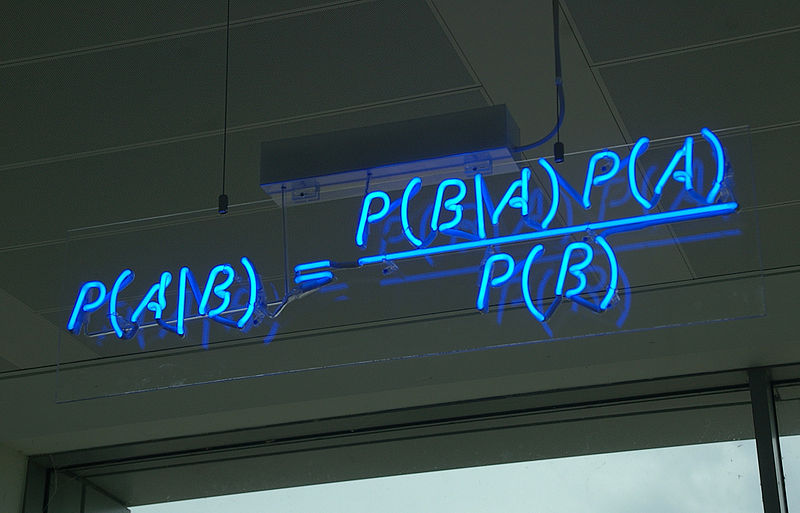
\includegraphics[width=11.11in]{images/bayes_neon}

\}

\textbackslash caption\{Bayes' theorem spelt out in blue neon. Source: \href{https://en.wikipedia.org/wiki/Bayes\%27_theorem}{Wikipedia}\}\label{fig:bayestheorem}
\textbackslash end\{figure\}

I don't know about you, but I need to think twice for not messing the letters around. I find it easier to remember Bayes' theorem written like this\footnote{When teaching Bayes' theorem, I am very much inspired by Tristan Mahr's slides from his introduction to Bayesian regression \url{https://www.tjmahr.com/bayes-intro-lecture-slides-2017/}}:

\[ \Pr(\text{hypothesis} \mid \text{data}) = \frac{ \Pr(\text{data} \mid \text{hypothesis}) \; \Pr(\text{hypothesis})}{\Pr(\text{data})} \]
\begin{rmdnote}
The \emph{hypothesis} is a working assumption about which you want to learn using \emph{data}. In capture--recapture analyses, the hypothesis might be a parameter like detection probability, or regression parameters in a relationship between survival probability and a covariate. Bayes' theorem tells us how to obtain the probability of a hypothesis given the data we have.
\end{rmdnote}

This is great because think about it, this is exactly what the scientific method is! We'd like to know how plausible some hypothesis is based on some data we collected, and possibly compare several hypotheses among them. In that respect, the Bayesian reasoning matches the scientific reasoning, which probably explains why the Bayesian framework is so natural for doing and understanding statistics.

You might ask then, why is Bayesian statistics not the default in statistics? Clearly, because of futile wars between male statisticians (including Ronald Fisher, Jerzy Neyman and Egon Sharpe Pearson among others), little progress was made for over two centuries. Also, until recently, there were practical problems to implement Bayes' theorem. Recent advances in computational power coupled with the development of new algorithms have led to a great increase in the application of Bayesian methods within the last three decades.

\hypertarget{what-is-the-bayesian-approach}{%
\section{What is the Bayesian approach?}\label{what-is-the-bayesian-approach}}

Typical statistical problems involve estimating a parameter (or several parameters) \(\theta\) with available data. To do so, you might be more used to the frequentist rather than the Bayesian method. The frequentist approach, and in particular maximum likelihood estimation (MLE), assumes that the parameters are fixed, and have unknown values to be estimated. Therefore classical estimates are generally point estimates of the parameters of interest. In contrast, the Bayesian approach assumes that the parameters are not fixed, and have some unknown distribution\footnote{A probability distribution is a mathematical expression that gives the probability for a random variable to take particular values. A probability distribution may be either discrete (e.g., the Bernoulli, Binomial or Poisson distribution) or continuous (e.g., the Gaussian distribution also known as the normal distribution)}.

The Bayesian approach is based upon the idea that you, as an experimenter, begin with some prior beliefs about the system. Then you collect data and update your prior beliefs on the basis of observations. These observations might arise from field work, lab work or from expertise of your esteemed colleagues. This updating process is based upon Bayes' theorem. Loosely, let's say \(A = \theta\) and \(B = \text{data}\), then Bayes' theorem gives you a way to estimate parameter \(\theta\) given the data you have:

\[{\color{red}{\Pr(\theta \mid \text{data})}} = \frac{\color{blue}{\Pr(\text{data} \mid \theta)} \times \color{green}{\Pr(\theta)}}{\color{orange}{\Pr(\text{data})}}.\]
Let's spend some time going through each quantity in this formula.

On the left-hand side is the \(\color{red}{\text{posterior distribution}}\). It represents what you know after having seen the data. This is the basis for inference and clearly what you're after, a distribution, possibly multivariate if you have more than one parameter.

On the right-hand side, there is the \(\color{blue}{\text{likelihood}}\). This quantity is the same as in the MLE approach. Yes, the Bayesian and frequentist approaches have the same likelihood at their core, which mostly explains why results often do not differ much. The likelihood captures the information you have in your data, given a model parameterized with \(\theta\).

Then we have the \(\color{green}{\text{prior distribution}}\). This quantity represents what you know before seeing the data. This is the source of much discussion about the Bayesian approach. It may be vague if you don't know anything about \(\theta\). Usually however, you never start from scratch, and you'd like your prior to reflect the information you have\footnote{Shall I include a section on sensitivity analyses in this chapter or later in the book? Cross-reference section in Survival chapter where prior elicitation is covered.}.

Last, we have \(\color{orange}{\Pr(\text{data})}\) which is sometimes called the average likelihood because it is obtained by integrating the likelihood with respect to the prior \(\color{orange}{\Pr(\text{data}) = \int{L(\text{data} \mid \theta)\Pr(\theta) d\theta}}\) so that the posterior is standardized, that is it integrates to one for the posterior to be a distribution. The average likelihood is an integral with dimension the number of parameters \(\theta\) you need to estimate. This quantity is difficult, if not impossible, to calculate in general. This is one of the reasons why the Bayesian method wasn't used until recently, and why we need algorithms to estimate posterior distributions as I illustrate in the next section.

\hypertarget{numerical-approx}{%
\section{Approximating posteriors via numerical integration}\label{numerical-approx}}

Let's take an example to illustrate Bayes' theorem. Say we capture, mark and release \(n = 57\) animals at the beginning of a winter, out of which we recapture \(y = 19\) animals alive\footnote{We used a similar example in \citet{king_bayesian_2009}}. We'd like to estimate winter survival \(\theta\).

\begin{Shaded}
\begin{Highlighting}[]
\NormalTok{y }\OtherTok{\textless{}{-}} \DecValTok{19} \CommentTok{\# nb of success}
\NormalTok{n }\OtherTok{\textless{}{-}} \DecValTok{57} \CommentTok{\# nb of attempts}
\end{Highlighting}
\end{Shaded}

We build our model first. Assuming all animals are independent of each other and have the same survival probability, then \(y\) the number of alive animals at the end of the winter is a binomial distribution\footnote{I follow \citet{mcelreathbook} and use labels on the right to help remember what each line is about.} with \(n\) trials and \(\theta\) the probability of success:

\begin{align*}
y &\sim \text{Binomial}(n, \theta) &\text{[likelihood]}
\end{align*}

This likelihood can be visualised in \texttt{R}:

\begin{Shaded}
\begin{Highlighting}[]
\NormalTok{grid }\OtherTok{\textless{}{-}} \FunctionTok{seq}\NormalTok{(}\DecValTok{0}\NormalTok{, }\DecValTok{1}\NormalTok{, }\FloatTok{0.01}\NormalTok{) }\CommentTok{\# grid of values for survival}
\NormalTok{likelihood }\OtherTok{\textless{}{-}} \FunctionTok{dbinom}\NormalTok{(y, n, grid) }\CommentTok{\# compute binomial likelihood}
\NormalTok{df }\OtherTok{\textless{}{-}} \FunctionTok{data.frame}\NormalTok{(}\AttributeTok{survival =}\NormalTok{ grid, }\AttributeTok{likelihood =}\NormalTok{ likelihood) }
\NormalTok{df }\SpecialCharTok{\%\textgreater{}\%}
  \FunctionTok{ggplot}\NormalTok{() }\SpecialCharTok{+} 
  \FunctionTok{aes}\NormalTok{(}\AttributeTok{x =}\NormalTok{ survival, }\AttributeTok{y =}\NormalTok{ likelihood) }\SpecialCharTok{+} 
  \FunctionTok{geom\_line}\NormalTok{(}\AttributeTok{size =} \FloatTok{1.5}\NormalTok{)}
\end{Highlighting}
\end{Shaded}

\begin{figure}
\centering
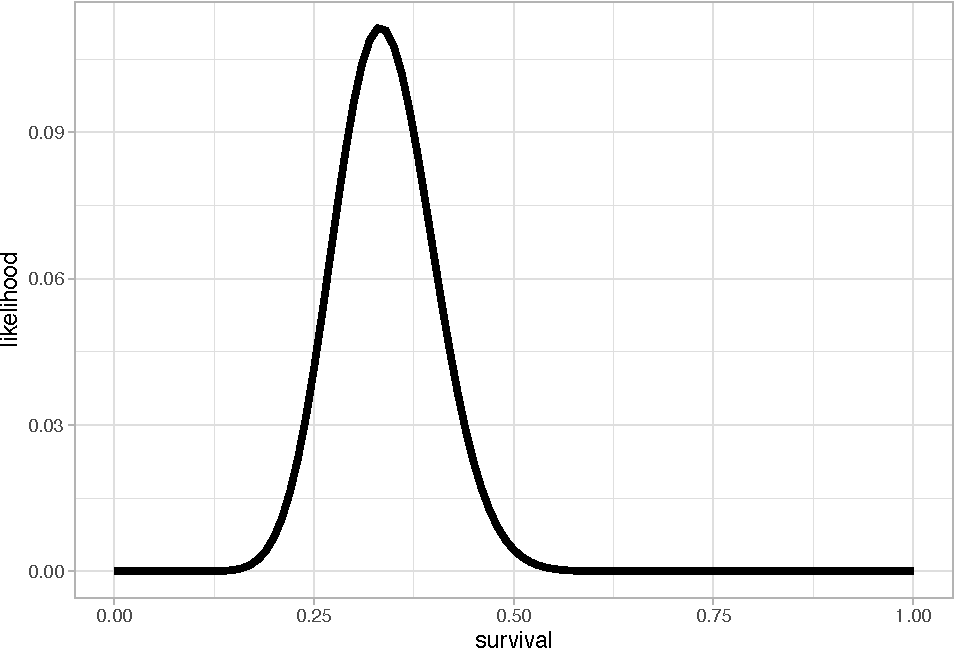
\includegraphics{banana-book_files/figure-latex/binlik-1.pdf}
\caption{\label{fig:binlik}Binomial likelihood with \(n = 57\) released animals and \(y = 19\) survivors after winter. The value of survival (on the x-axis) that corresponds to the maximum of the likelihood function (on the y-axis) is the MLE, or the proportion of success in this example, close to 0.33.}
\end{figure}

Besides the likelihood, priors are another component of the model in the Bayesian approach. For a parameter that is a probability, the one thing we know is that the prior should be a continuous random variable that lies between 0 and 1. To reflect that, we often go for the uniform distribution \(U(0,1)\) to imply \emph{vague} priors. Here vague means that survival has, before we see the data, the same probability of falling between 0.1 and 0.2 and between 0.8 and 0.9, for example.

\begin{align*}
\theta &\sim \text{Uniform}(0, 1) &\text{[prior for }\theta \text{]}
\end{align*}

Now we apply Bayes' theorem. We write a \texttt{R} function that computes the product of the likelihood times the prior, or the numerator in Bayes' theorem: \(\Pr(\text{data} \mid \theta) \times \Pr(\theta)\)

\begin{Shaded}
\begin{Highlighting}[]
\NormalTok{numerator }\OtherTok{\textless{}{-}} \ControlFlowTok{function}\NormalTok{(theta) }\FunctionTok{dbinom}\NormalTok{(y, n, theta) }\SpecialCharTok{*} \FunctionTok{dunif}\NormalTok{(theta, }\DecValTok{0}\NormalTok{, }\DecValTok{1}\NormalTok{)}
\end{Highlighting}
\end{Shaded}

We write another function that calculates the denominator, the average likelihood: \(\Pr(\text{data}) = \int{L(\theta \mid \text{data}) \Pr(\theta) d\theta}\)

\begin{Shaded}
\begin{Highlighting}[]
\NormalTok{denominator }\OtherTok{\textless{}{-}} \FunctionTok{integrate}\NormalTok{(numerator,}\DecValTok{0}\NormalTok{,}\DecValTok{1}\NormalTok{)}\SpecialCharTok{$}\NormalTok{value}
\end{Highlighting}
\end{Shaded}

We use the \texttt{R} function \texttt{integrate} to calculate the integral in the denominator, which implements quadrature techniques to divide in little squares the area underneath the curve delimited by the function to integrate (here the numerator), and count them.

Then we get a numerical approximation of the posterior in Figure \ref{fig:numapprox} by applying Bayes' theorem.

\begin{Shaded}
\begin{Highlighting}[]
\NormalTok{grid }\OtherTok{\textless{}{-}} \FunctionTok{seq}\NormalTok{(}\DecValTok{0}\NormalTok{, }\DecValTok{1}\NormalTok{, }\FloatTok{0.01}\NormalTok{) }\CommentTok{\# grid of values for theta}
\NormalTok{numerical\_posterior }\OtherTok{\textless{}{-}} \FunctionTok{data.frame}\NormalTok{(}\AttributeTok{survival =}\NormalTok{ grid, }
                                  \AttributeTok{posterior =} \FunctionTok{numerator}\NormalTok{(grid)}\SpecialCharTok{/}\NormalTok{denominator) }\CommentTok{\# Bayes\textquotesingle{} theorem}
\NormalTok{numerical\_posterior }\SpecialCharTok{\%\textgreater{}\%}
  \FunctionTok{ggplot}\NormalTok{() }\SpecialCharTok{+}
  \FunctionTok{aes}\NormalTok{(}\AttributeTok{x =}\NormalTok{ survival, }\AttributeTok{y =}\NormalTok{ posterior) }\SpecialCharTok{+} 
  \FunctionTok{geom\_line}\NormalTok{(}\AttributeTok{size =} \FloatTok{1.5}\NormalTok{)}
\end{Highlighting}
\end{Shaded}

\begin{figure}
\centering
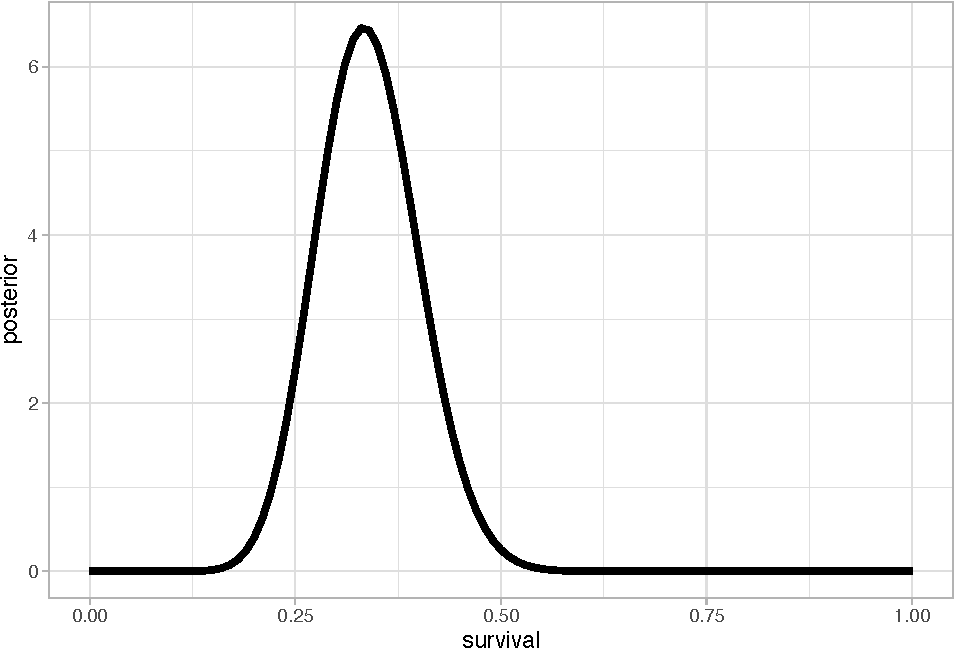
\includegraphics{banana-book_files/figure-latex/numapprox-1.pdf}
\caption{\label{fig:numapprox}Winter survival posterior distribution obtained by numerical integration.}
\end{figure}

How good is our numerical approximation of survival posterior distribution? Ideally, we would want to compare the approximation to the true posterior distribution. Although a closed-form expression for the posterior distribution is in general intractable, when you combine a binomial likelihood together with a beta distribution as a prior, then the posterior distribution is also a beta distribution, which makes it amenable to all sorts of exact calculations\footnote{We say that the beta distribution is the conjugate prior distribution for the binomial distribution.}. The beta distribution is continuous between 0 and 1, and extends the uniform distribution to situations where not all outcomes are equally likely. It has two parameters \(a\) and \(b\) that control its shape (Figure \ref{fig:betadistribution}).



\begin{figure}
\centering
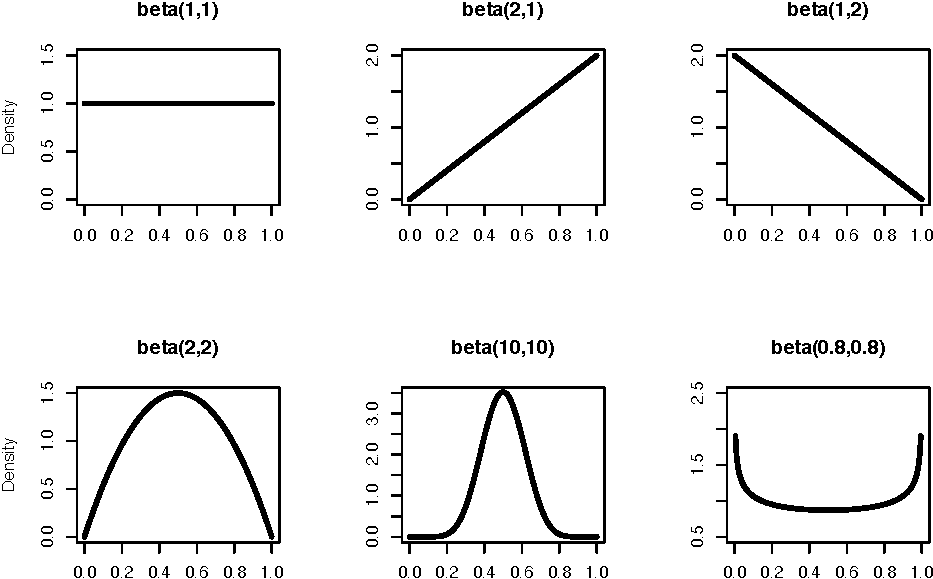
\includegraphics{banana-book_files/figure-latex/betadistribution-1.pdf}
\caption{\label{fig:betadistribution}The distribution beta(\(a\),\(b\)) for different values of \(a\) and \(b\). Note that for \(a = b = 1\), we get the uniform distribution between 0 and 1 in the top left panel. When \(a\) and \(b\) are equal, the distribution is symmetric, and the bigger \(a\) and \(b\), the more peaked the distribution or the smaller the variance.}
\end{figure}

If the likelihood of the data \(y\) is binomial with \(n\) trials and probability of success \(\theta\), and the prior is a beta distribution with parameters \(a\) and \(b\), then the posterior is a beta distribution with parameters \(a + y\) and \(b + n - y\)\footnote{\textbf{provide a sketch of the proof}}. In our example, we have \(n = 57\) trials and \(y = 19\) animals that survived and a uniform prior between 0 and 1 or a beta distribution with parameters \(a = b = 1\), therefore survival has a beta posterior distribution with parameters 20 and 39. In Figure \ref{fig:compar}, we superimpose the exact posterior and the numerical approximation. Clearly, the two distributions are indistinguishable, suggesting that the numerical approximation is more than fine.
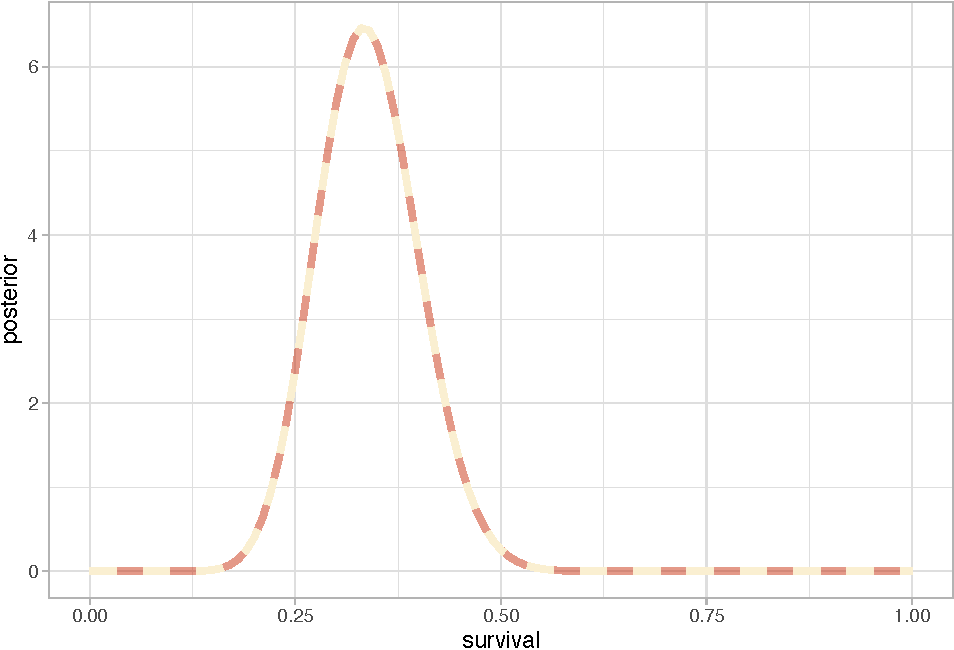
\includegraphics{banana-book_files/figure-latex/compar-1.pdf}

In our example, we have a single parameter to estimate, winter survival. This means dealing with a one-dimensional integral in the denominator which is pretty easy with quadrature techniques and the \texttt{R} function \texttt{integrate()}. Now what if we had multiple parameters? For example, imagine you'd like to fit a capture-recapture model with detection probability \(p\) and regression parameters \(\alpha\) and \(\beta\) for the intercept and slope of a relationship between survival probability and a covariate, then Bayes' theorem gives you the posterior distribution of all three parameters together:

\[ \Pr(\alpha, \beta, p \mid \text{data}) = \frac{ \Pr(\text{data} \mid \alpha, \beta, p) \times \Pr(\alpha, \beta, p)}{\iiint \, \Pr(\text{data} \mid \alpha, \beta, p) \Pr(\alpha, \beta, p) d\alpha d\beta dp} \]
There are two computational challenges with this formula. First, do we really wish to calculate a three-dimensional integral? The answer is no, one-dimensional and two-dimensional integrals are so much further we can go with standard methods. Second, we're more interested in a posterior distribution for each parameter separately than the joint posterior distribution. The so-called marginal distribution of \(p\) for example is obtained by integrating over all the other parameters -- a two-dimensional integral in this example. Now imagine with tens or hundreds of parameters to estimate, these integrals become highly multi-dimensional and simply intractable. In the next section, I introduce powerful simulation methods to circumvent this issue.

\hypertarget{markov-chain-monte-carlo-mcmc}{%
\section{Markov chain Monte Carlo (MCMC)}\label{markov-chain-monte-carlo-mcmc}}

In the early 1990s, statisticians rediscovered work from the 1950's in physics. In a famous paper that would lay the fundations of modern Bayesian statistics (Figure \ref{fig:mcmcpaper}), the authors use simulations to approximate posterior distributions with some precision by drawing large samples. This is a neat trick to avoid explicit calculation of the multi-dimensional integrals we struggle with when using Bayes' theorem.

\begin{figure}

{\centering 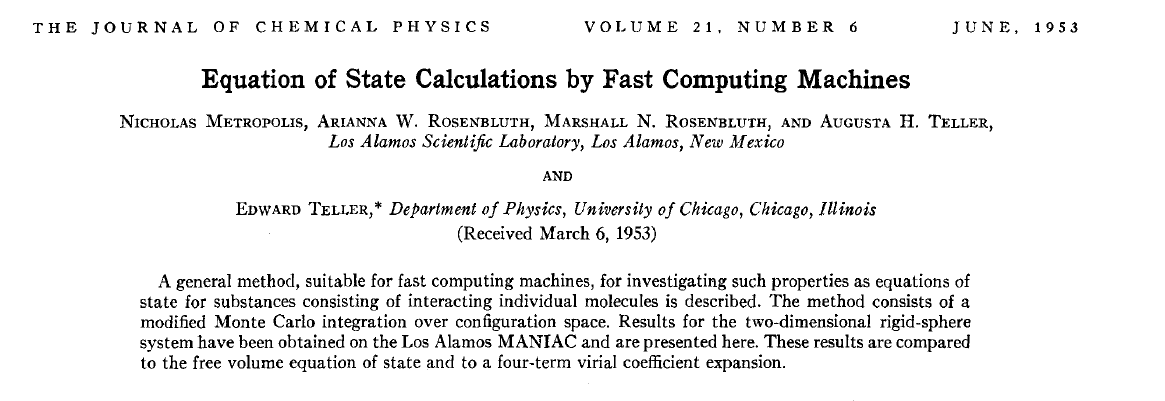
\includegraphics[width=16.18in]{images/metropolis} 

}

\caption{MCMC article cover. Source: [The Journal of Chemical Physics](https://aip.scitation.org/doi/10.1063/1.1699114)}\label{fig:mcmcpaper}
\end{figure}

These simulation algorithms are called Markov chain Monte Carlo (MCMC), and they definitely gave a boost to Bayesian statistics. There are two parts in MCMC, Markov chain and Monte Carlo, let's try and make sense of these terms.

\hypertarget{monte-carlo-integration}{%
\subsection{Monte Carlo integration}\label{monte-carlo-integration}}

What does Monte Carlo stand for? Monte Carlo integration is a simulation technique to calculate integrals of any function \(f\) of random variable \(X\) with distribution \(\Pr(X)\) say \(\int f(X) \Pr(X)dX\). You draw values \(X_1,\ldots,X_k\) from \(\Pr(X)\) the distribution of \(X\), apply function \(f\) to these values, then calculate the mean of these new values \(\displaystyle{\frac{1}{k}}\sum_{i=1}^k{f(X_i)}\) to approximate the integral. How is Monte Carlo integration used in a Bayesian context? The posterior distribution contains all the information we need about the parameter to be estimated. When dealing with many parameters however, you may want to summarise posterior results by calculating numerical summaries. The simplest numerical summary is the mean of the posterior distribution, \(E(\theta) = \int \theta \Pr(\theta|\text{data})\), where \(X\) is \(\theta\) now and \(f\) is the identity function. Posterior mean can be calculated with Monte Carlo integration:

\begin{Shaded}
\begin{Highlighting}[]
\NormalTok{sample\_from\_posterior }\OtherTok{\textless{}{-}} \FunctionTok{rbeta}\NormalTok{(}\DecValTok{1000}\NormalTok{, }\DecValTok{20}\NormalTok{, }\DecValTok{39}\NormalTok{) }\CommentTok{\# draw 1000 values from posterior survival beta(20,39)}
\FunctionTok{mean}\NormalTok{(sample\_from\_posterior) }\CommentTok{\# compute mean with Monte Carlo integration}
\DocumentationTok{\#\# [1] 0.3429}
\end{Highlighting}
\end{Shaded}

You may check that the mean we have just calculated matches closely the expectation of a beta distribution\footnote{If \(X\) is a random variable with distribution \(\text{beta}(a, b)\), then \(E(X) = \displaystyle{\frac{a}{a + b}}\)}:

\begin{Shaded}
\begin{Highlighting}[]
\DecValTok{20}\SpecialCharTok{/}\NormalTok{(}\DecValTok{20}\SpecialCharTok{+}\DecValTok{39}\NormalTok{) }\CommentTok{\# expectation of beta(20,39)}
\DocumentationTok{\#\# [1] 0.339}
\end{Highlighting}
\end{Shaded}

Another useful numerical summary is the credible interval within which our parameter falls with some probability, usually 0.95 hence a 95\(\%\) credible interval. Finding the bounds of a credible interval requires calculating quantiles, which in turn involves integrals and the use of Monte Carlo integration. A 95\(\%\) credible interval for winter survival can be obtained in \texttt{R} with:

\begin{Shaded}
\begin{Highlighting}[]
\FunctionTok{quantile}\NormalTok{(sample\_from\_posterior, }\AttributeTok{probs =} \FunctionTok{c}\NormalTok{(}\FloatTok{2.5}\SpecialCharTok{/}\DecValTok{100}\NormalTok{, }\FloatTok{97.5}\SpecialCharTok{/}\DecValTok{100}\NormalTok{))}
\DocumentationTok{\#\#   2.5\%  97.5\% }
\DocumentationTok{\#\# 0.2280 0.4628}
\end{Highlighting}
\end{Shaded}

\hypertarget{markov-chains}{%
\subsection{Markov chains}\label{markov-chains}}

What is a Markov chain? A Markov chain is a random sequence of numbers, in which each number depends only on the previous number. An example is the weather in my home town in Southern France, Montpellier, in which a sunny day is most likely to be followed by another sunny day, say with probability 0.8, and a rainy day is rarely followed by another rainy day, say with probability 0.1. The dynamic of this Markov chain is captured by the transition matrix \(\mathbf{\Gamma}\):
\[
\begin{matrix}
& \\
\mathbf{\Gamma} = 
    \left ( \vphantom{ \begin{matrix} 12 \\ 12 \end{matrix} } \right .
\end{matrix}
\hspace{-1.2em}
\begin{matrix}
    \text{sunny tomorrow} & \text{rainy tomorrow} \\ 
0.8 & 0.2 \\ 
0.9 & 0.1 \\ 
\end{matrix}
\hspace{-0.2em}
\begin{matrix}
& \\
\left . \vphantom{ \begin{matrix} 12 \\ 12 \\ 12 \end{matrix} } \right )
    \begin{matrix}
    \text{sunny today} \\ \text{rainy today}
    \end{matrix}
\end{matrix}
\]
In rows the weather today, and in columns the weather tomorrow. The cells give the probability of a sunny or rainy day tomorrow, given the day is sunny or rainy today. Under certain conditions\footnote{The Markov chain is irreducible and aperiodic.}, a Markov chain will converge to a unique stationary distribution. In our weather example, let's run the Markov chain for 20 steps:

\begin{Shaded}
\begin{Highlighting}[]
\NormalTok{weather }\OtherTok{\textless{}{-}} \FunctionTok{matrix}\NormalTok{(}\FunctionTok{c}\NormalTok{(}\FloatTok{0.8}\NormalTok{, }\FloatTok{0.2}\NormalTok{, }\FloatTok{0.9}\NormalTok{, }\FloatTok{0.1}\NormalTok{), }\AttributeTok{nrow =} \DecValTok{2}\NormalTok{, }\AttributeTok{byrow =}\NormalTok{ T) }\CommentTok{\# transition matrix}
\NormalTok{steps }\OtherTok{\textless{}{-}} \DecValTok{20}
\ControlFlowTok{for}\NormalTok{ (i }\ControlFlowTok{in} \DecValTok{1}\SpecialCharTok{:}\NormalTok{steps)\{}
\NormalTok{  weather }\OtherTok{\textless{}{-}}\NormalTok{ weather }\SpecialCharTok{\%*\%}\NormalTok{ weather }\CommentTok{\# matrix multiplication}
\NormalTok{\}}
\FunctionTok{round}\NormalTok{(weather, }\DecValTok{2}\NormalTok{) }\CommentTok{\# matrix product after 20 steps}
\DocumentationTok{\#\#      [,1] [,2]}
\DocumentationTok{\#\# [1,] 0.82 0.18}
\DocumentationTok{\#\# [2,] 0.82 0.18}
\end{Highlighting}
\end{Shaded}

Each row of the transition matrix converges to the same distribution \((0.82, 0.18)\) as the number of steps increases. Convergence happens no matter which state you start in, and you always have probability 0.82 of the day being sunny and 0.18 of the day being rainy.

Back to MCMC, the core idea is that you can build a Markov chain with a given stationary distribution set to be the desired posterior distribution.

\begin{rmdnote}
Putting Monte Carlo and Markov chains together, MCMC allows us to generate a sample of values (Markov chain) whose distribution converges to the posterior distribution, and we can use this sample of values to calculate any posterior summaries (Monte Carlo), such as posterior means and credible intervals.
\end{rmdnote}

\hypertarget{metropolis-algorithm}{%
\subsection{Metropolis algorithm}\label{metropolis-algorithm}}

There are several ways of constructing Markov chains for Bayesian inference\footnote{You might have heard about the Metropolis-Hastings or the Gibbs sampler. Have a look to \url{https://github.com/chi-feng/mcmc-demo} for an interactive gallery of MCMC algorithms.}. Here I illustrate the Metropolis algorithm and how to implement it in practice\footnote{This presentation is largely inspired by \citet{alberthu2019}}.

Let's go back to our example on animal survival estimation. We illustrate sampling from survival posterior distribution. We write functions for likelihood, prior and posterior.

\begin{Shaded}
\begin{Highlighting}[]
\CommentTok{\# 19 animals recaptured alive out of 57 captured, marked and released}
\NormalTok{survived }\OtherTok{\textless{}{-}} \DecValTok{19}
\NormalTok{released }\OtherTok{\textless{}{-}} \DecValTok{57}

\CommentTok{\# binomial log{-}likelihood function}
\NormalTok{loglikelihood }\OtherTok{\textless{}{-}} \ControlFlowTok{function}\NormalTok{(x, p)\{}
  \FunctionTok{dbinom}\NormalTok{(}\AttributeTok{x =}\NormalTok{ x, }\AttributeTok{size =}\NormalTok{ released, }\AttributeTok{prob =}\NormalTok{ p, }\AttributeTok{log =} \ConstantTok{TRUE}\NormalTok{)}
\NormalTok{\}}

\CommentTok{\# uniform prior density}
\NormalTok{logprior }\OtherTok{\textless{}{-}} \ControlFlowTok{function}\NormalTok{(p)\{}
  \FunctionTok{dunif}\NormalTok{(}\AttributeTok{x =}\NormalTok{ p, }\AttributeTok{min =} \DecValTok{0}\NormalTok{, }\AttributeTok{max =} \DecValTok{1}\NormalTok{, }\AttributeTok{log =} \ConstantTok{TRUE}\NormalTok{)}
\NormalTok{\}}

\CommentTok{\# posterior density function (log scale)}
\NormalTok{posterior }\OtherTok{\textless{}{-}} \ControlFlowTok{function}\NormalTok{(x, p)\{}
  \FunctionTok{loglikelihood}\NormalTok{(x, p) }\SpecialCharTok{+} \FunctionTok{logprior}\NormalTok{(p) }\CommentTok{\# {-} log(Pr(data))}
\NormalTok{\}}
\end{Highlighting}
\end{Shaded}

The Metropolis algorithm works as follows:

\begin{enumerate}
\def\labelenumi{\arabic{enumi}.}
\item
  We pick a value of the parameter to be estimated. This is where we start our Markov chain -- this is a \emph{starting} value.
\item
  To decide where to go next, we propose to move away from the current value of the parameter -- this is a \emph{candidate} value. To do so, we add to the current value some random value from e.g.~a normal distribution with some variance -- this is a \emph{proposal} distribution. The Metropolis algorithm is a particular case of the Metropolis-Hastings algorithm with symmetric proposals.
\item
  We compute the ratio of the probabilities at the candidate and current locations \(R=\displaystyle{\frac{{\Pr(\text{candidate}|\text{data})}}{{\Pr(\text{current}|\text{data})}}}\). This is where the magic of MCMC happens, in that \(\Pr(\text{data})\), the denominator in the Bayes' theorem, appears in both the numerator and the denominator in \(R\) therefore cancels out and does not need to be calculated.
\end{enumerate}

\begin{enumerate}
\def\labelenumi{\arabic{enumi}.}
\setcounter{enumi}{3}
\item
  If the posterior at the candidate location \(\Pr(\text{candidate}|\text{data})\) is higher than at the current location \(\Pr(\text{current}|\text{data})\), in other words when the candidate value is more plausible than the current value, we definitely accept the candidate value. If not, then we accept the candidate value with probability \(R\) and reject with probability \(1-R\). For example, if the candidate value is ten times less plausible than the current value, then we accept with probability 0.1 and reject with probability 0.9. How does it work in practice? We use a continuous spinner that lands somewhere between 0 and 1 -- call the random spin \(X\). If \(X\) is smaller than \(R\), we move to the candidate location, otherwise we remain at the current location. We do not want to accept or reject too often. In practice, the Metropolis algorithm should have an acceptance probability between 0.2 and 0.4, which can be achieved by \emph{tuning} the variance of the normal proposal distribution.
\item
  We repeat 2-4 a number of times -- or \emph{steps}.
\end{enumerate}

Enough of the theory, let's implement the Metropolis algorithm in \texttt{R}. Let's start by setting the scene.

\begin{Shaded}
\begin{Highlighting}[]
\NormalTok{steps }\OtherTok{\textless{}{-}} \DecValTok{100} \CommentTok{\# number of steps}
\NormalTok{theta.post }\OtherTok{\textless{}{-}} \FunctionTok{rep}\NormalTok{(}\ConstantTok{NA}\NormalTok{, steps) }\CommentTok{\# vector to store samples}
\NormalTok{accept }\OtherTok{\textless{}{-}} \FunctionTok{rep}\NormalTok{(}\ConstantTok{NA}\NormalTok{, steps) }\CommentTok{\# keep track of accept/reject}
\FunctionTok{set.seed}\NormalTok{(}\DecValTok{1234}\NormalTok{) }\CommentTok{\# for reproducibility}
\end{Highlighting}
\end{Shaded}

Now follow the 5 steps we've just described. First, we pick a starting value, and store it (step 1).

\begin{Shaded}
\begin{Highlighting}[]
\NormalTok{inits }\OtherTok{\textless{}{-}} \FloatTok{0.5}
\NormalTok{theta.post[}\DecValTok{1}\NormalTok{] }\OtherTok{\textless{}{-}}\NormalTok{ inits}
\NormalTok{accept[}\DecValTok{1}\NormalTok{] }\OtherTok{\textless{}{-}} \DecValTok{1}
\end{Highlighting}
\end{Shaded}

Then, we need a function to propose a candidate value. We add a value taken from a normal distribution with mean zero and standard deviation we call \emph{away}. We work on the logit scale to make sure the candidate value for survival lies between 0 and 1.

\begin{Shaded}
\begin{Highlighting}[]
\NormalTok{move }\OtherTok{\textless{}{-}} \ControlFlowTok{function}\NormalTok{(x, }\AttributeTok{away =} \DecValTok{1}\NormalTok{)\{ }\CommentTok{\# by default, standard deviation of the proposal distribution is 1}
\NormalTok{  logitx }\OtherTok{\textless{}{-}} \FunctionTok{log}\NormalTok{(x }\SpecialCharTok{/}\NormalTok{ (}\DecValTok{1} \SpecialCharTok{{-}}\NormalTok{ x)) }\CommentTok{\# apply logit transform ({-}infinity,+infinity)}
\NormalTok{  logit\_candidate }\OtherTok{\textless{}{-}}\NormalTok{ logitx }\SpecialCharTok{+} \FunctionTok{rnorm}\NormalTok{(}\DecValTok{1}\NormalTok{, }\DecValTok{0}\NormalTok{, away) }\CommentTok{\# add a value taken from N(0,sd=away) to current value}
\NormalTok{  candidate }\OtherTok{\textless{}{-}} \FunctionTok{plogis}\NormalTok{(logit\_candidate) }\CommentTok{\# back{-}transform (0,1)}
  \FunctionTok{return}\NormalTok{(candidate)}
\NormalTok{\}}
\end{Highlighting}
\end{Shaded}

Now we're ready for steps 2, 3 and 4. We write a loop to take care of step 5. We start at initial value 0.5 and run the algorithm for 100 steps or iterations.

\begin{Shaded}
\begin{Highlighting}[]
\ControlFlowTok{for}\NormalTok{ (t }\ControlFlowTok{in} \DecValTok{2}\SpecialCharTok{:}\NormalTok{steps)\{ }\CommentTok{\# repeat steps 2{-}4 (step 5)}
  
  \CommentTok{\# propose candidate value for survival (step 2)}
\NormalTok{  theta\_star }\OtherTok{\textless{}{-}} \FunctionTok{move}\NormalTok{(theta.post[t}\DecValTok{{-}1}\NormalTok{])}
  
  \CommentTok{\# calculate ratio R (step 3)}
\NormalTok{  pstar }\OtherTok{\textless{}{-}} \FunctionTok{posterior}\NormalTok{(survived, }\AttributeTok{p =}\NormalTok{ theta\_star)  }
\NormalTok{  pprev }\OtherTok{\textless{}{-}} \FunctionTok{posterior}\NormalTok{(survived, }\AttributeTok{p =}\NormalTok{ theta.post[t}\DecValTok{{-}1}\NormalTok{])}
\NormalTok{  logR }\OtherTok{\textless{}{-}}\NormalTok{ pstar }\SpecialCharTok{{-}}\NormalTok{ pprev }\CommentTok{\# likelihood and prior are on the log scale}
\NormalTok{  R }\OtherTok{\textless{}{-}} \FunctionTok{exp}\NormalTok{(logR)}
  
  \CommentTok{\# accept candidate value or keep current value (step 4)}
\NormalTok{  X }\OtherTok{\textless{}{-}} \FunctionTok{runif}\NormalTok{(}\DecValTok{1}\NormalTok{, }\DecValTok{0}\NormalTok{, }\DecValTok{1}\NormalTok{) }\CommentTok{\# spin continuous spinner}
  \ControlFlowTok{if}\NormalTok{ (X }\SpecialCharTok{\textless{}}\NormalTok{ R)\{}
\NormalTok{    theta.post[t] }\OtherTok{\textless{}{-}}\NormalTok{ theta\_star }\CommentTok{\# accept candidate value}
\NormalTok{    accept[t] }\OtherTok{\textless{}{-}} \DecValTok{1} \CommentTok{\# accept}
\NormalTok{  \}}
  \ControlFlowTok{else}\NormalTok{\{}
\NormalTok{    theta.post[t] }\OtherTok{\textless{}{-}}\NormalTok{ theta.post[t}\DecValTok{{-}1}\NormalTok{] }\CommentTok{\# keep current value}
\NormalTok{    accept[t] }\OtherTok{\textless{}{-}} \DecValTok{0} \CommentTok{\# reject}
\NormalTok{  \}}
\NormalTok{\}}
\end{Highlighting}
\end{Shaded}

We get the following values.

\begin{Shaded}
\begin{Highlighting}[]
\FunctionTok{head}\NormalTok{(theta.post) }\CommentTok{\# first values}
\DocumentationTok{\#\# [1] 0.5000 0.2302 0.2906 0.2906 0.2980 0.2980}
\FunctionTok{tail}\NormalTok{(theta.post) }\CommentTok{\# last values}
\DocumentationTok{\#\# [1] 0.2622 0.2622 0.2622 0.3727 0.3232 0.3862}
\end{Highlighting}
\end{Shaded}

Visually, you may look at the chain in Figure \ref{fig:chain} called a trace plot.

\begin{figure}

{\centering 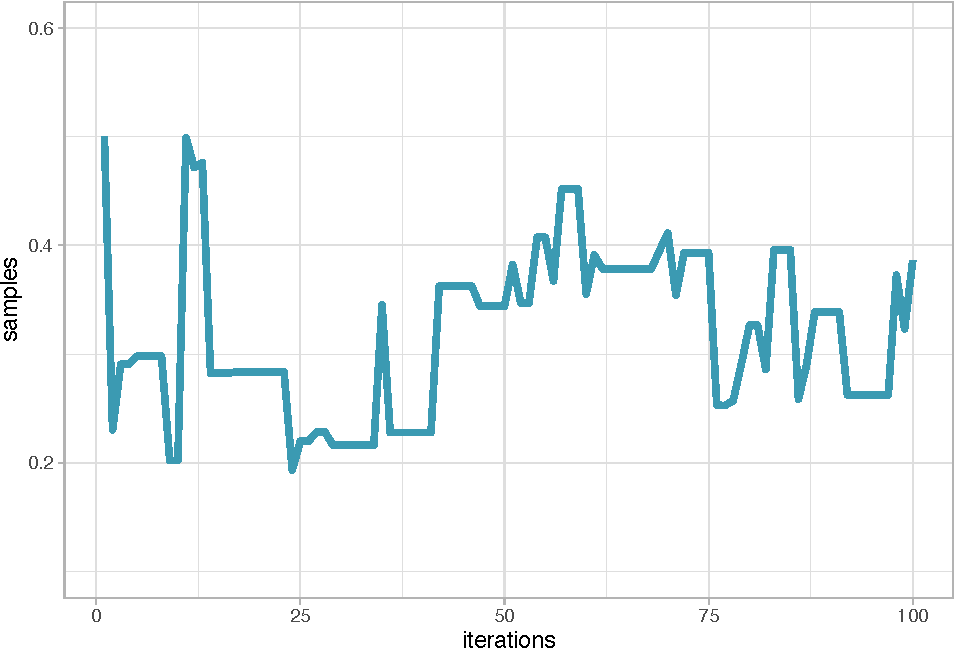
\includegraphics{banana-book_files/figure-latex/chain-1} 

}

\caption{Visualisation of a Markov chain starting at value 0.5, with steps or iterations on the x-axis, and samples on the y-axis. This graphical representation is called a trace plot.}\label{fig:chain}
\end{figure}

The acceptance probability is the average number of times we accepted a candidated value, which is 0.44 and almost satisfying.

Can we run another chain and start at initial value 0.2 this time? Yes, just go through the same algorithm again, and visualise the results in Figure \ref{fig:twochains}.

\begin{figure}

{\centering 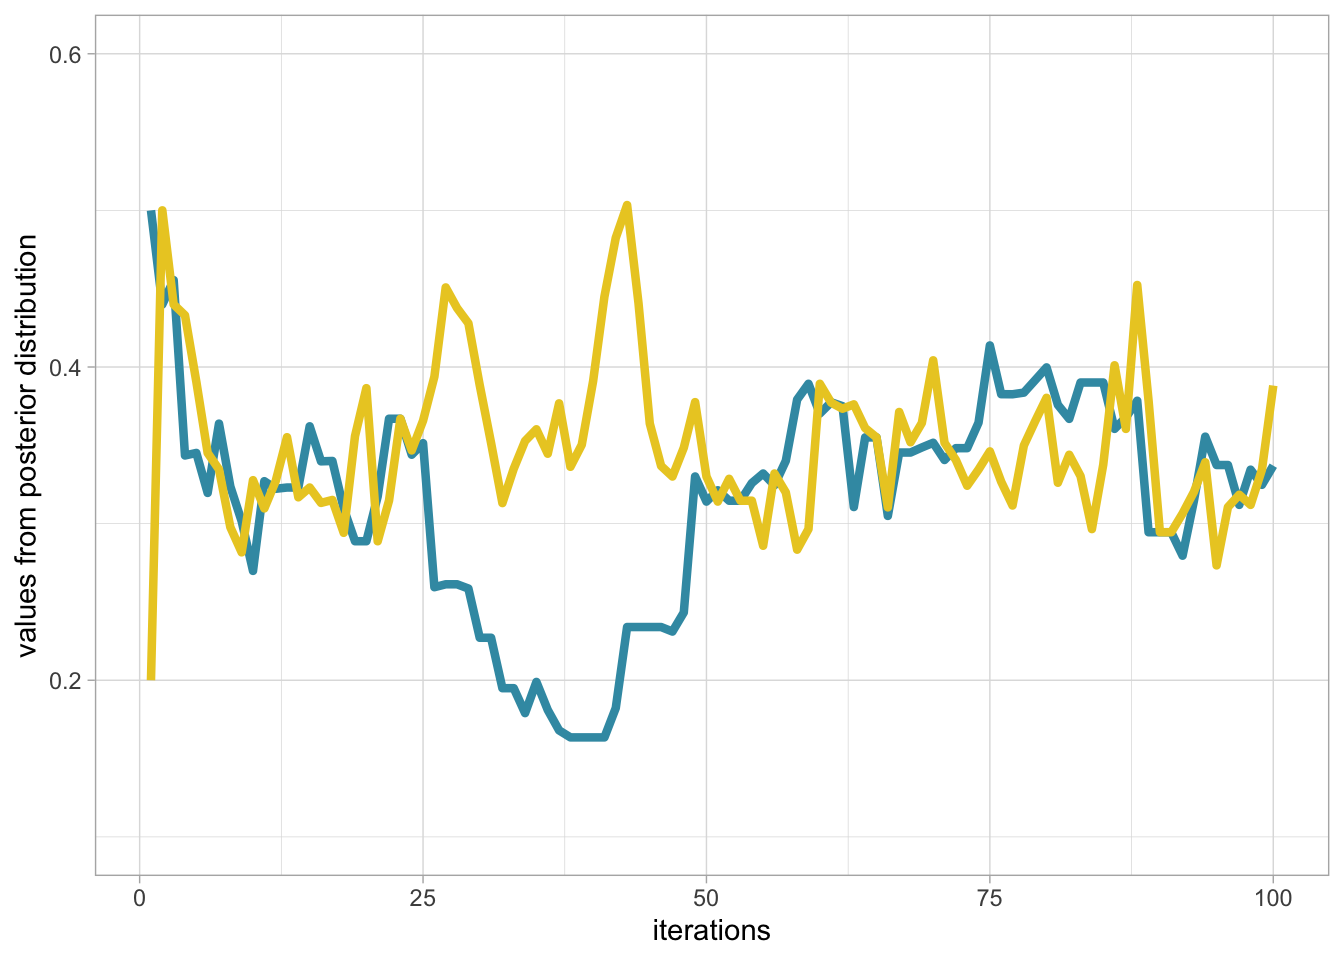
\includegraphics{banana-book_files/figure-latex/twochains-1} 

}

\caption{Trace plot of survival for two chains starting at 0.2 (yellow) and 0.5 (blue) run for 100 steps.}\label{fig:twochains}
\end{figure}

Notice that we do not get the exact same results because the algorithm is stochastic. The question is to know whether we have reached the stationary distribution. Let's increase the number of steps and run a chain with 5000 iterations as in Figure \ref{fig:longchain}.

\begin{figure}

{\centering 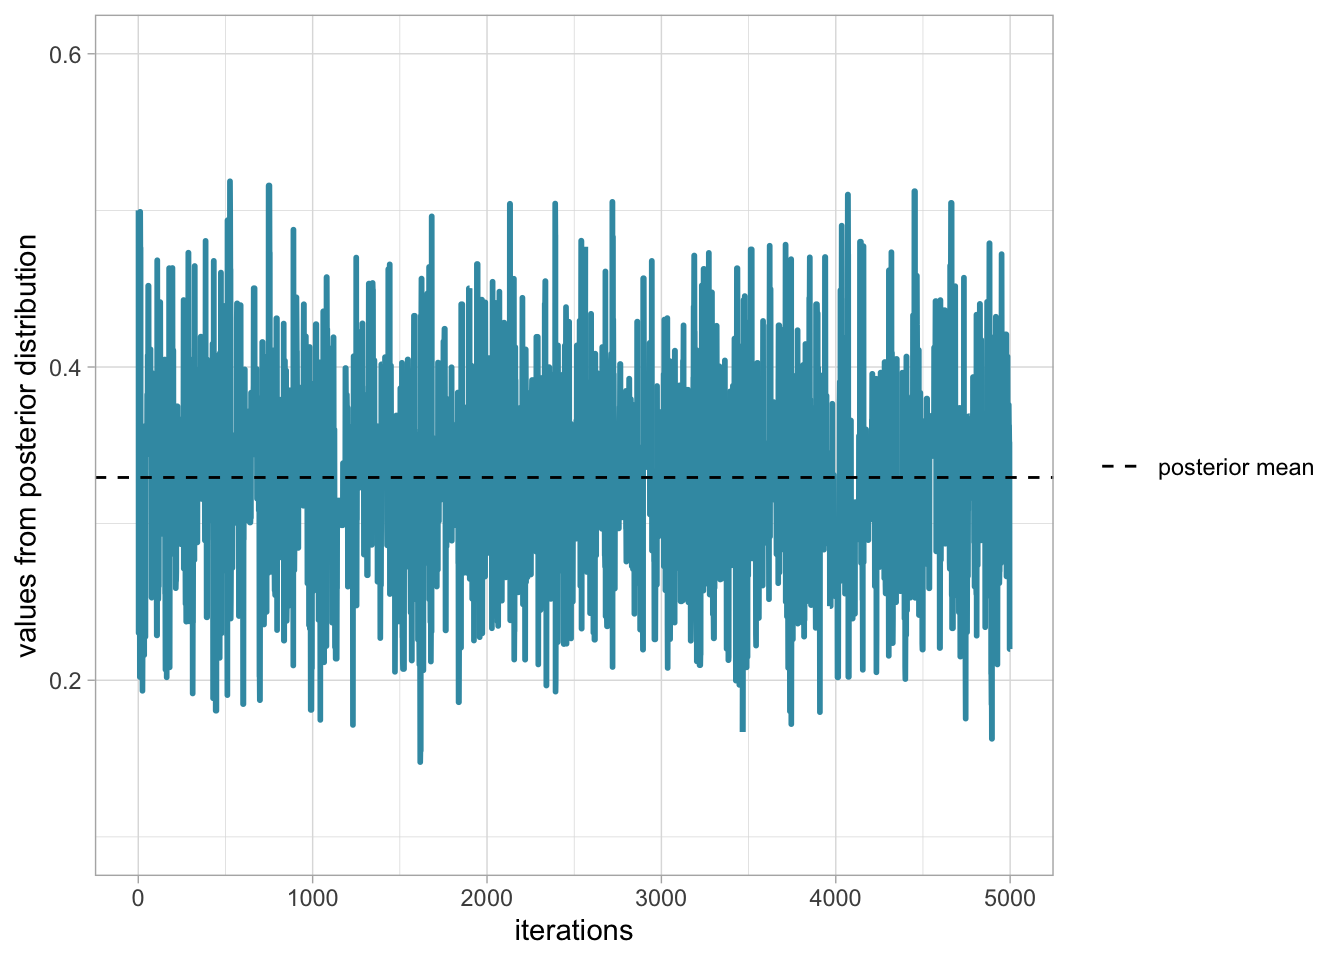
\includegraphics{banana-book_files/figure-latex/longchain-1} 

}

\caption{Trace plot of survival for a chain starting at 0.5 and 1000 steps.}\label{fig:longchain}
\end{figure}

This is what we're after, a trace plot that looks like a beautiful lawn, see Section \ref{convergence-diag}. I find it informative to look at the animated version of Figure \ref{fig:longchain}, it helps understanding the stochastic behavior of the algorithm, and also to realise how the chains converge to their stationary distribution, see Figure \ref{fig:animlongchain}.

\begin{figure}

{\centering \includegraphics[width=1\linewidth]{images/traceplotMCMC} 

}

\caption{Animated trace plot of survival with three chains starting at 0.2, 0.5 and 0.7 run for 1000 steps.}\label{fig:animlongchain}
\end{figure}

Once the stationary distribution is reached, you may regard the realisations of the Markov chain as a sample from the posterior distribution, and obtain numerical summaries. In the next section, we consider several important implementation issues.

\hypertarget{convergence-diag}{%
\section{Assessing convergence}\label{convergence-diag}}

\begin{rmdnote}
When implementing MCMC, we need to determine how long it takes for our Markov chain to converge to the target distribution, and the number of iterations we need after achieving convergence to get reasonable Monte Carlo estimates of numerical summaries (posterior means and credible intervals).
\end{rmdnote}

\hypertarget{burn-in}{%
\subsection{Burn-in}\label{burn-in}}

In practice, we discard observations from the start of the Markov chain and just use observations from the chain once it has converged. The initial observations that we discard are usually referred to as the \emph{burn-in}.

The simplest method to determine the length of the burn-in period is to look at trace plots. Going back to our example, we see from the trace plot in Figure \ref{fig:burnin} that we need at least 100 iterations to achieve convergence toward an average survival around 0.3. It is always better to be conservative when specifying the length of the burn-in period, and in this example, we would use 250 or even 500 iterations as a burn-in. The length of the burn-in period can be determined by performing preliminary MCMC short runs.

\begin{figure}
\centering
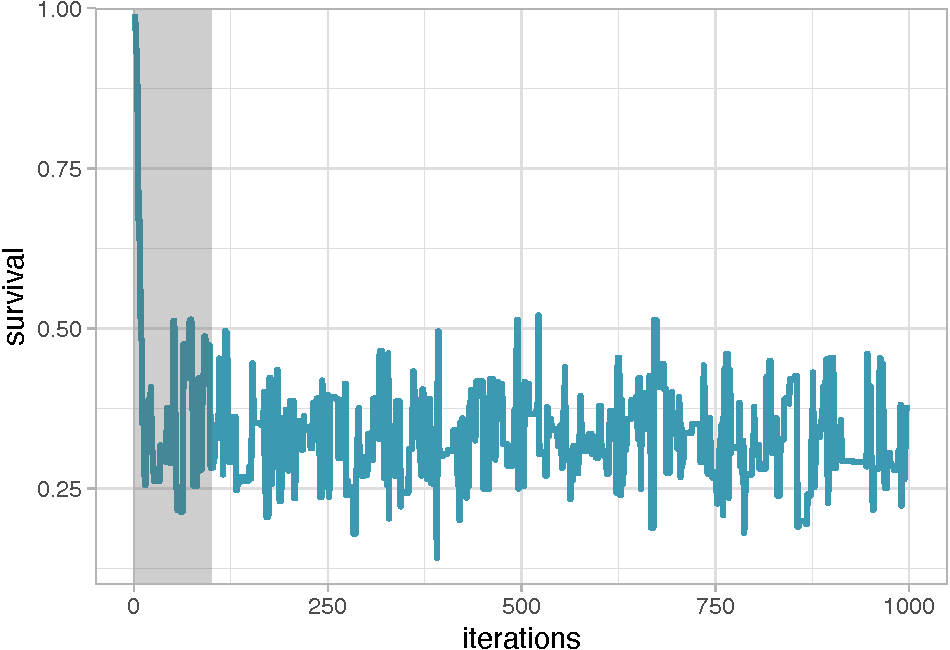
\includegraphics{banana-book_files/figure-latex/burnin-1.pdf}
\caption{\label{fig:burnin}Determining the length of the burn-in period. The chain starts at value 0.99 and rapidly stabilises, with values bouncing back and forth around 0.3 from the 100th iteration onwards. You may choose the shaded area as the burn-in, and discard the corresponding values.}
\end{figure}

Inspecting the trace plot for a single run of the Markov chain is useful. However, we usually run the Markov chain several times, starting from different over-dispersed points, to check that all runs achieve the same stationary distribution. This approach is formalised by using the Brooks-Gelman-Rubin (BGR) statistic \(\hat{R}\) which measures the ratio of the total variability combining multiple chains (between-chain plus within-chain) to the within-chain variability. The BGR statistic asks whether there is a chain effect, and is very much alike the \(F\) test in an analysis of variance. Values below 1.1 indicate likely convergence.

Back to our example, we run two Markov chains with starting values 0.2 and 0.8 using 100 up to 5000 iterations, and calculate the BGR statistic using half the number of iterations as the length of the burn-in. From Figure \ref{fig:bgr}, we get a value of the BGR statistic near 1 by up to 2000 iterations, which suggests that with 2000 iterations as a burn-in, there is no evidence of a lack of convergence.

\begin{figure}
\centering
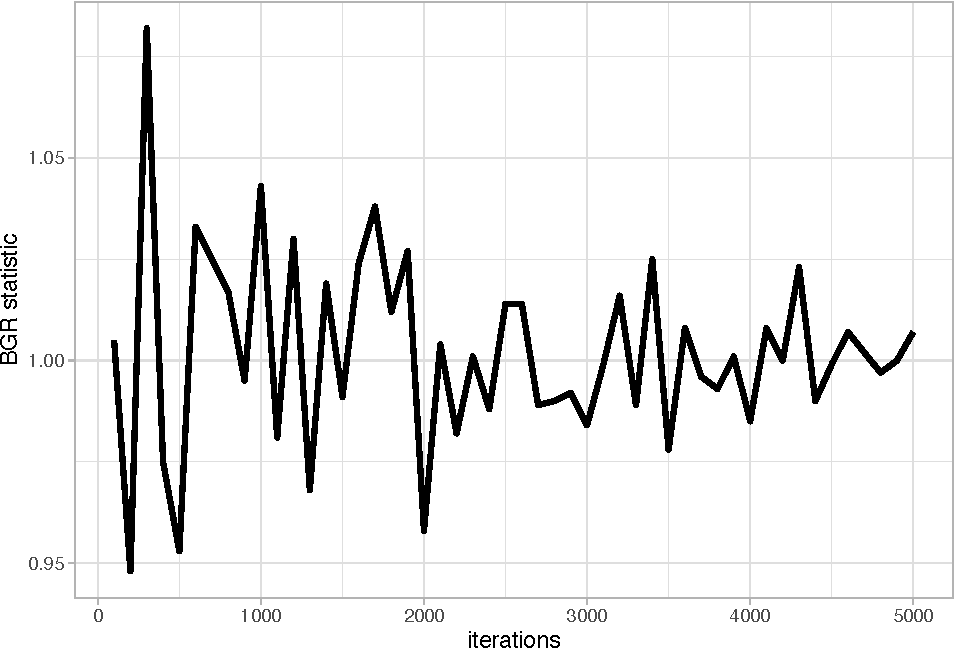
\includegraphics{banana-book_files/figure-latex/bgr-1.pdf}
\caption{\label{fig:bgr}Brooks-Gelman-Rubin statistic as a function of the number of iterations.}
\end{figure}

It is important to bear in mind that a value near 1 for the BGR statistic is only a necessary \emph{but not sufficient} condition for convergence. In other words, this diagnostic cannot tell you for sure that the Markov chain has achieved convergence, only that it has not.\footnote{Cross-reference sections on local minima and parameter redundancy for pathological cases.}

\hypertarget{chain-length}{%
\subsection{Chain length}\label{chain-length}}

How long of a chain is needed to produce reliable parameter estimates? To answer this question, you need to keep in mind that successive steps in a Markov chain are not independent -- this is usually referred to as \emph{autocorrelation}. Ideally, we would like to keep autocorrelation as low as possible. Here again, trace plots are useful to diagnose issues with autocorrelation. Let's get back to our survival example. Figure \ref{fig:tracechainlength} shows trace plots for different values of the standard deviation (parameter \emph{away}) of the (normal) proposal distribution we use to propose a candidate value (Section \ref{metropolis-algorithm}). Small and big moves provide high correlations between successive observations of the Markov chain, whereas a standard deviation of 1 allows efficient exploration of the parameter space. The movement around the parameter space is referred to as \emph{mixing}. Mixing is bad when the chain makes small and big moves, and good otherwise.

\begin{figure}
\centering
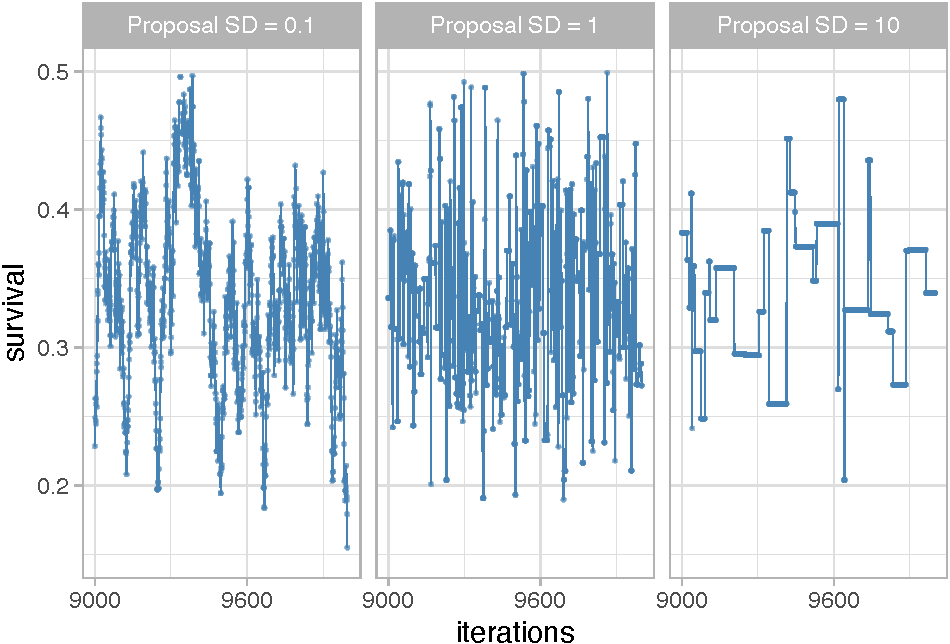
\includegraphics{banana-book_files/figure-latex/tracechainlength-1.pdf}
\caption{\label{fig:tracechainlength}Trace plots for different values of the standard deviation (SD) of the proposal distribution. Left: The chain exhibits small moves and mixing is bad. Right: The chain exhibits big moves and mixing is bad. Middle: The chain exhibits adequate moves and mixing is good. Only the thousand last iterations are shown.}
\end{figure}

In addition to trace plots, autocorrelation function (ACF) plots are a convenient way of displaying the strength of autocorrelation in a given sample values. ACF plots provide the autocorrelation between successively sampled values separated by an increasing number of iterations, or \emph{lag} (Figure \ref{fig:acfchainlength}).

\begin{figure}
\centering
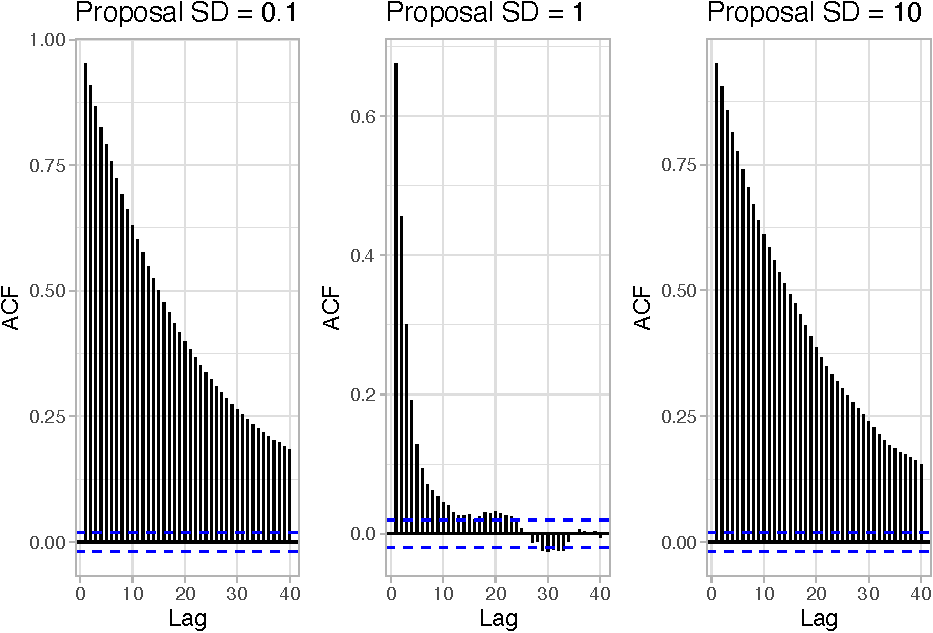
\includegraphics{banana-book_files/figure-latex/acfchainlength-1.pdf}
\caption{\label{fig:acfchainlength}Autocorrelation function plots for different values of the standard deviation (SD) of the proposal distribution. Left and right: Autocorrelation is strong, decreases slowly with increasing lag and mixing is bad. Middle: Autocorrelation is weak, decreases rapidly with increasing lag and mixing is good.}
\end{figure}

Autocorrelation is not necessarily a big issue. Strongly correlated observations just require large sample sizes and therefore longer simulations. But how many iterations exactly? The effective sample size (\texttt{n.eff}) measures chain length while taking into account chain autocorrelation. You should check the \texttt{n.eff} of every parameter of interest, and of any interesting parameter combinations. In general, we need \(\text{n.eff} \geq 1000\) independent steps to get reasonable Monte Carlo estimates of model parameters. In the animal survival example, \texttt{n.eff} can be calculated with the R \texttt{coda::effectiveSize()} function.

\begin{longtable}[]{@{}rr@{}}
\toprule
Proposal SD & n.eff \\
\midrule
\endhead
0.1 & 224 \\
1.0 & 1934 \\
10.0 & 230 \\
\bottomrule
\end{longtable}

As expected, \texttt{n.eff} is less than the number of MCMC iterations because of autocorrelation. Only when the standard deviation of the proposal distribution is 1 and mixing is good (Figures \ref{fig:tracechainlength} and \ref{fig:acfchainlength}) we get a satisfying effective sample size.

\hypertarget{what-if-you-have-issues-of-convergence}{%
\subsection{What if you have issues of convergence?}\label{what-if-you-have-issues-of-convergence}}

When diagnosing MCMC convergence, you will (very) often run into troubles. In this section you will find some helpful tips I hope.

When mixing is bad and effective sample size is small, you may just need to increase burn-in and/or sample more. Using more informative priors might also make Markov chains converge faster by helping your MCMC sampler (e.g.~the Metropolis algorithm) navigating more efficiently the parameter space. In the same spirit, picking better initial values for starting the chain does not harm. For doing that, a strategy consists in using estimates from a simpler model for which your MCMC chains do converge.

If convergence issues persist, often there is a problem with your model\footnote{The quote `When you have computational problems, often there's a problem with your model' is the folk theorem of statistical computing stated by Andrew Gelman in 2008, see \url{https://statmodeling.stat.columbia.edu/2008/05/13/the_folk_theore/}}. A bug in the code? A typo somewhere? A mistake in your maths? As often when coding is involved, the issue can be identified by removing complexities, and start with a simpler model until you find what the problem is.

A general advice is to see your model as a data generating tool in the first place, simulate data from it using some realistic values for the parameters, and try to recover these parameter values by fitting the model to the simulated data. Simulating from a model will help you understanding how it works, what it does not do, and the data you need to get reasonable parameter estimates.

We will see other strategies to improve convergence in the next chapters.\footnote{Cross reference relevant chapters. Option 1. Change your sampler. Option 2. Reparameterize (standardize covariates, plus non-centering: \(\alpha \sim N(0,\sigma)\) becomes \(\alpha = z \sigma\) with \(z \sim N(0,1)\)).}

\hypertarget{summary}{%
\section{Summary}\label{summary}}

\begin{itemize}
\item
  With the Bayes' theorem, you update your beliefs (prior) with new data (likelihood) to get posterior beliefs (posterior): posterior \(\propto\) likelihood \(\times\) prior.
\item
  The idea of Markov chain Monte Carlo (MCMC) is to simulate values from a Markov chain which has a stationary distribution equal to the posterior distribution you're after.
\item
  In practice, you run a Markov chain multiple times starting from over-dispersed initial values.
\item
  You discard iterations in an initial burn-in phase and achieve convergence when all chains reach the same regime.
\item
  From there, you run the chains long enough and proceed with calculating Monte Carlo estimates of numerical summaries (e.g.~posterior means and credible intervals) for parameters.
\end{itemize}

\hypertarget{suggested-reading}{%
\section{Suggested reading}\label{suggested-reading}}

\begin{itemize}
\item
  Gelman, A. and Hill, J. (2006). \href{https://www.cambridge.org/core/books/data-analysis-using-regression-and-multilevelhierarchical-models/32A29531C7FD730C3A68951A17C9D983}{Data Analysis Using Regression and Multilevel/Hierarchical Models (Analytical Methods for Social Research)}. Cambridge: Cambridge University Press.
\item
  Gelman, A. and colleagues (2020). \href{https://arxiv.org/pdf/2011.01808.pdf}{Bayesian workflow}. arXiv preprint.
\item
  McCarthy, M. (2007). \href{https://www.cambridge.org/core/books/bayesian-methods-for-ecology/9225F65B8A25D69B0B6C50B5A9A78201}{Bayesian Methods for Ecology}. Cambridge: Cambridge University Press.
\item
  McElreath, R. (2020). \href{https://xcelab.net/rm/statistical-rethinking/}{Statistical Rethinking: A Bayesian Course with Examples in R and Stan (2nd ed.)}. CRC Press.
\end{itemize}

\hypertarget{intronimble}{%
\chapter{NIMBLE tutorial}\label{intronimble}}

\hypertarget{introduction-2}{%
\section{Introduction}\label{introduction-2}}

In this second chapter, you will get familiar with NIMBLE, an R package that implements up-to-date MCMC algorithms for fitting complex models. NIMBLE spares you from coding the MCMC algorithms by hand, and requires only the specification of a likelihood and priors for model parameters. We will illustrate NIMBLE main features with a simple example, but the ideas hold for other problems.

\hypertarget{what-is-nimble}{%
\section{What is NIMBLE?}\label{what-is-nimble}}

NIMBLE stands for \textbf{N}umerical \textbf{I}nference for statistical \textbf{M}odels using \textbf{B}ayesian and \textbf{L}ikelihood \textbf{E}stimation. Briefly speaking, NIMBLE is an R package that implements for you MCMC algorithms to generate samples from the posterior distribution of model parameters. Freed from the burden of coding your own MCMC algorithms, you only have to specify a likelihood and priors to apply the Bayes theorem. To do so, NIMBLE uses a syntax very similar to the R syntax, which should make your life easier. This so-called BUGS language is also used by other programs like WinBUGS, OpenBUGS, and JAGS.

So why use NIMBLE you may ask? The short answer is that NIMBLE is capable of so much more than just running MCMC algorithms! First, you will work from within R, but in the background NIMBLE will translate your code in C++ for (in general) faster computation. Second, NIMBLE extends the BUGS language for writing new functions and distributions of your own, or borrow those written by others. Third, NIMBLE gives you full control of the MCMC samplers, and you may pick other algorithms than the defaults. Fourth, NIMBLE comes with a library of numerical methods other than MCMC algorithms, including sequential Monte Carlo (for particle filtering) and Monte Carlo Expectation Maximization (for maximum likelihood). Last but not least, the development team is friendly and helpful, and based on users' feedbacks, NIMBLE folks work constantly at improving the package capabilities.

\begin{figure}

{\centering 
\includegraphics[width=0.5\linewidth]{images/nimble-icon} 

}

\caption{Logo of the NIMBLE R package designed by Luke Larson. **Ask Perry for context and meaning.**}\label{fig:nimblelogo}
\end{figure}

\hypertarget{getting-started}{%
\section{Getting started}\label{getting-started}}

\begin{rmdnote}
To run NIMBLE, you will need to:\\
1. Build a model consisting of a likelihood and priors.\\
2. Read in some data.\\
3. Specify parameters you want to make inference about.\\
4. Pick initial values for parameters to be estimated (for each chain).\\
5. Provide MCMC details namely the number of chains, the length of the burn-in period and the number of iterations following burn-in.
\end{rmdnote}

First things first, let's not forget to load the \texttt{nimble} package:

\begin{Shaded}
\begin{Highlighting}[]
\FunctionTok{library}\NormalTok{(nimble)}
\end{Highlighting}
\end{Shaded}

Note that before you can install \texttt{nimble} like any other R package, Windows users will need to install \texttt{Rtools}, and Mac users will need to install \texttt{Xcode}. More at \url{https://r-nimble.org/download}.

Now let's go back to our example on animal survival from the previous chapter. First step is to build our model by specifying the binomial likelihood and a uniform prior on survival probability \texttt{theta}. We use the \texttt{nimbleCode()} function and wrap code within curly brackets:

\begin{Shaded}
\begin{Highlighting}[]
\NormalTok{model }\OtherTok{\textless{}{-}} \FunctionTok{nimbleCode}\NormalTok{(\{}
  \CommentTok{\# likelihood}
\NormalTok{  survived }\SpecialCharTok{\textasciitilde{}} \FunctionTok{dbinom}\NormalTok{(theta, released)}
  \CommentTok{\# prior}
\NormalTok{  theta }\SpecialCharTok{\textasciitilde{}} \FunctionTok{dunif}\NormalTok{(}\DecValTok{0}\NormalTok{, }\DecValTok{1}\NormalTok{)}
  \CommentTok{\# derived quantity}
\NormalTok{  lifespan }\OtherTok{\textless{}{-}} \SpecialCharTok{{-}}\DecValTok{1}\SpecialCharTok{/}\FunctionTok{log}\NormalTok{(theta)}
\NormalTok{\})}
\end{Highlighting}
\end{Shaded}

You can check that the \texttt{model} R object contains your code:

\begin{Shaded}
\begin{Highlighting}[]
\NormalTok{model}
\DocumentationTok{\#\# \{}
\DocumentationTok{\#\#     survived \textasciitilde{} dbinom(theta, released)}
\DocumentationTok{\#\#     theta \textasciitilde{} dunif(0, 1)}
\DocumentationTok{\#\#     lifespan \textless{}{-} {-}1/log(theta)}
\DocumentationTok{\#\# \}}
\end{Highlighting}
\end{Shaded}

In the code above, \texttt{survived} and \texttt{released} are known, only \texttt{theta} needs to be estimated. The line \texttt{survived\ \textasciitilde{}\ dbinom(theta,\ released)} states that the number of successes or animals that have survived over winter \texttt{survived} is distributed as (that's the \texttt{\textasciitilde{}}) as a binomial with \texttt{released} trials and probability of success or survival \texttt{theta}. Then the line \texttt{theta\ \textasciitilde{}\ dunif(0,\ 1)} assigns a uniform between 0 and 1 as a prior distribution to the survival probability. This is all you need, a likelihood and priors for model parameters, NIMBLE knows the Bayes theorem. The last line \texttt{lifespan\ \textless{}-\ -\ 1/log(theta)} calculates a quantity derived from \texttt{theta}, which is the expected lifespan assuming constant survival\footnote{Cook LM, Brower LP, Croze HJ (1967) The accuracy of a population estimation from multiple recapture data. J Anim Ecol 36:57--60}.

A few comments:

\begin{itemize}
\item
  The most common distributions are available in NIMBLE. Among others, we will use later in the book \texttt{dbeta}, \texttt{dmultinom} and \texttt{dnorm}. If you cannot find what you need in NIMBLE, you can write your own distribution as illustrated in Section \ref{functions-in-nimble}.
\item
  It does not matter in what order you write each line of code, NIMBLE uses what is called a declarative language for building models. In brief, you write code that tells NIMBLE what you want to achieve, and not how to get there. In contrast, an imperative language requires that you write what you want your program to do step by step.
\item
  You can think of models in NIMBLE as graphs as in Figure \ref{fig:dag-survival}. A graph is made of relations (or edges) that can be of two types. A stochastic relation is signaled by a \texttt{\textasciitilde{}} sign and defines a random variable in the model, such as \texttt{survived} or \texttt{theta}. A deterministic relation is signaled by a \texttt{\textless{}-} sign, like \texttt{lifespan}. Relations define nodes on the left - the children - in terms of other nodes on the right - the parents, and relations are directed edges from parents to children. Such graphs are called directed acyclic graph or DAG.
  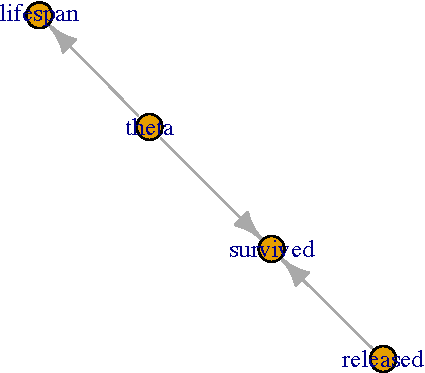
\includegraphics{banana-book_files/figure-latex/dag-survival-1.pdf}
\end{itemize}

Second step in our workflow is to read in some data. We use a list in which each component corresponds to a known quantity in the model:

\begin{Shaded}
\begin{Highlighting}[]
\NormalTok{my.data }\OtherTok{\textless{}{-}} \FunctionTok{list}\NormalTok{(}\AttributeTok{released =} \DecValTok{57}\NormalTok{, }\AttributeTok{survived =} \DecValTok{19}\NormalTok{)}
\end{Highlighting}
\end{Shaded}

You can proceed with data passed this way, but you should know a little more about how NIMBLE sees data. NIMBLE distinguishes data and constants. Constants are values that do not change, e.g.~vectors of known index values or the indices used to define for-loops. Data are values that you might want to change, basically anything that only appears on the left of a \texttt{\textasciitilde{}}. Declaring relevant values as constants is better for computational efficiency, but it is easy to forget, and fortunately NIMBLE will by itself distinguish data and constants. I will not use the distinction between data and constants in this chapter, but in the next chapters it will become important.

Third step is to tell NIMBLE which nodes in your model you would like to keep track of, in other words the quantities you'd like to do inference about. In our model we want survival \texttt{theta} and \texttt{lifespan}:

\begin{Shaded}
\begin{Highlighting}[]
\NormalTok{parameters.to.save }\OtherTok{\textless{}{-}} \FunctionTok{c}\NormalTok{(}\StringTok{"theta"}\NormalTok{, }\StringTok{"lifespan"}\NormalTok{)}
\end{Highlighting}
\end{Shaded}

In general you have many quantities in your model, including some of little interest that are not worth monitoring, and having full control on verbosity will prove handy.

Fourth step is to specify initial values for all model parameters. To make sure that the MCMC algorithm explores the posterior distribution, we start different chains with different parameter values. You can specify initial values for each chain in a list and put them in yet another list:

\begin{Shaded}
\begin{Highlighting}[]
\NormalTok{init1 }\OtherTok{\textless{}{-}} \FunctionTok{list}\NormalTok{(}\AttributeTok{theta =} \FloatTok{0.1}\NormalTok{)}
\NormalTok{init2 }\OtherTok{\textless{}{-}} \FunctionTok{list}\NormalTok{(}\AttributeTok{theta =} \FloatTok{0.5}\NormalTok{)}
\NormalTok{init3 }\OtherTok{\textless{}{-}} \FunctionTok{list}\NormalTok{(}\AttributeTok{theta =} \FloatTok{0.9}\NormalTok{)}
\NormalTok{initial.values }\OtherTok{\textless{}{-}} \FunctionTok{list}\NormalTok{(init1, init2, init3)}
\NormalTok{initial.values}
\DocumentationTok{\#\# [[1]]}
\DocumentationTok{\#\# [[1]]$theta}
\DocumentationTok{\#\# [1] 0.1}
\DocumentationTok{\#\# }
\DocumentationTok{\#\# }
\DocumentationTok{\#\# [[2]]}
\DocumentationTok{\#\# [[2]]$theta}
\DocumentationTok{\#\# [1] 0.5}
\DocumentationTok{\#\# }
\DocumentationTok{\#\# }
\DocumentationTok{\#\# [[3]]}
\DocumentationTok{\#\# [[3]]$theta}
\DocumentationTok{\#\# [1] 0.9}
\end{Highlighting}
\end{Shaded}

Alternatively, you can write a simple R function that generates random initial values:

\begin{Shaded}
\begin{Highlighting}[]
\NormalTok{initial.values }\OtherTok{\textless{}{-}} \ControlFlowTok{function}\NormalTok{() }\FunctionTok{list}\NormalTok{(}\AttributeTok{theta =} \FunctionTok{runif}\NormalTok{(}\DecValTok{1}\NormalTok{,}\DecValTok{0}\NormalTok{,}\DecValTok{1}\NormalTok{))}
\FunctionTok{initial.values}\NormalTok{()}
\DocumentationTok{\#\# $theta}
\DocumentationTok{\#\# [1] 0.1146}
\end{Highlighting}
\end{Shaded}

Firth and last step, you need to tell NIMBLE the number of chains to run, say \texttt{n.chain}, how long the burn-in period should be, say \texttt{n.burnin}, and the number of iterations following the burn-in period to be used for posterior inference. In NIMBLE, you specify the total number of iterations, say \texttt{n.iter}, so that the number of posterior samples per chain is \texttt{n.iter\ -\ n.burnin}. NIMBLE also allows discarding samples after burn-in, a procedure known as thinning, which I will not use in this book\footnote{Link, W.A. and Eaton, M.J. (2012), On thinning of chains in MCMC. Methods in Ecology and Evolution, 3: 112-115.}.

\begin{Shaded}
\begin{Highlighting}[]
\NormalTok{n.iter }\OtherTok{\textless{}{-}} \DecValTok{5000}
\NormalTok{n.burnin }\OtherTok{\textless{}{-}} \DecValTok{1000}
\NormalTok{n.chains }\OtherTok{\textless{}{-}} \DecValTok{3}
\end{Highlighting}
\end{Shaded}

We now have all the ingredients to run model, that is to sample in the posterior distribution of model parameters using MCMC simulations. This is accomplished using function \texttt{nimbleMCMC()}:

\begin{Shaded}
\begin{Highlighting}[]
\NormalTok{mcmc.output }\OtherTok{\textless{}{-}} \FunctionTok{nimbleMCMC}\NormalTok{(}\AttributeTok{code =}\NormalTok{ model,}
                          \AttributeTok{data =}\NormalTok{ my.data,}
                          \AttributeTok{inits =}\NormalTok{ initial.values,}
                          \AttributeTok{monitors =}\NormalTok{ parameters.to.save,}
                          \AttributeTok{niter =}\NormalTok{ n.iter,}
                          \AttributeTok{nburnin =}\NormalTok{ n.burnin,}
                          \AttributeTok{nchains =}\NormalTok{ n.chains)}
\DocumentationTok{\#\# |{-}{-}{-}{-}{-}{-}{-}{-}{-}{-}{-}{-}{-}|{-}{-}{-}{-}{-}{-}{-}{-}{-}{-}{-}{-}{-}|{-}{-}{-}{-}{-}{-}{-}{-}{-}{-}{-}{-}{-}|{-}{-}{-}{-}{-}{-}{-}{-}{-}{-}{-}{-}{-}|}
\DocumentationTok{\#\# |{-}{-}{-}{-}{-}{-}{-}{-}{-}{-}{-}{-}{-}{-}{-}{-}{-}{-}{-}{-}{-}{-}{-}{-}{-}{-}{-}{-}{-}{-}{-}{-}{-}{-}{-}{-}{-}{-}{-}{-}{-}{-}{-}{-}{-}{-}{-}{-}{-}{-}{-}{-}{-}{-}{-}|}
\DocumentationTok{\#\# |{-}{-}{-}{-}{-}{-}{-}{-}{-}{-}{-}{-}{-}|{-}{-}{-}{-}{-}{-}{-}{-}{-}{-}{-}{-}{-}|{-}{-}{-}{-}{-}{-}{-}{-}{-}{-}{-}{-}{-}|{-}{-}{-}{-}{-}{-}{-}{-}{-}{-}{-}{-}{-}|}
\DocumentationTok{\#\# |{-}{-}{-}{-}{-}{-}{-}{-}{-}{-}{-}{-}{-}{-}{-}{-}{-}{-}{-}{-}{-}{-}{-}{-}{-}{-}{-}{-}{-}{-}{-}{-}{-}{-}{-}{-}{-}{-}{-}{-}{-}{-}{-}{-}{-}{-}{-}{-}{-}{-}{-}{-}{-}{-}{-}|}
\DocumentationTok{\#\# |{-}{-}{-}{-}{-}{-}{-}{-}{-}{-}{-}{-}{-}|{-}{-}{-}{-}{-}{-}{-}{-}{-}{-}{-}{-}{-}|{-}{-}{-}{-}{-}{-}{-}{-}{-}{-}{-}{-}{-}|{-}{-}{-}{-}{-}{-}{-}{-}{-}{-}{-}{-}{-}|}
\DocumentationTok{\#\# |{-}{-}{-}{-}{-}{-}{-}{-}{-}{-}{-}{-}{-}{-}{-}{-}{-}{-}{-}{-}{-}{-}{-}{-}{-}{-}{-}{-}{-}{-}{-}{-}{-}{-}{-}{-}{-}{-}{-}{-}{-}{-}{-}{-}{-}{-}{-}{-}{-}{-}{-}{-}{-}{-}{-}|}
\end{Highlighting}
\end{Shaded}

NIMBLE goes through several steps that we will explain in Section \ref{under-the-hood}. Function \texttt{nimbleMCMC()} takes other arguments that you might find useful. For example, you can suppress the progress bar if you find it to depressing when running long simulations with \texttt{progressBar\ =\ FALSE}. You can also get a summary of the outputs by specifying \texttt{summary\ =\ TRUE}. Check \texttt{?nimbleMCMC} for more details.

Now let's inspect what we have in \texttt{mcmc.output}.

\begin{Shaded}
\begin{Highlighting}[]
\FunctionTok{str}\NormalTok{(mcmc.output)}
\DocumentationTok{\#\# List of 3}
\DocumentationTok{\#\#  $ chain1: num [1:4000, 1:2] 0.814 0.814 1.024 1.024 0.964 ...}
\DocumentationTok{\#\#   ..{-} attr(*, "dimnames")=List of 2}
\DocumentationTok{\#\#   .. ..$ : NULL}
\DocumentationTok{\#\#   .. ..$ : chr [1:2] "lifespan" "theta"}
\DocumentationTok{\#\#  $ chain2: num [1:4000, 1:2] 0.852 0.852 0.801 0.902 0.902 ...}
\DocumentationTok{\#\#   ..{-} attr(*, "dimnames")=List of 2}
\DocumentationTok{\#\#   .. ..$ : NULL}
\DocumentationTok{\#\#   .. ..$ : chr [1:2] "lifespan" "theta"}
\DocumentationTok{\#\#  $ chain3: num [1:4000, 1:2] 0.836 1.098 1.098 1.098 0.856 ...}
\DocumentationTok{\#\#   ..{-} attr(*, "dimnames")=List of 2}
\DocumentationTok{\#\#   .. ..$ : NULL}
\DocumentationTok{\#\#   .. ..$ : chr [1:2] "lifespan" "theta"}
\end{Highlighting}
\end{Shaded}

The R object \texttt{mcmc.output} is a list with three components, one for each MCMC chain. Let's have a look to \texttt{chain1} for example.

\begin{Shaded}
\begin{Highlighting}[]
\FunctionTok{dim}\NormalTok{(mcmc.output}\SpecialCharTok{$}\NormalTok{chain1)}
\DocumentationTok{\#\# [1] 4000    2}
\FunctionTok{head}\NormalTok{(mcmc.output}\SpecialCharTok{$}\NormalTok{chain1)}
\DocumentationTok{\#\#      lifespan  theta}
\DocumentationTok{\#\# [1,]   0.8140 0.2928}
\DocumentationTok{\#\# [2,]   0.8140 0.2928}
\DocumentationTok{\#\# [3,]   1.0236 0.3764}
\DocumentationTok{\#\# [4,]   1.0236 0.3764}
\DocumentationTok{\#\# [5,]   0.9636 0.3542}
\DocumentationTok{\#\# [6,]   0.9636 0.3542}
\end{Highlighting}
\end{Shaded}

Each component of the list is a matrix. In rows, you have 4000 samples from the posterior distribution of \texttt{theta}, which corresponds to \texttt{n.iter\ -\ n.burnin} iterations. In columns, you have the quantities we monitor, \texttt{theta} and \texttt{lifespan}. From there, you can compute the posterior mean of \texttt{theta}:

\begin{Shaded}
\begin{Highlighting}[]
\FunctionTok{mean}\NormalTok{(mcmc.output}\SpecialCharTok{$}\NormalTok{chain1[,}\StringTok{\textquotesingle{}theta\textquotesingle{}}\NormalTok{])}
\DocumentationTok{\#\# [1] 0.3388}
\end{Highlighting}
\end{Shaded}

You can also obtain the 95\% credible interval for \texttt{theta}:

\begin{Shaded}
\begin{Highlighting}[]
\FunctionTok{quantile}\NormalTok{(mcmc.output}\SpecialCharTok{$}\NormalTok{chain1[,}\StringTok{\textquotesingle{}theta\textquotesingle{}}\NormalTok{], }\AttributeTok{probs =} \FunctionTok{c}\NormalTok{(}\FloatTok{2.5}\NormalTok{, }\FloatTok{97.5}\NormalTok{)}\SpecialCharTok{/}\DecValTok{100}\NormalTok{)}
\DocumentationTok{\#\#   2.5\%  97.5\% }
\DocumentationTok{\#\# 0.2211 0.4659}
\end{Highlighting}
\end{Shaded}

Let's visualise the posterior distribution of \texttt{theta} with a histogram:

\begin{Shaded}
\begin{Highlighting}[]
\NormalTok{mcmc.output }\SpecialCharTok{\%\textgreater{}\%}
  \FunctionTok{as\_tibble}\NormalTok{() }\SpecialCharTok{\%\textgreater{}\%}
  \FunctionTok{ggplot}\NormalTok{() }\SpecialCharTok{+}
  \FunctionTok{geom\_histogram}\NormalTok{(}\FunctionTok{aes}\NormalTok{(}\AttributeTok{x =}\NormalTok{ chain1[,}\StringTok{"theta"}\NormalTok{]), }\AttributeTok{color =} \StringTok{"white"}\NormalTok{) }\SpecialCharTok{+}
  \FunctionTok{labs}\NormalTok{(}\AttributeTok{x =} \StringTok{"survival probability"}\NormalTok{)}
\end{Highlighting}
\end{Shaded}

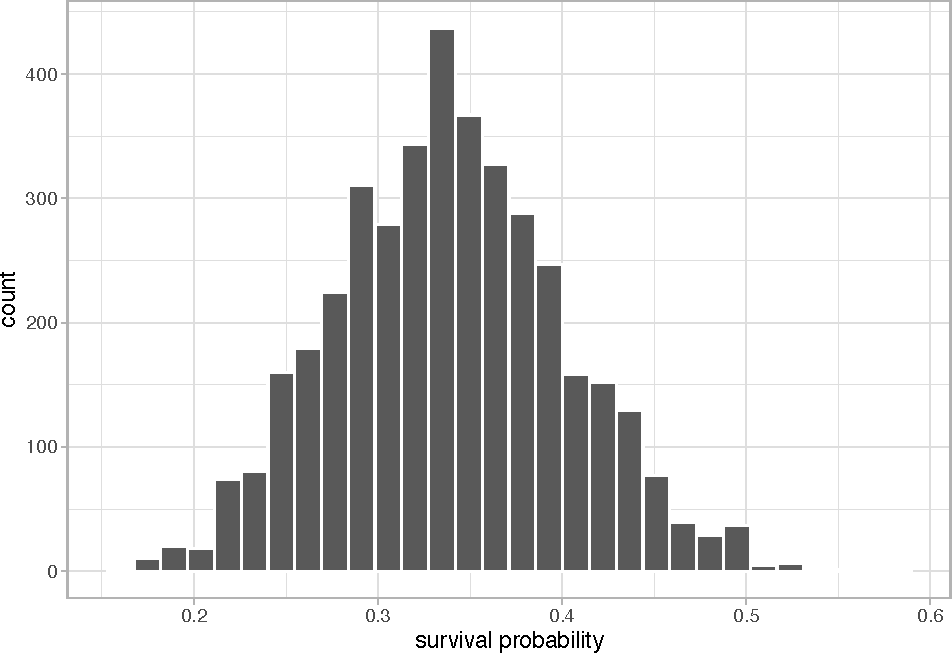
\includegraphics{banana-book_files/figure-latex/unnamed-chunk-43-1.pdf}

There are less painful ways of doing posterior inference. In this book, I will use the R package \texttt{MCMCvis}\footnote{\url{https://github.com/caseyyoungflesh/MCMCvis}} to summarise and visualize MCMC outputs, but there are other perfectly valid options out there like \texttt{ggmcmc}\footnote{Fernández-i-Marín, X. (2016). ggmcmc: Analysis of MCMC Samples and Bayesian Inference. Journal of Statistical Software, 70(9), 1--20} and \texttt{basicMCMCplots}\footnote{\url{https://cran.r-project.org/web/packages/basicMCMCplots/index.html}}. \textbf{Shall I demonstrate these other options?}

Let's load the package \texttt{MCMCvis}:

\begin{Shaded}
\begin{Highlighting}[]
\FunctionTok{library}\NormalTok{(MCMCvis)}
\end{Highlighting}
\end{Shaded}

To get the most common numerical summaries, the function \texttt{MCMCsummary()} does the job:

\begin{Shaded}
\begin{Highlighting}[]
\FunctionTok{MCMCsummary}\NormalTok{(}\AttributeTok{object =}\NormalTok{ mcmc.output, }\AttributeTok{round =} \DecValTok{2}\NormalTok{)}
\DocumentationTok{\#\#          mean   sd 2.5\%  50\% 97.5\% Rhat n.eff}
\DocumentationTok{\#\# lifespan 0.94 0.16 0.67 0.92  1.32    1  2545}
\DocumentationTok{\#\# theta    0.34 0.06 0.22 0.34  0.47    1  2675}
\end{Highlighting}
\end{Shaded}

You can use a caterpillar plot to visualise the posterior distributions of \texttt{theta} with \texttt{MCMCplot()}:

\begin{Shaded}
\begin{Highlighting}[]
\FunctionTok{MCMCplot}\NormalTok{(}\AttributeTok{object =}\NormalTok{ mcmc.output, }
         \AttributeTok{params =} \StringTok{\textquotesingle{}theta\textquotesingle{}}\NormalTok{)}
\end{Highlighting}
\end{Shaded}

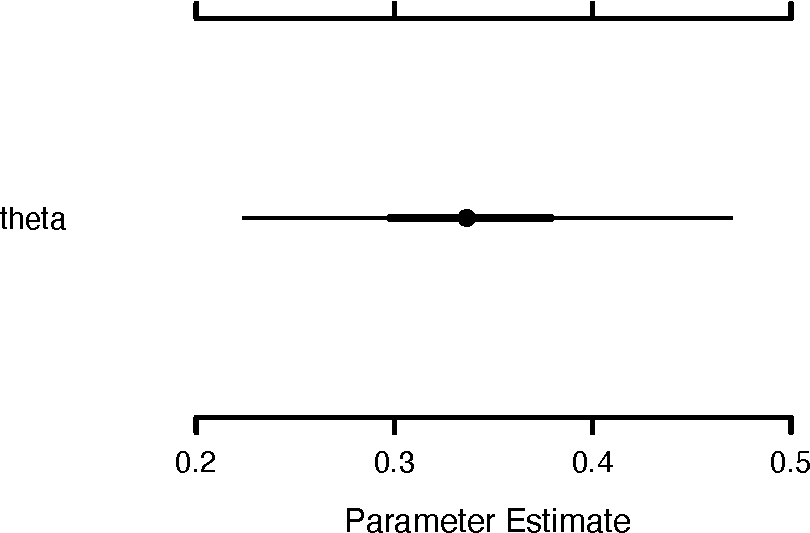
\includegraphics{banana-book_files/figure-latex/unnamed-chunk-46-1.pdf}

The point represents the posterior median, the thick line is the 50\% credible interval and the thin line the 95\% credible interval.

The trace and posterior density of theta can be obtained with \texttt{MCMCtrace()}:

\begin{Shaded}
\begin{Highlighting}[]
\FunctionTok{MCMCtrace}\NormalTok{(}\AttributeTok{object =}\NormalTok{ mcmc.output,}
          \AttributeTok{pdf =} \ConstantTok{FALSE}\NormalTok{, }\CommentTok{\# no export to PDF}
          \AttributeTok{ind =} \ConstantTok{TRUE}\NormalTok{, }\CommentTok{\# separate density lines per chain}
          \AttributeTok{params =} \StringTok{"theta"}\NormalTok{)}
\end{Highlighting}
\end{Shaded}

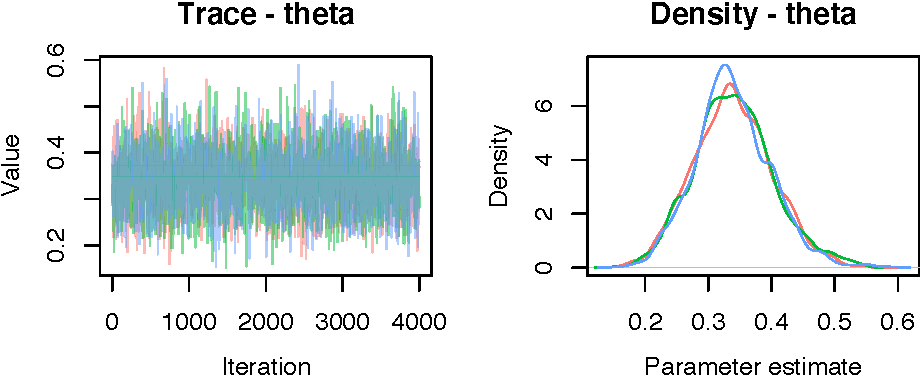
\includegraphics{banana-book_files/figure-latex/unnamed-chunk-47-1.pdf}

You can also add the diagnostics of convergence we discussed in the previous chapter:

\begin{Shaded}
\begin{Highlighting}[]
\FunctionTok{MCMCtrace}\NormalTok{(}\AttributeTok{object =}\NormalTok{ mcmc.output,}
          \AttributeTok{pdf =} \ConstantTok{FALSE}\NormalTok{,}
          \AttributeTok{ind =} \ConstantTok{TRUE}\NormalTok{,}
          \AttributeTok{Rhat =} \ConstantTok{TRUE}\NormalTok{, }\CommentTok{\# add Rhat}
          \AttributeTok{n.eff =} \ConstantTok{TRUE}\NormalTok{, }\CommentTok{\# add eff sample size}
          \AttributeTok{params =} \StringTok{"theta"}\NormalTok{)}
\end{Highlighting}
\end{Shaded}

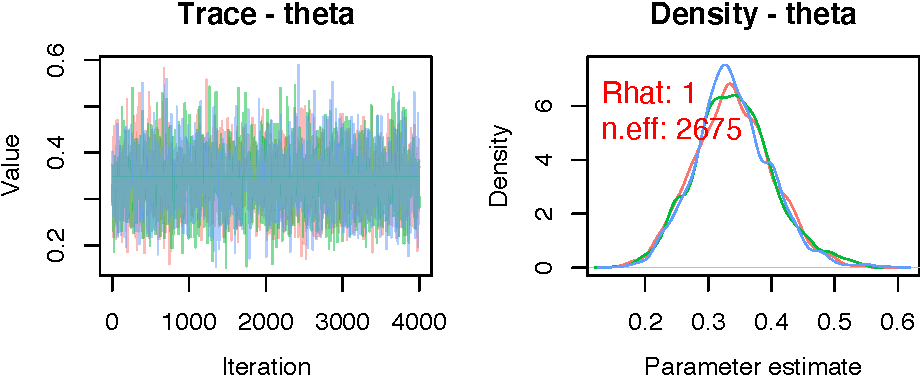
\includegraphics{banana-book_files/figure-latex/unnamed-chunk-48-1.pdf}

We calculated lifespan directly in our model with \texttt{lifespan\ \textless{}-\ -1/log(theta)}. But you can also calculate this quantity from outside NIMBLE. This is a nice by-product of using MCMC simulations: you can obtain the posterior distribution of any quantity that is function of your model parameters by applying this function to samples from the posterior distribution of these parameters. In our example, all you need is samples from the posterior distribution of \texttt{theta}, which we pool between the three chains with:

\begin{Shaded}
\begin{Highlighting}[]
\NormalTok{theta\_samples }\OtherTok{\textless{}{-}} \FunctionTok{c}\NormalTok{(mcmc.output}\SpecialCharTok{$}\NormalTok{chain1[,}\StringTok{\textquotesingle{}theta\textquotesingle{}}\NormalTok{], }
\NormalTok{                   mcmc.output}\SpecialCharTok{$}\NormalTok{chain2[,}\StringTok{\textquotesingle{}theta\textquotesingle{}}\NormalTok{],}
\NormalTok{                   mcmc.output}\SpecialCharTok{$}\NormalTok{chain3[,}\StringTok{\textquotesingle{}theta\textquotesingle{}}\NormalTok{])}
\end{Highlighting}
\end{Shaded}

To get samples from the posterior distribution of lifespan, we apply the function to calculate lifespan to the samples from the posterior distribution of survival:

\begin{Shaded}
\begin{Highlighting}[]
\NormalTok{lifespan }\OtherTok{\textless{}{-}} \SpecialCharTok{{-}}\DecValTok{1}\SpecialCharTok{/}\FunctionTok{log}\NormalTok{(theta\_samples)}
\end{Highlighting}
\end{Shaded}

As usual then, you can calculate the posterior mean and 95\% credible interval:

\begin{Shaded}
\begin{Highlighting}[]
\FunctionTok{mean}\NormalTok{(lifespan)}
\DocumentationTok{\#\# [1] 0.9385}
\FunctionTok{quantile}\NormalTok{(lifespan, }\AttributeTok{probs =} \FunctionTok{c}\NormalTok{(}\FloatTok{2.5}\NormalTok{, }\FloatTok{97.5}\NormalTok{)}\SpecialCharTok{/}\DecValTok{100}\NormalTok{)}
\DocumentationTok{\#\#   2.5\%  97.5\% }
\DocumentationTok{\#\# 0.6684 1.3243}
\end{Highlighting}
\end{Shaded}

You can also visualise the posterior distribution of lifespan:

\begin{Shaded}
\begin{Highlighting}[]
\NormalTok{lifespan }\SpecialCharTok{\%\textgreater{}\%}
  \FunctionTok{as\_tibble}\NormalTok{() }\SpecialCharTok{\%\textgreater{}\%}
  \FunctionTok{ggplot}\NormalTok{() }\SpecialCharTok{+}
  \FunctionTok{geom\_histogram}\NormalTok{(}\FunctionTok{aes}\NormalTok{(}\AttributeTok{x =}\NormalTok{ value), }\AttributeTok{color =} \StringTok{"white"}\NormalTok{) }\SpecialCharTok{+}
  \FunctionTok{labs}\NormalTok{(}\AttributeTok{x =} \StringTok{"lifespan"}\NormalTok{)}
\end{Highlighting}
\end{Shaded}

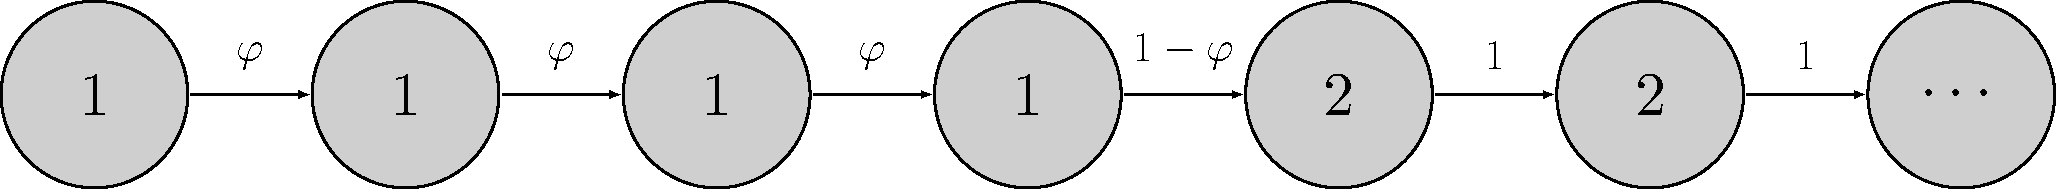
\includegraphics{banana-book_files/figure-latex/unnamed-chunk-52-1.pdf}

Now you're good to go. The NIMBLE workflow provided with \texttt{nimbleMCMC()} allows you to build models and make inference. This is what you can achieve with other software like WinBUGS or JAGS.

But NIMBLE is more than just another MCMC engine. It provides a programming environment so that you have full control when building models and estimating parameters. NIMBLE allows you to write your own functions and distributions to build models, and to choose alternative MCMC samplers or code new ones. This flexibility often comes with faster convergence.

I have to be honest, learning these improvements over other software takes some reading and experimentation, and it might well be that you do not need to use any of these features. And it's fine. In the next sections, I cover some of this advanced material. You may skip these sections and go back to this material later if you need it.

\hypertarget{functions-in-nimble}{%
\section{Functions in NIMBLE}\label{functions-in-nimble}}

In NIMBLE you can write and use your own functions, or use existing R or C/C++ functions. This allows you to customize models the way you want.

\hypertarget{write-nimblefunctions}{%
\subsection{Write nimbleFunctions}\label{write-nimblefunctions}}

NIMBLE provides \texttt{nimbleFunctions} for programming. A \texttt{nimbleFunction} is like an R function, plus it can be compiled for faster computation. Going back to our animal survival example, we can write a \texttt{nimbleFunction} to compute lifespan:

\begin{Shaded}
\begin{Highlighting}[]
\NormalTok{computeLifespan }\OtherTok{\textless{}{-}} \FunctionTok{nimbleFunction}\NormalTok{(}
    \AttributeTok{run =} \ControlFlowTok{function}\NormalTok{(}\AttributeTok{theta =} \FunctionTok{double}\NormalTok{(}\DecValTok{0}\NormalTok{)) \{ }\CommentTok{\# type declarations}
\NormalTok{        ans }\OtherTok{\textless{}{-}} \SpecialCharTok{{-}}\DecValTok{1}\SpecialCharTok{/}\FunctionTok{log}\NormalTok{(theta)}
        \FunctionTok{return}\NormalTok{(ans)}
        \FunctionTok{returnType}\NormalTok{(}\FunctionTok{double}\NormalTok{(}\DecValTok{0}\NormalTok{))  }\CommentTok{\# return type declaration}
\NormalTok{    \} )}
\end{Highlighting}
\end{Shaded}

Within the nimbleFunction, the \texttt{run} section gives the function to be executed. It is written in the NIMBLE language. The \texttt{theta\ =\ double(0)} and \texttt{returnType(double(0))} arguments tell NIMBLE that the input and output are single numeric values (scalars). Alternatively, \texttt{double(1)} and \texttt{double(2)} are for vectors and matrices, while \texttt{logical()}, \texttt{integer()} and \texttt{character()} are for logical, integer and character values.

You can use your \texttt{nimbleFunction} in R:

\begin{Shaded}
\begin{Highlighting}[]
\FunctionTok{computeLifespan}\NormalTok{(}\FloatTok{0.8}\NormalTok{)}
\DocumentationTok{\#\# [1] 4.481}
\end{Highlighting}
\end{Shaded}

You can compile it and use the C++ code for faster computation:

\begin{Shaded}
\begin{Highlighting}[]
\NormalTok{CcomputeLifespan }\OtherTok{\textless{}{-}} \FunctionTok{compileNimble}\NormalTok{(computeLifespan)}
\FunctionTok{CcomputeLifespan}\NormalTok{(}\FloatTok{0.8}\NormalTok{)}
\DocumentationTok{\#\# [1] 4.481}
\end{Highlighting}
\end{Shaded}

You can also use your \texttt{nimbleFunction} in a model:

\begin{Shaded}
\begin{Highlighting}[]
\NormalTok{model }\OtherTok{\textless{}{-}} \FunctionTok{nimbleCode}\NormalTok{(\{}
  \CommentTok{\# likelihood}
\NormalTok{  survived }\SpecialCharTok{\textasciitilde{}} \FunctionTok{dbinom}\NormalTok{(theta, released)}
  \CommentTok{\# prior}
\NormalTok{  theta }\SpecialCharTok{\textasciitilde{}} \FunctionTok{dunif}\NormalTok{(}\DecValTok{0}\NormalTok{, }\DecValTok{1}\NormalTok{)}
  \CommentTok{\# derived quantity}
\NormalTok{  lifespan }\OtherTok{\textless{}{-}} \FunctionTok{computeLifespan}\NormalTok{(theta)}
\NormalTok{\})}
\end{Highlighting}
\end{Shaded}

The rest of the workflow remains the same:

\begin{Shaded}
\begin{Highlighting}[]
\NormalTok{my.data }\OtherTok{\textless{}{-}} \FunctionTok{list}\NormalTok{(}\AttributeTok{survived =} \DecValTok{19}\NormalTok{, }\AttributeTok{released =} \DecValTok{57}\NormalTok{)}
\NormalTok{parameters.to.save }\OtherTok{\textless{}{-}} \FunctionTok{c}\NormalTok{(}\StringTok{"theta"}\NormalTok{, }\StringTok{"lifespan"}\NormalTok{)}
\NormalTok{initial.values }\OtherTok{\textless{}{-}} \ControlFlowTok{function}\NormalTok{() }\FunctionTok{list}\NormalTok{(}\AttributeTok{theta =} \FunctionTok{runif}\NormalTok{(}\DecValTok{1}\NormalTok{,}\DecValTok{0}\NormalTok{,}\DecValTok{1}\NormalTok{))}
\NormalTok{n.iter }\OtherTok{\textless{}{-}} \DecValTok{5000}
\NormalTok{n.burnin }\OtherTok{\textless{}{-}} \DecValTok{1000}
\NormalTok{n.chains }\OtherTok{\textless{}{-}} \DecValTok{3}
\NormalTok{mcmc.output }\OtherTok{\textless{}{-}} \FunctionTok{nimbleMCMC}\NormalTok{(}\AttributeTok{code =}\NormalTok{ model,}
                          \AttributeTok{data =}\NormalTok{ my.data,}
                          \AttributeTok{inits =}\NormalTok{ initial.values,}
                          \AttributeTok{monitors =}\NormalTok{ parameters.to.save,}
                          \AttributeTok{niter =}\NormalTok{ n.iter,}
                          \AttributeTok{nburnin =}\NormalTok{ n.burnin,}
                          \AttributeTok{nchains =}\NormalTok{ n.chains)}
\DocumentationTok{\#\# |{-}{-}{-}{-}{-}{-}{-}{-}{-}{-}{-}{-}{-}|{-}{-}{-}{-}{-}{-}{-}{-}{-}{-}{-}{-}{-}|{-}{-}{-}{-}{-}{-}{-}{-}{-}{-}{-}{-}{-}|{-}{-}{-}{-}{-}{-}{-}{-}{-}{-}{-}{-}{-}|}
\DocumentationTok{\#\# |{-}{-}{-}{-}{-}{-}{-}{-}{-}{-}{-}{-}{-}{-}{-}{-}{-}{-}{-}{-}{-}{-}{-}{-}{-}{-}{-}{-}{-}{-}{-}{-}{-}{-}{-}{-}{-}{-}{-}{-}{-}{-}{-}{-}{-}{-}{-}{-}{-}{-}{-}{-}{-}{-}{-}|}
\DocumentationTok{\#\# |{-}{-}{-}{-}{-}{-}{-}{-}{-}{-}{-}{-}{-}|{-}{-}{-}{-}{-}{-}{-}{-}{-}{-}{-}{-}{-}|{-}{-}{-}{-}{-}{-}{-}{-}{-}{-}{-}{-}{-}|{-}{-}{-}{-}{-}{-}{-}{-}{-}{-}{-}{-}{-}|}
\DocumentationTok{\#\# |{-}{-}{-}{-}{-}{-}{-}{-}{-}{-}{-}{-}{-}{-}{-}{-}{-}{-}{-}{-}{-}{-}{-}{-}{-}{-}{-}{-}{-}{-}{-}{-}{-}{-}{-}{-}{-}{-}{-}{-}{-}{-}{-}{-}{-}{-}{-}{-}{-}{-}{-}{-}{-}{-}{-}|}
\DocumentationTok{\#\# |{-}{-}{-}{-}{-}{-}{-}{-}{-}{-}{-}{-}{-}|{-}{-}{-}{-}{-}{-}{-}{-}{-}{-}{-}{-}{-}|{-}{-}{-}{-}{-}{-}{-}{-}{-}{-}{-}{-}{-}|{-}{-}{-}{-}{-}{-}{-}{-}{-}{-}{-}{-}{-}|}
\DocumentationTok{\#\# |{-}{-}{-}{-}{-}{-}{-}{-}{-}{-}{-}{-}{-}{-}{-}{-}{-}{-}{-}{-}{-}{-}{-}{-}{-}{-}{-}{-}{-}{-}{-}{-}{-}{-}{-}{-}{-}{-}{-}{-}{-}{-}{-}{-}{-}{-}{-}{-}{-}{-}{-}{-}{-}{-}{-}|}
\FunctionTok{MCMCsummary}\NormalTok{(}\AttributeTok{object =}\NormalTok{ mcmc.output, }\AttributeTok{round =} \DecValTok{2}\NormalTok{)}
\DocumentationTok{\#\#          mean   sd 2.5\%  50\% 97.5\% Rhat n.eff}
\DocumentationTok{\#\# lifespan 0.93 0.16 0.67 0.92  1.28    1  2756}
\DocumentationTok{\#\# theta    0.34 0.06 0.22 0.34  0.46    1  2781}
\end{Highlighting}
\end{Shaded}

With \texttt{nimbleFunctions}, you can mimic basic R syntax, do linear algebra (e.g.~compute eigenvalues), operate on vectors and matrices (e.g.~inverse a matrix), use logical operators (e.g.~and/or) and flow control (e.g.~if-else). There is also a long list of common and less common distributions that can be used with \texttt{nimbleFunctions}.

To learn everything you need to know on writing \texttt{nimbleFunctions}, make sure to read chapter 11 of the NIMBLE manual at \url{https://r-nimble.org/html_manual/cha-RCfunctions.html\#cha-RCfunctions}.

\hypertarget{call-existing-rc-functions-from-nimble}{%
\subsection{Call existing R/C++ functions from NIMBLE}\label{call-existing-rc-functions-from-nimble}}

If you're like me, and too lazy to write your own functions, you can rely on the scientific community and use existing C, C++ or R code. The trick is to write a \texttt{nimbleFunction} that wraps access to that code which can then be used by NIMBLE. As an example, imagine you'd like to use an R function \texttt{myfunction()}, either a function you wrote yourself, or a function available in your favorite R package:

\begin{Shaded}
\begin{Highlighting}[]
\NormalTok{myfunction }\OtherTok{\textless{}{-}} \ControlFlowTok{function}\NormalTok{(x) \{}
  \SpecialCharTok{{-}}\DecValTok{1}\SpecialCharTok{/}\FunctionTok{log}\NormalTok{(x)}
\NormalTok{\}}
\end{Highlighting}
\end{Shaded}

Now wrap this function using \texttt{nimbleRcall()} or \texttt{nimbleExternalCall()} for a C or C++ function:

\begin{Shaded}
\begin{Highlighting}[]
\NormalTok{Rmyfunction }\OtherTok{\textless{}{-}} \FunctionTok{nimbleRcall}\NormalTok{(}\AttributeTok{prototype =} \ControlFlowTok{function}\NormalTok{(}\AttributeTok{x =} \FunctionTok{double}\NormalTok{(}\DecValTok{0}\NormalTok{))\{\}, }
                           \AttributeTok{Rfun =} \StringTok{\textquotesingle{}myfunction\textquotesingle{}}\NormalTok{,}
                           \AttributeTok{returnType =} \FunctionTok{double}\NormalTok{(}\DecValTok{0}\NormalTok{))}
\end{Highlighting}
\end{Shaded}

In the call to \texttt{nimbleRcall()} above, the argument \texttt{prototype} specifies inputs (a single numeric value \texttt{double(0)}) of the R function \texttt{Rfun} that generates outputs \texttt{returnType} (a single numeric value \texttt{double(0)}).

Now you can call your R function from a model (or any \texttt{nimbleFunctions}):

\begin{Shaded}
\begin{Highlighting}[]
\NormalTok{model }\OtherTok{\textless{}{-}} \FunctionTok{nimbleCode}\NormalTok{(\{}
  \CommentTok{\# likelihood}
\NormalTok{  survived }\SpecialCharTok{\textasciitilde{}} \FunctionTok{dbinom}\NormalTok{(theta, released)}
  \CommentTok{\# prior}
\NormalTok{  theta }\SpecialCharTok{\textasciitilde{}} \FunctionTok{dunif}\NormalTok{(}\DecValTok{0}\NormalTok{, }\DecValTok{1}\NormalTok{)}
\NormalTok{  lifespan }\OtherTok{\textless{}{-}} \FunctionTok{Rmyfunction}\NormalTok{(theta)}
\NormalTok{\})}
\end{Highlighting}
\end{Shaded}

The rest of the workflow remains the same:

\begin{Shaded}
\begin{Highlighting}[]
\NormalTok{my.data }\OtherTok{\textless{}{-}} \FunctionTok{list}\NormalTok{(}\AttributeTok{survived =} \DecValTok{19}\NormalTok{, }\AttributeTok{released =} \DecValTok{57}\NormalTok{)}
\NormalTok{parameters.to.save }\OtherTok{\textless{}{-}} \FunctionTok{c}\NormalTok{(}\StringTok{"theta"}\NormalTok{, }\StringTok{"lifespan"}\NormalTok{)}
\NormalTok{initial.values }\OtherTok{\textless{}{-}} \ControlFlowTok{function}\NormalTok{() }\FunctionTok{list}\NormalTok{(}\AttributeTok{theta =} \FunctionTok{runif}\NormalTok{(}\DecValTok{1}\NormalTok{,}\DecValTok{0}\NormalTok{,}\DecValTok{1}\NormalTok{))}
\NormalTok{n.iter }\OtherTok{\textless{}{-}} \DecValTok{5000}
\NormalTok{n.burnin }\OtherTok{\textless{}{-}} \DecValTok{1000}
\NormalTok{n.chains }\OtherTok{\textless{}{-}} \DecValTok{3}
\NormalTok{mcmc.output }\OtherTok{\textless{}{-}} \FunctionTok{nimbleMCMC}\NormalTok{(}\AttributeTok{code =}\NormalTok{ model,}
                          \AttributeTok{data =}\NormalTok{ my.data,}
                          \AttributeTok{inits =}\NormalTok{ initial.values,}
                          \AttributeTok{monitors =}\NormalTok{ parameters.to.save,}
                          \AttributeTok{niter =}\NormalTok{ n.iter,}
                          \AttributeTok{nburnin =}\NormalTok{ n.burnin,}
                          \AttributeTok{nchains =}\NormalTok{ n.chains)}
\DocumentationTok{\#\# |{-}{-}{-}{-}{-}{-}{-}{-}{-}{-}{-}{-}{-}|{-}{-}{-}{-}{-}{-}{-}{-}{-}{-}{-}{-}{-}|{-}{-}{-}{-}{-}{-}{-}{-}{-}{-}{-}{-}{-}|{-}{-}{-}{-}{-}{-}{-}{-}{-}{-}{-}{-}{-}|}
\DocumentationTok{\#\# |{-}{-}{-}{-}{-}{-}{-}{-}{-}{-}{-}{-}{-}{-}{-}{-}{-}{-}{-}{-}{-}{-}{-}{-}{-}{-}{-}{-}{-}{-}{-}{-}{-}{-}{-}{-}{-}{-}{-}{-}{-}{-}{-}{-}{-}{-}{-}{-}{-}{-}{-}{-}{-}{-}{-}|}
\DocumentationTok{\#\# |{-}{-}{-}{-}{-}{-}{-}{-}{-}{-}{-}{-}{-}|{-}{-}{-}{-}{-}{-}{-}{-}{-}{-}{-}{-}{-}|{-}{-}{-}{-}{-}{-}{-}{-}{-}{-}{-}{-}{-}|{-}{-}{-}{-}{-}{-}{-}{-}{-}{-}{-}{-}{-}|}
\DocumentationTok{\#\# |{-}{-}{-}{-}{-}{-}{-}{-}{-}{-}{-}{-}{-}{-}{-}{-}{-}{-}{-}{-}{-}{-}{-}{-}{-}{-}{-}{-}{-}{-}{-}{-}{-}{-}{-}{-}{-}{-}{-}{-}{-}{-}{-}{-}{-}{-}{-}{-}{-}{-}{-}{-}{-}{-}{-}|}
\DocumentationTok{\#\# |{-}{-}{-}{-}{-}{-}{-}{-}{-}{-}{-}{-}{-}|{-}{-}{-}{-}{-}{-}{-}{-}{-}{-}{-}{-}{-}|{-}{-}{-}{-}{-}{-}{-}{-}{-}{-}{-}{-}{-}|{-}{-}{-}{-}{-}{-}{-}{-}{-}{-}{-}{-}{-}|}
\DocumentationTok{\#\# |{-}{-}{-}{-}{-}{-}{-}{-}{-}{-}{-}{-}{-}{-}{-}{-}{-}{-}{-}{-}{-}{-}{-}{-}{-}{-}{-}{-}{-}{-}{-}{-}{-}{-}{-}{-}{-}{-}{-}{-}{-}{-}{-}{-}{-}{-}{-}{-}{-}{-}{-}{-}{-}{-}{-}|}
\FunctionTok{MCMCsummary}\NormalTok{(}\AttributeTok{object =}\NormalTok{ mcmc.output, }\AttributeTok{round =} \DecValTok{2}\NormalTok{)}
\DocumentationTok{\#\#          mean   sd 2.5\%  50\% 97.5\% Rhat n.eff}
\DocumentationTok{\#\# lifespan 0.94 0.16 0.67 0.92  1.30    1  2549}
\DocumentationTok{\#\# theta    0.34 0.06 0.23 0.34  0.46    1  2595}
\end{Highlighting}
\end{Shaded}

Evaluating an R function from within NIMBLE slows MCMC sampling down, but if you can live with it, the cost is easily offset by the convenience of being able to use existing R functions.

Another advantage of using \texttt{nimbleRcall()} (or \texttt{nimbleExternalCall()}) is that you can keep large objects out of your model, so that NIMBLE does not have to handle them in MCMC sampling. These objects should be constants and not change when you run NIMBLE. Letting R manipulating these objects will save you time, usually more than the time you lose by calling R from within NIMBLE.

Having \texttt{nimbleFunctions} offer infinite possibilities which I do not cover exhaustively here. Worth mentioning is that you can write your own distributions and use them in your model with NIMBLE. See the NIMBLE manual at \url{https://r-nimble.org/html_manual/cha-user-defined.html\#sec:user-distributions} for details and examples. Another possibility worth mentioning is that you can write your own samplers. We will see an example in a minute, but I first need to tell you more about the NIMBLE workflow.

\hypertarget{under-the-hood}{%
\section{Under the hood}\label{under-the-hood}}

So far, you have used \texttt{nimbleMCMC()} which runs the default MCMC workflow. This is perfecly fine for most applications. However, in some situations you need to customize the MCMC samplers to improve or fasten convergence. NIMBLE allows you to look under the hood by using a detailed workflow in several steps: \texttt{nimbleModel()}, \texttt{configureMCMC()}, \texttt{buildMCMC()}, \texttt{compileNimble()} and \texttt{runMCMC()}. Note that \texttt{nimbleMCMC()} does all of this at once.

We write the model code, read in data and pick initial values as before:

\begin{Shaded}
\begin{Highlighting}[]
\NormalTok{model }\OtherTok{\textless{}{-}} \FunctionTok{nimbleCode}\NormalTok{(\{}
  \CommentTok{\# likelihood}
\NormalTok{  survived }\SpecialCharTok{\textasciitilde{}} \FunctionTok{dbinom}\NormalTok{(theta, released)}
  \CommentTok{\# prior}
\NormalTok{  theta }\SpecialCharTok{\textasciitilde{}} \FunctionTok{dunif}\NormalTok{(}\DecValTok{0}\NormalTok{, }\DecValTok{1}\NormalTok{)}
  \CommentTok{\# derived quantity}
\NormalTok{  lifespan }\OtherTok{\textless{}{-}} \SpecialCharTok{{-}}\DecValTok{1}\SpecialCharTok{/}\FunctionTok{log}\NormalTok{(theta)}
\NormalTok{\})}
\NormalTok{my.data }\OtherTok{\textless{}{-}} \FunctionTok{list}\NormalTok{(}\AttributeTok{survived =} \DecValTok{19}\NormalTok{, }\AttributeTok{released =} \DecValTok{57}\NormalTok{)}
\NormalTok{initial.values }\OtherTok{\textless{}{-}} \FunctionTok{list}\NormalTok{(}\AttributeTok{theta =} \FloatTok{0.5}\NormalTok{)}
\end{Highlighting}
\end{Shaded}

First step is to create the model as an R object (uncompiled model) with \texttt{nimbleModel()}:

\begin{Shaded}
\begin{Highlighting}[]
\NormalTok{survival }\OtherTok{\textless{}{-}} \FunctionTok{nimbleModel}\NormalTok{(}\AttributeTok{code =}\NormalTok{ model,}
                        \AttributeTok{data =}\NormalTok{ my.data,}
                        \AttributeTok{inits =}\NormalTok{ initial.values)}
\end{Highlighting}
\end{Shaded}

You can look at its nodes:

\begin{Shaded}
\begin{Highlighting}[]
\NormalTok{survival}\SpecialCharTok{$}\FunctionTok{getNodeNames}\NormalTok{()}
\DocumentationTok{\#\# [1] "theta"    "lifespan" "survived"}
\end{Highlighting}
\end{Shaded}

You can look at the values stored at each node:

\begin{Shaded}
\begin{Highlighting}[]
\NormalTok{survival}\SpecialCharTok{$}\NormalTok{theta}
\DocumentationTok{\#\# [1] 0.5}
\NormalTok{survival}\SpecialCharTok{$}\NormalTok{survived}
\DocumentationTok{\#\# [1] 19}
\NormalTok{survival}\SpecialCharTok{$}\NormalTok{lifespan }
\DocumentationTok{\#\# [1] 1.443}
\CommentTok{\# this is {-}1/log(0.5)}
\end{Highlighting}
\end{Shaded}

We can also calculate the log-likelihood at the initial value for \texttt{theta}:

\begin{Shaded}
\begin{Highlighting}[]
\NormalTok{survival}\SpecialCharTok{$}\FunctionTok{calculate}\NormalTok{()}
\DocumentationTok{\#\# [1] {-}5.422}
\CommentTok{\# this is dbinom(x = 19, size = 57, prob = 0.5, log = TRUE)}
\end{Highlighting}
\end{Shaded}

The ability in NIMBLE to access the nodes of your model and to evaluate the model likelihood can help you in identifying bugs in your code. \textbf{Give example? Provide negative initial value for theta, or released in data \textless{} survived.}

You can obtain the graph of the model as in Figure \ref{fig:dag-survival} with:

\begin{Shaded}
\begin{Highlighting}[]
\NormalTok{survival}\SpecialCharTok{$}\FunctionTok{plotGraph}\NormalTok{()}
\end{Highlighting}
\end{Shaded}

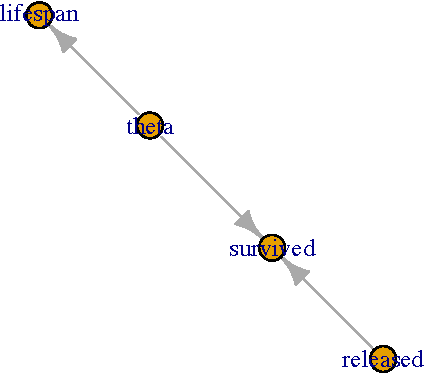
\includegraphics{banana-book_files/figure-latex/unnamed-chunk-67-1.pdf}

Second we compile the model with \texttt{compileNimble()}:

\begin{Shaded}
\begin{Highlighting}[]
\NormalTok{Csurvival }\OtherTok{\textless{}{-}} \FunctionTok{compileNimble}\NormalTok{(survival)}
\end{Highlighting}
\end{Shaded}

With \texttt{compileNimble()}, the C++ code is generated, compiled and loaded back into R so that it can be used in R (compiled model):

\begin{Shaded}
\begin{Highlighting}[]
\NormalTok{Csurvival}\SpecialCharTok{$}\NormalTok{theta}
\DocumentationTok{\#\# [1] 0.5}
\end{Highlighting}
\end{Shaded}

Now you have two versions of the model, \texttt{survival} is in R and \texttt{Csurvival} in C++. Being able to separate the steps of model building and parameter estimation is a strength of NIMBLE. This gives you a lot of flexibility at both steps. For example, imagine you would like to fit your model with maximum likelihood, then you can do it by wrapping your model in an R function that gets the likelihood and maximise this function. Using the C version of the model, you can write:

\begin{Shaded}
\begin{Highlighting}[]
\CommentTok{\# function for negative log{-}likelihood to minimize}
\NormalTok{f }\OtherTok{\textless{}{-}} \ControlFlowTok{function}\NormalTok{(par) \{}
\NormalTok{    Csurvival[[}\StringTok{\textquotesingle{}theta\textquotesingle{}}\NormalTok{]] }\OtherTok{\textless{}{-}}\NormalTok{ par }\CommentTok{\# assign par to theta }
\NormalTok{    ll }\OtherTok{\textless{}{-}}\NormalTok{ Csurvival}\SpecialCharTok{$}\FunctionTok{calculate}\NormalTok{() }\CommentTok{\# update log{-}likelihood with par value}
    \FunctionTok{return}\NormalTok{(}\SpecialCharTok{{-}}\NormalTok{ll) }\CommentTok{\# return negative log{-}likelihood}
\NormalTok{\}}
\CommentTok{\# evaluate function at 0.5 and 0.9}
\FunctionTok{f}\NormalTok{(}\FloatTok{0.5}\NormalTok{)}
\DocumentationTok{\#\# [1] 5.422}
\FunctionTok{f}\NormalTok{(}\FloatTok{0.9}\NormalTok{)}
\DocumentationTok{\#\# [1] 55.41}
\CommentTok{\# minimize function}
\NormalTok{out }\OtherTok{\textless{}{-}} \FunctionTok{optimize}\NormalTok{(f, }\AttributeTok{interval =} \FunctionTok{c}\NormalTok{(}\DecValTok{0}\NormalTok{,}\DecValTok{1}\NormalTok{))}
\FunctionTok{round}\NormalTok{(out}\SpecialCharTok{$}\NormalTok{minimum, }\DecValTok{2}\NormalTok{)}
\DocumentationTok{\#\# [1] 0.33}
\end{Highlighting}
\end{Shaded}

By maximising the likelihood (or minimising the negative log-likelihood), you obtain the maximum likelihood estimate of animal survival, which is exactly 19 surviving animals over 57 released animals or 0.33.

Third we create a MCMC configuration for our model with \texttt{configureMCMC()}:

\begin{Shaded}
\begin{Highlighting}[]
\NormalTok{survivalConf }\OtherTok{\textless{}{-}} \FunctionTok{configureMCMC}\NormalTok{(survival)}
\DocumentationTok{\#\# ===== Monitors =====}
\DocumentationTok{\#\# thin = 1: theta}
\DocumentationTok{\#\# ===== Samplers =====}
\DocumentationTok{\#\# RW sampler (1)}
\DocumentationTok{\#\#   {-} theta}
\end{Highlighting}
\end{Shaded}

This steps tells you the nodes that are monitored by default, and the MCMC samplers than have been assigned to them. Here \texttt{theta} is monitored, and samples from its posterior distribution are simulated with a random walk sampler similar to the Metropolis sampler we coded in the previous chapter in Section \ref{metropolis-algorithm}.

To monitor \texttt{lifespan} in addition to \texttt{theta}, you write:

\begin{Shaded}
\begin{Highlighting}[]
\NormalTok{survivalConf}\SpecialCharTok{$}\FunctionTok{addMonitors}\NormalTok{(}\FunctionTok{c}\NormalTok{(}\StringTok{"lifespan"}\NormalTok{))}
\DocumentationTok{\#\# thin = 1: theta, lifespan}
\NormalTok{survivalConf}
\DocumentationTok{\#\# ===== Monitors =====}
\DocumentationTok{\#\# thin = 1: theta, lifespan}
\DocumentationTok{\#\# ===== Samplers =====}
\DocumentationTok{\#\# RW sampler (1)}
\DocumentationTok{\#\#   {-} theta}
\end{Highlighting}
\end{Shaded}

Third, we create a MCMC function with \texttt{buildMCMC()} and compile it with \texttt{compileNimble()}:

\begin{Shaded}
\begin{Highlighting}[]
\NormalTok{survivalMCMC }\OtherTok{\textless{}{-}} \FunctionTok{buildMCMC}\NormalTok{(survivalConf)}
\NormalTok{CsurvivalMCMC }\OtherTok{\textless{}{-}} \FunctionTok{compileNimble}\NormalTok{(survivalMCMC, }\AttributeTok{project =}\NormalTok{ survival)}
\end{Highlighting}
\end{Shaded}

Note that models and \texttt{nimbleFunctions} need to be compiled before they can be used to specify a project.

Fourth, we run NIMBLE with \texttt{runMCMC()}:

\begin{Shaded}
\begin{Highlighting}[]
\NormalTok{n.iter }\OtherTok{\textless{}{-}} \DecValTok{5000}
\NormalTok{n.burnin }\OtherTok{\textless{}{-}} \DecValTok{1000}
\NormalTok{samples }\OtherTok{\textless{}{-}} \FunctionTok{runMCMC}\NormalTok{(}\AttributeTok{mcmc =}\NormalTok{ CsurvivalMCMC, }
                   \AttributeTok{niter =}\NormalTok{ n.iter,}
                   \AttributeTok{nburnin =}\NormalTok{ n.burnin)}
\DocumentationTok{\#\# |{-}{-}{-}{-}{-}{-}{-}{-}{-}{-}{-}{-}{-}|{-}{-}{-}{-}{-}{-}{-}{-}{-}{-}{-}{-}{-}|{-}{-}{-}{-}{-}{-}{-}{-}{-}{-}{-}{-}{-}|{-}{-}{-}{-}{-}{-}{-}{-}{-}{-}{-}{-}{-}|}
\DocumentationTok{\#\# |{-}{-}{-}{-}{-}{-}{-}{-}{-}{-}{-}{-}{-}{-}{-}{-}{-}{-}{-}{-}{-}{-}{-}{-}{-}{-}{-}{-}{-}{-}{-}{-}{-}{-}{-}{-}{-}{-}{-}{-}{-}{-}{-}{-}{-}{-}{-}{-}{-}{-}{-}{-}{-}{-}{-}|}
\end{Highlighting}
\end{Shaded}

We run a single chain but \texttt{runMCMC()} allows you to use multiple chains as with \texttt{nimbleMCMC()}.

You can look into \texttt{samples} which contains values simulated from the posterior distribution of the parameters we monitor:

\begin{Shaded}
\begin{Highlighting}[]
\FunctionTok{head}\NormalTok{(samples)}
\DocumentationTok{\#\#      lifespan  theta}
\DocumentationTok{\#\# [1,]   0.8572 0.3114}
\DocumentationTok{\#\# [2,]   0.8572 0.3114}
\DocumentationTok{\#\# [3,]   0.8572 0.3114}
\DocumentationTok{\#\# [4,]   0.8572 0.3114}
\DocumentationTok{\#\# [5,]   0.8572 0.3114}
\DocumentationTok{\#\# [6,]   0.8572 0.3114}
\end{Highlighting}
\end{Shaded}

From here, you can obtain numerical summaries with \texttt{samplesSummary()}:

\begin{Shaded}
\begin{Highlighting}[]
\FunctionTok{samplesSummary}\NormalTok{(samples)}
\DocumentationTok{\#\#            Mean Median St.Dev. 95\%CI\_low 95\%CI\_upp}
\DocumentationTok{\#\# lifespan 0.9336 0.9157 0.15679    0.6783    1.2884}
\DocumentationTok{\#\# theta    0.3380 0.3355 0.05949    0.2289    0.4602}
\end{Highlighting}
\end{Shaded}

At first glance, using several steps instead of doing all these at once with \texttt{nimbleMCMC()} seems odds. Why is it useful? Mastering the whole sequence of steps allows you to play around with samplers, by changing the samplers NIMBLE picks by default, or even writing your own samplers.

\hypertarget{playing-around-with-mcmc-samplers}{%
\section{Playing around with MCMC samplers}\label{playing-around-with-mcmc-samplers}}

\hypertarget{change-sampler}{%
\subsection{Changing default sampler}\label{change-sampler}}

What is the default sampler used by NIMBLE in our example? You can answer this question by inspecting the MCMC configuration obtained with \texttt{configureMCMC()}:

\begin{Shaded}
\begin{Highlighting}[]
\CommentTok{\#survivalConf \textless{}{-} configureMCMC(survival)}
\NormalTok{survivalConf}\SpecialCharTok{$}\FunctionTok{printSamplers}\NormalTok{()}
\DocumentationTok{\#\# [1] RW sampler: theta}
\end{Highlighting}
\end{Shaded}

Now that we have control on the MCMC configuration, let's mess it up. We start by removing the default sampler:

\begin{Shaded}
\begin{Highlighting}[]
\NormalTok{survivalConf}\SpecialCharTok{$}\FunctionTok{removeSamplers}\NormalTok{(}\FunctionTok{c}\NormalTok{(}\StringTok{\textquotesingle{}theta\textquotesingle{}}\NormalTok{))}
\NormalTok{survivalConf}\SpecialCharTok{$}\FunctionTok{printSamplers}\NormalTok{()}
\end{Highlighting}
\end{Shaded}

And we change it for a slice sampler:

\begin{Shaded}
\begin{Highlighting}[]
\NormalTok{survivalConf}\SpecialCharTok{$}\FunctionTok{addSampler}\NormalTok{(}\AttributeTok{target =} \FunctionTok{c}\NormalTok{(}\StringTok{\textquotesingle{}theta\textquotesingle{}}\NormalTok{),}
                        \AttributeTok{type =} \StringTok{\textquotesingle{}slice\textquotesingle{}}\NormalTok{)}
\NormalTok{survivalConf}\SpecialCharTok{$}\FunctionTok{printSamplers}\NormalTok{()}
\DocumentationTok{\#\# [1] slice sampler: theta}
\end{Highlighting}
\end{Shaded}

Now you can resume the workflow:

\begin{Shaded}
\begin{Highlighting}[]
\CommentTok{\# create a new MCMC function and compile it:}
\NormalTok{survivalMCMC2 }\OtherTok{\textless{}{-}} \FunctionTok{buildMCMC}\NormalTok{(survivalConf)}
\NormalTok{CsurvivalMCMC2 }\OtherTok{\textless{}{-}} \FunctionTok{compileNimble}\NormalTok{(survivalMCMC2, }
                                \AttributeTok{project =}\NormalTok{ survival,}
                                \AttributeTok{resetFunctions =} \ConstantTok{TRUE}\NormalTok{) }\CommentTok{\# to compile new functions }
                                                       \CommentTok{\# into existing project, }
                                                       \CommentTok{\# need to reset nimbleFunctions}
\CommentTok{\# run NIMBLE:}
\NormalTok{samples2 }\OtherTok{\textless{}{-}} \FunctionTok{runMCMC}\NormalTok{(}\AttributeTok{mcmc =}\NormalTok{ CsurvivalMCMC2, }
                    \AttributeTok{niter =}\NormalTok{ n.iter,}
                    \AttributeTok{nburnin =}\NormalTok{ n.burnin)}
\DocumentationTok{\#\# |{-}{-}{-}{-}{-}{-}{-}{-}{-}{-}{-}{-}{-}|{-}{-}{-}{-}{-}{-}{-}{-}{-}{-}{-}{-}{-}|{-}{-}{-}{-}{-}{-}{-}{-}{-}{-}{-}{-}{-}|{-}{-}{-}{-}{-}{-}{-}{-}{-}{-}{-}{-}{-}|}
\DocumentationTok{\#\# |{-}{-}{-}{-}{-}{-}{-}{-}{-}{-}{-}{-}{-}{-}{-}{-}{-}{-}{-}{-}{-}{-}{-}{-}{-}{-}{-}{-}{-}{-}{-}{-}{-}{-}{-}{-}{-}{-}{-}{-}{-}{-}{-}{-}{-}{-}{-}{-}{-}{-}{-}{-}{-}{-}{-}|}
\CommentTok{\# obtain numerical summaries:}
\FunctionTok{samplesSummary}\NormalTok{(samples2)}
\DocumentationTok{\#\#            Mean Median St.Dev. 95\%CI\_low 95\%CI\_upp}
\DocumentationTok{\#\# lifespan 0.9385 0.9204 0.16297    0.6681    1.3004}
\DocumentationTok{\#\# theta    0.3396 0.3374 0.06151    0.2238    0.4635}
\end{Highlighting}
\end{Shaded}

NIMBLE implements many samplers, and a list is available with \texttt{?samplers}. For example, high correlation in (regression) parameters can make independent samplers inefficient. In that situation, block sampling might help which consists in proposing candidate values from a multivariate distribution that acknowledges correlation between parameters. \textbf{Say something on how default samplers are chosen by NIMBLE?}

\hypertarget{coding-your-own-sampler}{%
\subsection{Coding your own sampler}\label{coding-your-own-sampler}}

Allowing you to code your own sampler is another topic on which NIMBLE thrives. As an example, we focus on the Metropolis algorithm of Section \ref{metropolis-algorithm} which we coded in R. In this section, we make it a \texttt{nimbleFunction} so that we can use it within our model:

\begin{Shaded}
\begin{Highlighting}[]
\NormalTok{my\_metropolis }\OtherTok{\textless{}{-}} \FunctionTok{nimbleFunction}\NormalTok{(}
  \AttributeTok{name =} \StringTok{\textquotesingle{}my\_metropolis\textquotesingle{}}\NormalTok{, }\CommentTok{\# fancy name for our MCMC sampler}
  \AttributeTok{contains =}\NormalTok{ sampler\_BASE,}
  \AttributeTok{setup =} \ControlFlowTok{function}\NormalTok{(model, mvSaved, target, control) \{}
    \CommentTok{\# i) get dependencies for \textquotesingle{}target\textquotesingle{} in \textquotesingle{}model\textquotesingle{}}
\NormalTok{    calcNodes }\OtherTok{\textless{}{-}}\NormalTok{ model}\SpecialCharTok{$}\FunctionTok{getDependencies}\NormalTok{(target) }
    \CommentTok{\# ii) get sd of proposal distribution}
\NormalTok{    scale }\OtherTok{\textless{}{-}}\NormalTok{ control}\SpecialCharTok{$}\NormalTok{scale }
\NormalTok{  \},}
  \AttributeTok{run =} \ControlFlowTok{function}\NormalTok{() \{}
    \CommentTok{\# (1) log{-}lik at current value}
\NormalTok{    initialLP }\OtherTok{\textless{}{-}}\NormalTok{ model}\SpecialCharTok{$}\FunctionTok{getLogProb}\NormalTok{(calcNodes) }
    \CommentTok{\# (2) current parameter value}
\NormalTok{    current }\OtherTok{\textless{}{-}}\NormalTok{ model[[target]] }
    \CommentTok{\# (3) logit transform}
\NormalTok{    lcurrent }\OtherTok{\textless{}{-}} \FunctionTok{log}\NormalTok{(current }\SpecialCharTok{/}\NormalTok{ (}\DecValTok{1} \SpecialCharTok{{-}}\NormalTok{ current))}
    \CommentTok{\# (4) propose candidate value}
\NormalTok{    lproposal }\OtherTok{\textless{}{-}}\NormalTok{ lcurrent  }\SpecialCharTok{+} \FunctionTok{rnorm}\NormalTok{(}\DecValTok{1}\NormalTok{, }\AttributeTok{mean =} \DecValTok{0}\NormalTok{, scale) }
    \CommentTok{\# (5) back{-}transform}
\NormalTok{    proposal }\OtherTok{\textless{}{-}} \FunctionTok{plogis}\NormalTok{(lproposal)}
    \CommentTok{\# (6) plug candidate value in model }
\NormalTok{    model[[target]] }\OtherTok{\textless{}\textless{}{-}}\NormalTok{ proposal }
    \CommentTok{\# (7) log{-}lik at candidate value}
\NormalTok{    proposalLP }\OtherTok{\textless{}{-}}\NormalTok{ model}\SpecialCharTok{$}\FunctionTok{calculate}\NormalTok{(calcNodes)}
    \CommentTok{\# (8) compute lik ratio on log scale}
\NormalTok{    lMHR }\OtherTok{\textless{}{-}}\NormalTok{ proposalLP }\SpecialCharTok{{-}}\NormalTok{ initialLP }
    \CommentTok{\# (9) spin continuous spinner and compare to ratio}
    \ControlFlowTok{if}\NormalTok{(}\FunctionTok{runif}\NormalTok{(}\DecValTok{1}\NormalTok{,}\DecValTok{0}\NormalTok{,}\DecValTok{1}\NormalTok{) }\SpecialCharTok{\textless{}} \FunctionTok{exp}\NormalTok{(lMHR)) \{ }
      \CommentTok{\# (10) if candidate value is accepted, update current value}
      \FunctionTok{copy}\NormalTok{(}\AttributeTok{from =}\NormalTok{ model, }\AttributeTok{to =}\NormalTok{ mvSaved, }\AttributeTok{nodes =}\NormalTok{ calcNodes, }\AttributeTok{logProb =} \ConstantTok{TRUE}\NormalTok{, }\AttributeTok{row =} \DecValTok{1}\NormalTok{)}
\NormalTok{    \} }\ControlFlowTok{else}\NormalTok{ \{}
      \DocumentationTok{\#\# (11) if candidate value is accepted, keep current value}
      \FunctionTok{copy}\NormalTok{(}\AttributeTok{from =}\NormalTok{ mvSaved, }\AttributeTok{to =}\NormalTok{ model, }\AttributeTok{nodes =}\NormalTok{ calcNodes, }\AttributeTok{logProb =} \ConstantTok{TRUE}\NormalTok{, }\AttributeTok{row =} \DecValTok{1}\NormalTok{)}
\NormalTok{    \}}
\NormalTok{  \},}
  \AttributeTok{methods =} \FunctionTok{list}\NormalTok{(}
    \AttributeTok{reset =} \ControlFlowTok{function}\NormalTok{() \{\}}
\NormalTok{  )}
\NormalTok{)}
\end{Highlighting}
\end{Shaded}

Compared to \texttt{nimbleFunctions} we wrote earlier, \texttt{my\_metropolis()} contains a \texttt{setup} function which i) gets the dependencies of the parameter to update in the \texttt{run} function with Metropolis, the target node, that would be \texttt{theta} in our example and ii) extracts control parameters, that would be \texttt{scale} the standard deviation of the proposal distribution in our example. Then the \texttt{run} function implements the steps of the Metropolis algorithm: (1) get the log-likelihood function evaluated at the current value, (2) get the current value, (3) apply the logit transform to it, (4) propose a candidate value by perturbing the current value with some normal noise controled by the standard deviation \texttt{scale}, (5) back-transform the candidate value and (6) plug it in the model, (7) calculate the log-likelihood function at the candidate value, (8) compute the Metropolis ratio on the log scale, (9) compare output of a spinner and the Metropolis ratio to decide whether to (10) accept the candidate value and copy from the model to \texttt{mvSaved} or (11) reject it and keep the current value by copying from \texttt{mvSaved} to the model. Because this \texttt{nimbleFunction} is to be used as a MCMC sampler, several constraints need to be respected like having a \texttt{contains\ =\ sampler\_BASE} statement or using the four arguments \texttt{model}, \texttt{mvSaved}, \texttt{target} and \texttt{control} in the \texttt{setup} function. Of course, NIMBLE implements a more advanced and efficient version of the Metropolis algorithm, you can look into it at \url{https://github.com/cran/nimble/blob/master/R/MCMC_samplers.R\#L184}.

Now that we have our user-defined MCMC algorithm, we can change the default sampler for our new sampler as in Section \ref{change-sampler}. We start from scratch:

\begin{Shaded}
\begin{Highlighting}[]
\NormalTok{model }\OtherTok{\textless{}{-}} \FunctionTok{nimbleCode}\NormalTok{(\{}
  \CommentTok{\# likelihood}
\NormalTok{  survived }\SpecialCharTok{\textasciitilde{}} \FunctionTok{dbinom}\NormalTok{(theta, released)}
  \CommentTok{\# prior}
\NormalTok{  theta }\SpecialCharTok{\textasciitilde{}} \FunctionTok{dunif}\NormalTok{(}\DecValTok{0}\NormalTok{, }\DecValTok{1}\NormalTok{)}
\NormalTok{\})}
\NormalTok{my.data }\OtherTok{\textless{}{-}} \FunctionTok{list}\NormalTok{(}\AttributeTok{survived =} \DecValTok{19}\NormalTok{, }\AttributeTok{released =} \DecValTok{57}\NormalTok{)}
\NormalTok{initial.values }\OtherTok{\textless{}{-}} \ControlFlowTok{function}\NormalTok{() }\FunctionTok{list}\NormalTok{(}\AttributeTok{theta =} \FunctionTok{runif}\NormalTok{(}\DecValTok{1}\NormalTok{,}\DecValTok{0}\NormalTok{,}\DecValTok{1}\NormalTok{))}
\NormalTok{survival }\OtherTok{\textless{}{-}} \FunctionTok{nimbleModel}\NormalTok{(}\AttributeTok{code =}\NormalTok{ model, }
                        \AttributeTok{data =}\NormalTok{ my.data, }
                        \AttributeTok{inits =} \FunctionTok{initial.values}\NormalTok{())}
\NormalTok{Csurvival }\OtherTok{\textless{}{-}} \FunctionTok{compileNimble}\NormalTok{(survival)}
\NormalTok{survivalConf }\OtherTok{\textless{}{-}} \FunctionTok{configureMCMC}\NormalTok{(survival)}
\DocumentationTok{\#\# ===== Monitors =====}
\DocumentationTok{\#\# thin = 1: theta}
\DocumentationTok{\#\# ===== Samplers =====}
\DocumentationTok{\#\# RW sampler (1)}
\DocumentationTok{\#\#   {-} theta}
\end{Highlighting}
\end{Shaded}

We print the samplers used by default, remove the default sampler for \texttt{theta}, replace it with our \texttt{my\_metropolis()} sampler with the standard deviation of the proposal distribution set to 0.1, and print again to make sure NIMBLE now uses our new sampler:

\begin{Shaded}
\begin{Highlighting}[]
\NormalTok{survivalConf}\SpecialCharTok{$}\FunctionTok{printSamplers}\NormalTok{()}
\DocumentationTok{\#\# [1] RW sampler: theta}
\NormalTok{survivalConf}\SpecialCharTok{$}\FunctionTok{removeSamplers}\NormalTok{(}\FunctionTok{c}\NormalTok{(}\StringTok{\textquotesingle{}theta\textquotesingle{}}\NormalTok{))}
\NormalTok{survivalConf}\SpecialCharTok{$}\FunctionTok{addSampler}\NormalTok{(}\AttributeTok{target =} \StringTok{\textquotesingle{}theta\textquotesingle{}}\NormalTok{, }
                        \AttributeTok{type =} \StringTok{\textquotesingle{}my\_metropolis\textquotesingle{}}\NormalTok{, }
                        \AttributeTok{control =} \FunctionTok{list}\NormalTok{(}\AttributeTok{scale =} \FloatTok{0.1}\NormalTok{)) }\CommentTok{\# standard deviation}
                                                     \CommentTok{\# of proposal distribution}
\NormalTok{survivalConf}\SpecialCharTok{$}\FunctionTok{printSamplers}\NormalTok{()}
\DocumentationTok{\#\# [1] my\_metropolis sampler: theta,  scale: 0.10000000000000001}
\end{Highlighting}
\end{Shaded}

The rest of the workflow is unchanged:

\begin{Shaded}
\begin{Highlighting}[]
\NormalTok{survivalMCMC }\OtherTok{\textless{}{-}} \FunctionTok{buildMCMC}\NormalTok{(survivalConf)}
\NormalTok{CsurvivalMCMC }\OtherTok{\textless{}{-}} \FunctionTok{compileNimble}\NormalTok{(survivalMCMC, }
                               \AttributeTok{project =}\NormalTok{ survival)}
\NormalTok{samples }\OtherTok{\textless{}{-}} \FunctionTok{runMCMC}\NormalTok{(}\AttributeTok{mcmc =}\NormalTok{ CsurvivalMCMC, }
                   \AttributeTok{niter =} \DecValTok{5000}\NormalTok{, }
                   \AttributeTok{nburnin =} \DecValTok{1000}\NormalTok{)}
\DocumentationTok{\#\# |{-}{-}{-}{-}{-}{-}{-}{-}{-}{-}{-}{-}{-}|{-}{-}{-}{-}{-}{-}{-}{-}{-}{-}{-}{-}{-}|{-}{-}{-}{-}{-}{-}{-}{-}{-}{-}{-}{-}{-}|{-}{-}{-}{-}{-}{-}{-}{-}{-}{-}{-}{-}{-}|}
\DocumentationTok{\#\# |{-}{-}{-}{-}{-}{-}{-}{-}{-}{-}{-}{-}{-}{-}{-}{-}{-}{-}{-}{-}{-}{-}{-}{-}{-}{-}{-}{-}{-}{-}{-}{-}{-}{-}{-}{-}{-}{-}{-}{-}{-}{-}{-}{-}{-}{-}{-}{-}{-}{-}{-}{-}{-}{-}{-}|}
\FunctionTok{samplesSummary}\NormalTok{(samples)}
\DocumentationTok{\#\#         Mean Median St.Dev. 95\%CI\_low 95\%CI\_upp}
\DocumentationTok{\#\# theta 0.3335 0.3311 0.06665    0.2128    0.4652}
\end{Highlighting}
\end{Shaded}

You can re-run the analysis by setting the standard deviation of the proposal to different values, say 1 and 10, and compare Figure \ref{fig:traceown} to traceplots we obtained with our R implementation of the Metropolis algorithm in the previous chapter at Figure \ref{fig:tracechainlength}:

\begin{figure}

{\centering 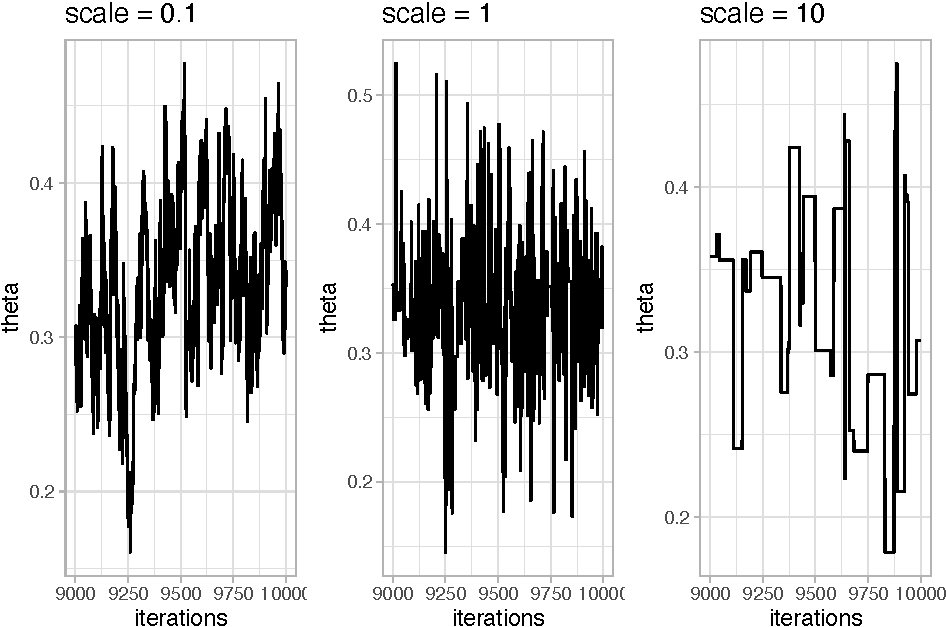
\includegraphics[width=1\linewidth]{banana-book_files/figure-latex/traceown-1} 

}

\caption{Trace plots for different values of the standard deviation (scale) of the proposal distribution.}\label{fig:traceown}
\end{figure}

\hypertarget{tips-and-tricks}{%
\section{Tips and tricks}\label{tips-and-tricks}}

Before closing this chapter on NIMBLE, I thought it'd be useful to have a section gathering a few tips and tricks that would make your life easier. \textbf{These are my tips and tricks, NIMBLE users, I'd be happy to hear yours: \href{mailto:olivier.gimenez@cefe.cnrs.fr}{email me}, \href{https://github.com/oliviergimenez/banana-book/edit/master/nimble.Rmd}{edit the chapter} or \href{https://github.com/oliviergimenez/banana-book/issues}{file an issue} on GitHub.}

\hypertarget{flexible-specification-of-distributions}{%
\subsection{Flexible specification of distributions}\label{flexible-specification-of-distributions}}

In other sotware like JAGS, the normal distribution is parameterized with mean \texttt{mu} and a parameter called precision, often denoted \texttt{tau}, the inverse of the variance you are used to. Say we use a normal prior on some parameter \texttt{epsilon} with \texttt{epsilon\ \textasciitilde{}\ dnorm(mu,\ tau)}. We'd like this prior to be vague, therefore \texttt{tau} should be small, say 0.01 so that the variance of the normal distribution is large, 1/0.01 = 100 here. This subtlety is the source of problems (and frustration) when you forget that the second parameter is precision and use \texttt{epsilon\ \textasciitilde{}\ dnorm(mu,\ 100)}, because then the variance is actually 1/100 = 0.01 and the prior is very informative, and peaked on \texttt{mu}. In NIMBLE you can use this parameterisation as well as the more natural parameterisation \texttt{epsilon\ \textasciitilde{}\ dnorm(mu,\ sd\ =\ 100)}.

\hypertarget{the-end-of-empty-indices}{%
\subsection{The end of empty indices}\label{the-end-of-empty-indices}}

NIMBLE does not guess the dimensions of objects. In other software like JAGS you can write \texttt{sum.x\ \textless{}-\ sum(x{[}{]})} to calculate the sum over all components of \texttt{x}. In NIMBLE you need to write \texttt{sum.x\ \textless{}-\ sum(x{[}1:n{]})} the sum the components of \texttt{x} from 1 up to n.~Specifying dimensions can be annoying, but it forces me to think of what I am doing and keep my code self-explaining.

\hypertarget{faster-compilation}{%
\subsection{Faster compilation}\label{faster-compilation}}

You might have noticed that compilation in NIMBLE takes time. When you have large models (with lots of nodes), compilation can take forever. You can set \texttt{calculate\ =\ FALSE} in \texttt{nimbleModel()} to disable the calculation of all deterministic nodes and log-likelihood. You can also use \texttt{useConjugacy\ =\ FALSE} in \texttt{configureMCMC()} to disable the search for conjugate samplers. With the animal survival example, you would do:

\begin{Shaded}
\begin{Highlighting}[]
\NormalTok{model }\OtherTok{\textless{}{-}} \FunctionTok{nimbleCode}\NormalTok{(\{}
  \CommentTok{\# likelihood}
\NormalTok{  survived }\SpecialCharTok{\textasciitilde{}} \FunctionTok{dbinom}\NormalTok{(theta, released)}
  \CommentTok{\# prior}
\NormalTok{  theta }\SpecialCharTok{\textasciitilde{}} \FunctionTok{dunif}\NormalTok{(}\DecValTok{0}\NormalTok{, }\DecValTok{1}\NormalTok{)}
\NormalTok{\})}
\NormalTok{my.data }\OtherTok{\textless{}{-}} \FunctionTok{list}\NormalTok{(}\AttributeTok{survived =} \DecValTok{19}\NormalTok{, }\AttributeTok{released =} \DecValTok{57}\NormalTok{)}
\NormalTok{initial.values }\OtherTok{\textless{}{-}} \ControlFlowTok{function}\NormalTok{() }\FunctionTok{list}\NormalTok{(}\AttributeTok{theta =} \FunctionTok{runif}\NormalTok{(}\DecValTok{1}\NormalTok{,}\DecValTok{0}\NormalTok{,}\DecValTok{1}\NormalTok{))}
\NormalTok{survival }\OtherTok{\textless{}{-}} \FunctionTok{nimbleModel}\NormalTok{(}\AttributeTok{code =}\NormalTok{ model, }
                        \AttributeTok{data =}\NormalTok{ my.data, }
                        \AttributeTok{inits =} \FunctionTok{initial.values}\NormalTok{(),}
                        \AttributeTok{calculate =} \ConstantTok{FALSE}\NormalTok{) }\CommentTok{\# first tip}
\NormalTok{Csurvival }\OtherTok{\textless{}{-}} \FunctionTok{compileNimble}\NormalTok{(survival)}
\NormalTok{survivalConf }\OtherTok{\textless{}{-}} \FunctionTok{configureMCMC}\NormalTok{(survival)}
\DocumentationTok{\#\# ===== Monitors =====}
\DocumentationTok{\#\# thin = 1: theta}
\DocumentationTok{\#\# ===== Samplers =====}
\DocumentationTok{\#\# RW sampler (1)}
\DocumentationTok{\#\#   {-} theta}
\NormalTok{survivalMCMC }\OtherTok{\textless{}{-}} \FunctionTok{buildMCMC}\NormalTok{(survivalConf, }\AttributeTok{useConjugacy =} \ConstantTok{FALSE}\NormalTok{) }\CommentTok{\# second tip}
\NormalTok{CsurvivalMCMC }\OtherTok{\textless{}{-}} \FunctionTok{compileNimble}\NormalTok{(survivalMCMC, }
                               \AttributeTok{project =}\NormalTok{ survival)}
\NormalTok{samples }\OtherTok{\textless{}{-}} \FunctionTok{runMCMC}\NormalTok{(}\AttributeTok{mcmc =}\NormalTok{ CsurvivalMCMC, }
                   \AttributeTok{niter =} \DecValTok{5000}\NormalTok{, }
                   \AttributeTok{nburnin =} \DecValTok{1000}\NormalTok{)}
\DocumentationTok{\#\# |{-}{-}{-}{-}{-}{-}{-}{-}{-}{-}{-}{-}{-}|{-}{-}{-}{-}{-}{-}{-}{-}{-}{-}{-}{-}{-}|{-}{-}{-}{-}{-}{-}{-}{-}{-}{-}{-}{-}{-}|{-}{-}{-}{-}{-}{-}{-}{-}{-}{-}{-}{-}{-}|}
\DocumentationTok{\#\# |{-}{-}{-}{-}{-}{-}{-}{-}{-}{-}{-}{-}{-}{-}{-}{-}{-}{-}{-}{-}{-}{-}{-}{-}{-}{-}{-}{-}{-}{-}{-}{-}{-}{-}{-}{-}{-}{-}{-}{-}{-}{-}{-}{-}{-}{-}{-}{-}{-}{-}{-}{-}{-}{-}{-}|}
\FunctionTok{samplesSummary}\NormalTok{(samples)}
\DocumentationTok{\#\#         Mean Median St.Dev. 95\%CI\_low 95\%CI\_upp}
\DocumentationTok{\#\# theta 0.3398 0.3379 0.06188     0.225    0.4687}
\end{Highlighting}
\end{Shaded}

\hypertarget{running-nimble-a-little-bit-longer}{%
\subsection{Running NIMBLE a little bit longer}\label{running-nimble-a-little-bit-longer}}

Sometimes it is useful to run your MCMC chains a little bit longer to improve convergence. Re-starting from the run in previous section, you can use:

\begin{Shaded}
\begin{Highlighting}[]
\NormalTok{niter\_ad }\OtherTok{\textless{}{-}} \DecValTok{6000}
\NormalTok{CsurvivalMCMC}\SpecialCharTok{$}\FunctionTok{run}\NormalTok{(niter\_ad, }\AttributeTok{reset =} \ConstantTok{FALSE}\NormalTok{)}
\DocumentationTok{\#\# |{-}{-}{-}{-}{-}{-}{-}{-}{-}{-}{-}{-}{-}|{-}{-}{-}{-}{-}{-}{-}{-}{-}{-}{-}{-}{-}|{-}{-}{-}{-}{-}{-}{-}{-}{-}{-}{-}{-}{-}|{-}{-}{-}{-}{-}{-}{-}{-}{-}{-}{-}{-}{-}|}
\DocumentationTok{\#\# |{-}{-}{-}{-}{-}{-}{-}{-}{-}{-}{-}{-}{-}{-}{-}{-}{-}{-}{-}{-}{-}{-}{-}{-}{-}{-}{-}{-}{-}{-}{-}{-}{-}{-}{-}{-}{-}{-}{-}{-}{-}{-}{-}{-}{-}{-}{-}{-}{-}{-}{-}{-}{-}{-}{-}|}
\DocumentationTok{\#\# NULL}
\end{Highlighting}
\end{Shaded}

Then you can extract the matrix of previous MCMC samples augmented with new ones and obtain numerical summaries:

\begin{Shaded}
\begin{Highlighting}[]
\NormalTok{more\_samples }\OtherTok{\textless{}{-}} \FunctionTok{as.matrix}\NormalTok{(CsurvivalMCMC}\SpecialCharTok{$}\NormalTok{mvSamples)}
\FunctionTok{samplesSummary}\NormalTok{(more\_samples)}
\DocumentationTok{\#\#         Mean Median St.Dev. 95\%CI\_low 95\%CI\_upp}
\DocumentationTok{\#\# theta 0.3398 0.3381 0.06138     0.225    0.4622}
\end{Highlighting}
\end{Shaded}

You can check that \texttt{more\_samples} contains 10000 samples, 4000 from the call to \texttt{runMCMC()} plus 6000 additional samples.

\hypertarget{reproducibility}{%
\subsection{Reproducibility}\label{reproducibility}}

If you want your results to be reproducible, you can control the state of R the random number generator with the \texttt{setSeed} argument in function \texttt{nimbleMCMC()} and \texttt{runMCMC()}. Going back to the animal survival example, you can check that two calls to \texttt{nimbleMCMC()} give the same results when \texttt{setSeed} is set to the same value:

\begin{Shaded}
\begin{Highlighting}[]
\CommentTok{\# first call to nimbleMCMC()}
\NormalTok{mcmc.output1 }\OtherTok{\textless{}{-}} \FunctionTok{nimbleMCMC}\NormalTok{(}\AttributeTok{code =}\NormalTok{ model,}
                          \AttributeTok{data =}\NormalTok{ my.data,}
                          \AttributeTok{inits =}\NormalTok{ initial.values,}
                          \AttributeTok{niter =} \DecValTok{5000}\NormalTok{,}
                          \AttributeTok{nburnin =} \DecValTok{1000}\NormalTok{,}
                          \AttributeTok{nchains =} \DecValTok{3}\NormalTok{,}
                          \AttributeTok{summary =} \ConstantTok{TRUE}\NormalTok{,}
                          \AttributeTok{setSeed =} \DecValTok{123}\NormalTok{)}
\DocumentationTok{\#\# |{-}{-}{-}{-}{-}{-}{-}{-}{-}{-}{-}{-}{-}|{-}{-}{-}{-}{-}{-}{-}{-}{-}{-}{-}{-}{-}|{-}{-}{-}{-}{-}{-}{-}{-}{-}{-}{-}{-}{-}|{-}{-}{-}{-}{-}{-}{-}{-}{-}{-}{-}{-}{-}|}
\DocumentationTok{\#\# |{-}{-}{-}{-}{-}{-}{-}{-}{-}{-}{-}{-}{-}{-}{-}{-}{-}{-}{-}{-}{-}{-}{-}{-}{-}{-}{-}{-}{-}{-}{-}{-}{-}{-}{-}{-}{-}{-}{-}{-}{-}{-}{-}{-}{-}{-}{-}{-}{-}{-}{-}{-}{-}{-}{-}|}
\DocumentationTok{\#\# |{-}{-}{-}{-}{-}{-}{-}{-}{-}{-}{-}{-}{-}|{-}{-}{-}{-}{-}{-}{-}{-}{-}{-}{-}{-}{-}|{-}{-}{-}{-}{-}{-}{-}{-}{-}{-}{-}{-}{-}|{-}{-}{-}{-}{-}{-}{-}{-}{-}{-}{-}{-}{-}|}
\DocumentationTok{\#\# |{-}{-}{-}{-}{-}{-}{-}{-}{-}{-}{-}{-}{-}{-}{-}{-}{-}{-}{-}{-}{-}{-}{-}{-}{-}{-}{-}{-}{-}{-}{-}{-}{-}{-}{-}{-}{-}{-}{-}{-}{-}{-}{-}{-}{-}{-}{-}{-}{-}{-}{-}{-}{-}{-}{-}|}
\DocumentationTok{\#\# |{-}{-}{-}{-}{-}{-}{-}{-}{-}{-}{-}{-}{-}|{-}{-}{-}{-}{-}{-}{-}{-}{-}{-}{-}{-}{-}|{-}{-}{-}{-}{-}{-}{-}{-}{-}{-}{-}{-}{-}|{-}{-}{-}{-}{-}{-}{-}{-}{-}{-}{-}{-}{-}|}
\DocumentationTok{\#\# |{-}{-}{-}{-}{-}{-}{-}{-}{-}{-}{-}{-}{-}{-}{-}{-}{-}{-}{-}{-}{-}{-}{-}{-}{-}{-}{-}{-}{-}{-}{-}{-}{-}{-}{-}{-}{-}{-}{-}{-}{-}{-}{-}{-}{-}{-}{-}{-}{-}{-}{-}{-}{-}{-}{-}|}
\CommentTok{\# second call to nimbleMCMC()}
\NormalTok{mcmc.output2 }\OtherTok{\textless{}{-}} \FunctionTok{nimbleMCMC}\NormalTok{(}\AttributeTok{code =}\NormalTok{ model,}
                          \AttributeTok{data =}\NormalTok{ my.data,}
                          \AttributeTok{inits =}\NormalTok{ initial.values,}
                          \AttributeTok{niter =} \DecValTok{5000}\NormalTok{,}
                          \AttributeTok{nburnin =} \DecValTok{1000}\NormalTok{,}
                          \AttributeTok{nchains =} \DecValTok{3}\NormalTok{,}
                          \AttributeTok{summary =} \ConstantTok{TRUE}\NormalTok{,}
                          \AttributeTok{setSeed =} \DecValTok{123}\NormalTok{)}
\DocumentationTok{\#\# |{-}{-}{-}{-}{-}{-}{-}{-}{-}{-}{-}{-}{-}|{-}{-}{-}{-}{-}{-}{-}{-}{-}{-}{-}{-}{-}|{-}{-}{-}{-}{-}{-}{-}{-}{-}{-}{-}{-}{-}|{-}{-}{-}{-}{-}{-}{-}{-}{-}{-}{-}{-}{-}|}
\DocumentationTok{\#\# |{-}{-}{-}{-}{-}{-}{-}{-}{-}{-}{-}{-}{-}{-}{-}{-}{-}{-}{-}{-}{-}{-}{-}{-}{-}{-}{-}{-}{-}{-}{-}{-}{-}{-}{-}{-}{-}{-}{-}{-}{-}{-}{-}{-}{-}{-}{-}{-}{-}{-}{-}{-}{-}{-}{-}|}
\DocumentationTok{\#\# |{-}{-}{-}{-}{-}{-}{-}{-}{-}{-}{-}{-}{-}|{-}{-}{-}{-}{-}{-}{-}{-}{-}{-}{-}{-}{-}|{-}{-}{-}{-}{-}{-}{-}{-}{-}{-}{-}{-}{-}|{-}{-}{-}{-}{-}{-}{-}{-}{-}{-}{-}{-}{-}|}
\DocumentationTok{\#\# |{-}{-}{-}{-}{-}{-}{-}{-}{-}{-}{-}{-}{-}{-}{-}{-}{-}{-}{-}{-}{-}{-}{-}{-}{-}{-}{-}{-}{-}{-}{-}{-}{-}{-}{-}{-}{-}{-}{-}{-}{-}{-}{-}{-}{-}{-}{-}{-}{-}{-}{-}{-}{-}{-}{-}|}
\DocumentationTok{\#\# |{-}{-}{-}{-}{-}{-}{-}{-}{-}{-}{-}{-}{-}|{-}{-}{-}{-}{-}{-}{-}{-}{-}{-}{-}{-}{-}|{-}{-}{-}{-}{-}{-}{-}{-}{-}{-}{-}{-}{-}|{-}{-}{-}{-}{-}{-}{-}{-}{-}{-}{-}{-}{-}|}
\DocumentationTok{\#\# |{-}{-}{-}{-}{-}{-}{-}{-}{-}{-}{-}{-}{-}{-}{-}{-}{-}{-}{-}{-}{-}{-}{-}{-}{-}{-}{-}{-}{-}{-}{-}{-}{-}{-}{-}{-}{-}{-}{-}{-}{-}{-}{-}{-}{-}{-}{-}{-}{-}{-}{-}{-}{-}{-}{-}|}
\CommentTok{\# outputs from both calls are the same}
\NormalTok{mcmc.output1}\SpecialCharTok{$}\NormalTok{summary}\SpecialCharTok{$}\NormalTok{all.chains}
\DocumentationTok{\#\#         Mean Median St.Dev. 95\%CI\_low 95\%CI\_upp}
\DocumentationTok{\#\# theta 0.3387  0.336 0.05968    0.2282    0.4608}
\NormalTok{mcmc.output2}\SpecialCharTok{$}\NormalTok{summary}\SpecialCharTok{$}\NormalTok{all.chains}
\DocumentationTok{\#\#         Mean Median St.Dev. 95\%CI\_low 95\%CI\_upp}
\DocumentationTok{\#\# theta 0.3387  0.336 0.05968    0.2282    0.4608}
\end{Highlighting}
\end{Shaded}

\hypertarget{thoughts}{%
\section{Thoughts}\label{thoughts}}

\begin{itemize}
\tightlist
\item
  Something on parallelization à la jagsUI? \url{https://r-nimble.org/nimbleExamples/parallelizing_NIMBLE.html}
\end{itemize}

\begin{itemize}
\tightlist
\item
  Something on initialization and the NA (or NaN) messages.
\end{itemize}

\begin{itemize}
\item
  Something on vectorization?
\item
  Something on how to use NIMBLE to simulate data? Example with generate initial values for complex models? \url{https://r-nimble.org/nimbleExamples/simulation_from_model.html}. Then pbs with initial values.
\item
  Why NIMBLE over Stan? i) The BUGS language is cool, ii) discrete latent states easier to deal with NIMBLE, no need to marginalise like with Stan (ref forward to relevant section of the book for marginalization in NIMBLE), iii) also HMC is on its way in NIMBLE, so NIMBLE includes STAN and has so much more to offer the users.
\item
  Introduce MCMC efficiency?
\end{itemize}

\hypertarget{summary-1}{%
\section{Summary}\label{summary-1}}

\begin{itemize}
\item
  NIMBLE is an R package that implements for you MCMC algorithms to generate samples from the posterior distribution of model parameters. You only have to specify a likelihood and priors using the BUGS language to apply the Bayes theorem.
\item
  NIMBLE is more than just another MCMC engine. It provides a programming environment so that you have full control when building models and estimating parameters.
\item
  At the core of NIMBLE are \texttt{nimbleFunctions} which you can write and compile for faster computation. With \texttt{nimbleFunctions} you can mimic basic R syntax, work with vectors and matrices, use logical operators and flow control, and specify many distributions.
\item
  There are two workflows to run NIMBLE. In most situations, \texttt{nimbleMCMC()} will serve you well. When you need more control, you can adopt a detailed workflow with \texttt{nimbleModel()}, \texttt{configureMCMC()}, \texttt{buildMCMC()}, \texttt{compileNimble()} and \texttt{runMCMC()}.
\item
  By having full control of the workflow, you can change default MCMC samplers and even write your own samplers.
\end{itemize}

\hypertarget{suggested-reading-1}{%
\section{Suggested reading}\label{suggested-reading-1}}

In this chapter, I have only scratched the surface of what NIMBLE is capable of. Below is a list of pointers that should help you going further with NIMBLE.

\begin{itemize}
\item
  The NIMBLE folks make a lot of useful resources available through the official website \url{https://r-nimble.org}.
\item
  The NIMBLE manual \url{https://r-nimble.org/html_manual/cha-welcome-nimble.html} reads like a book with clear explanations and relevant examples.
\item
  You can learn a lot by going through examples at \url{https://r-nimble.org/examples} and training material from NIMBLE workshops at \url{https://github.com/nimble-training}.
\item
  You can keep the NIMBLE cheatsheet \url{https://r-nimble.org/cheatsheets/NimbleCheatSheet.pdf} near you to remind yourself of the workflow, how to write and use models, or which functions and distributions are available.
\item
  The motivation to write this book comes from a workshop I co-teach with colleagues, including Perry de Valpine and Daniel Turek from the NIMBLE development team. The material (slides and videos) is available at \url{https://github.com/oliviergimenez/bayesian-cr-workshop}.
\item
  If you have questions, feel free to get in touch with the community of NIMBLE users by emailing the discussion group \url{https://groups.google.com/forum/\#!forum/nimble-users}. This is a great place to learn, and folks who take the time to answer questions are kind and provide constructive answers. When possible, make sure to provide a reproducible example illustrating your problem.
\item
  Last, you can cite the following reference when using NIMBLE in a publication:
\end{itemize}

\begin{quote}
de Valpine, P., D. Turek, C. J. Paciorek, C. Anderson-Bergman, D. Temple Lang, and R. Bodik (2017). \href{https://arxiv.org/pdf/1505.05093.pdf}{Programming With Models: Writing Statistical Algorithms for General Model Structures With NIMBLE}. \emph{Journal of Computational and Graphical Statistics} \textbf{26} (2): 403--13.
\end{quote}

\hypertarget{hmmcapturerecapture}{%
\chapter{Hidden Markov models}\label{hmmcapturerecapture}}

--\textgreater{}
--\textgreater{}

--\textgreater{}
--\textgreater{}
--\textgreater{}
--\textgreater{}
--\textgreater{}

--\textgreater{}

\hypertarget{part-ii.-transitions}{%
\part{II. Transitions}\label{part-ii.-transitions}}

\hypertarget{introduction-3}{%
\chapter*{Introduction}\label{introduction-3}}


\hypertarget{survival}{%
\chapter{Survival}\label{survival}}

--\textgreater{}
--\textgreater{}

--\textgreater{}

--\textgreater{}

--\textgreater{}

--\textgreater{}
--\textgreater{}
--\textgreater{}

--\textgreater{}

--\textgreater{}
--\textgreater{}
--\textgreater{}
--\textgreater{}

\hypertarget{covariates}{%
\chapter{Covariates}\label{covariates}}

\hypertarget{dispersal}{%
\chapter{Dispersal}\label{dispersal}}

\hypertarget{model-selection}{%
\chapter{Model selection and validation}\label{model-selection}}

\hypertarget{part-iii.-states}{%
\part{III. States}\label{part-iii.-states}}

\hypertarget{introduction-4}{%
\chapter*{Introduction}\label{introduction-4}}


\hypertarget{uncertainty}{%
\chapter{State uncertainty}\label{uncertainty}}

\hypertarget{hsmm}{%
\chapter{Hidden semi-Markov models}\label{hsmm}}

\hypertarget{part-iv.-case-studies}{%
\part{IV. Case studies}\label{part-iv.-case-studies}}

\hypertarget{introduction-5}{%
\chapter*{Introduction}\label{introduction-5}}


\hypertarget{tradeoffs}{%
\chapter{Life history theory}\label{tradeoffs}}

\hypertarget{tradeoffs-1}{%
\section{Tradeoffs}\label{tradeoffs-1}}

\citet{morano_life-history_2013}, \citet{shefferson_life_2003}, and \citet{cruz-flores_sex-specific_nodate}

\hypertarget{breeding-dynamics}{%
\section{Breeding dynamics}\label{breeding-dynamics}}

\citet{pradel_breeding_2012}, \citet{desprez_now_2011}, \citet{desprez_known_2013}, and \citet{pacoureau_population_2019}

\hypertarget{actuarial-senescence}{%
\section{Actuarial senescence}\label{actuarial-senescence}}

\citet{choquet_semi-markov_2011}, \citet{peron_evidence_2016}

\hypertarget{cause-specific-mortalities}{%
\section{Cause-specific mortalities}\label{cause-specific-mortalities}}

\citet{fernandez-chacon_causes_2016} and \citet{ruette_comparative_2015}

\hypertarget{disease-dynamics}{%
\section{Disease dynamics}\label{disease-dynamics}}

\citet{MarescotEtAl2018} and \citet{santoro_multi-event_2014}

\hypertarget{sex-uncertainty}{%
\section{Sex uncertainty}\label{sex-uncertainty}}

\citet{PradelEtAl2008} and \citet{genovart_exploiting_2012}

\hypertarget{abundance}{%
\chapter{Abundance}\label{abundance}}

\hypertarget{horvitz-thompson}{%
\section{Horvitz-Thompson}\label{horvitz-thompson}}

\citet{santostasi_use_2019}

\hypertarget{jolly-seber}{%
\section{Jolly-Seber}\label{jolly-seber}}

\hypertarget{robust-design}{%
\section{Robust design}\label{robust-design}}

\citet{karamanlidis_evidence_2015}, \citet{santostasi_robust_2016}, \citet{gibson_application_2018}, and \citet{rankin_full-capture_2016}

\hypertarget{stopover}{%
\chapter{Stopover duration}\label{stopover}}

\citet{guerin_advances_2017}

\hypertarget{individual-dependence}{%
\chapter{Individual dependence}\label{individual-dependence}}

\hypertarget{dependence-among-individuals}{%
\section{Dependence among individuals}\label{dependence-among-individuals}}

\citet{culina_multievent_2013} and \citet{cubaynes_modeling_2021}

\hypertarget{individual-heterogeneity}{%
\section{Individual heterogeneity}\label{individual-heterogeneity}}

\citet{cubaynes_importance_2010}, \citet{gimenez_individual_2010}, and \citet{turek_bayesian_2021}

\hypertarget{part-v.-conclusion}{%
\part{V. Conclusion}\label{part-v.-conclusion}}

\hypertarget{take-home-messages}{%
\chapter*{Take-home messages}\label{take-home-messages}}


--\textgreater{}
--\textgreater{}

--\textgreater{}

--\textgreater{}

--\textgreater{}

\hypertarget{faq}{%
\chapter*{FAQ}\label{faq}}


\backmatter

  \bibliography{book.bib}

\printindex

\end{document}
